% =====================================================================
% PH13 -- Supplementary Material (single final document)
% Companion to "Geometry-Induced Reorganization of Viscous Dissipation in
% Superelliptic Lid-Driven Cavities".
% =====================================================================
\documentclass[11pt]{article}
\usepackage[margin=2.4cm]{geometry}
\usepackage{amsmath,amssymb}
\usepackage{booktabs}
\usepackage{float}
\usepackage{graphicx}
\usepackage{color}
\usepackage{subcaption}
\usepackage{array}
\usepackage{multirow}
\usepackage{enumitem}
\usepackage[hidelinks]{hyperref}
\usepackage{microtype}
\usepackage{placeins}
\usepackage{etoolbox}
\usepackage{caption}

\AtBeginEnvironment{table}{\scriptsize}
\newcommand{\tabbox}[1]{\resizebox{\ifdim\width>\textwidth\textwidth\else\width\fi}{!}{#1}}
\graphicspath{{figs_new/}{figs/}}
\renewcommand{\thesection}{S\arabic{section}}
\renewcommand{\thetable}{S\arabic{table}}
\renewcommand{\thefigure}{S\arabic{figure}}
\captionsetup[figure]{name=Figure}
\captionsetup[table]{name=Table,font=normalsize}
\newcommand{\alttext}[1]{\par\smallskip\noindent{\small\itshape Alt text: #1}\par\smallskip}

\title{\bfseries Supplementary Material\\[6pt]
\large Supporting data, figures and verification for:\\
``Geometry-Induced Reorganization of Viscous Dissipation in Superelliptic Lid-Driven Cavities''}
\author{BENIAICHE Ahmed\\[2pt]
\small Laboratory of Fluid Mechanics, Ecole Militaire Polytechnique, Algiers, Algeria}
\date{\today}

\raggedbottom
\begin{document}
\maketitle
\bigskip
\begin{center}\rule{0.6\textwidth}{0.6pt}\end{center}
\noindent\textbf{Marked-up revision note.} The supplementary material has been rebuilt as one coherent single-part document (S1-S15), all floats are placed at their exact source locations, and accessibility alt text has been printed beneath each caption.

\noindent Text shown in \textcolor{blue}{blue} is new or revised relative to the previous submission. Unchanged text remains black. Substantive material removed from the previous submission is listed in the appendix at the end of this document.
\begin{center}\rule{0.6\textwidth}{0.6pt}\end{center}
\bigskip


\color{blue}
\noindent\textbf{Content.} This document contains only supporting fluid-physics material: solver verification, database quality control, observable definitions, the reference-field atlas, corrected curvature, the additive wall/core budget, common-support LBM/FEM dissipation, junction and energy conventions, moving-wall geometry, campaign inventory, fit diagnostics, corner-eddy analysis, and the projected-lid boundary-law convention. Sections, figures and tables are numbered S1, S2, \ldots{} and are cited by these numbers in the main article.
\color{black}

\color{blue}
\section{Reference solver verification}\label{sec:solver}
\color{black}
The reference fields of the database are produced by the lattice-Boltzmann
method (LBM) solver described in the main manuscript. This section documents
\color{blue}
the verification chain of that solver: (i) the square-cavity baseline against the
classic data of Ghia et al.\ (1982) (Table~\ref{tab:ghia}, Fig.~\ref{fig:ghia});
(ii) the curved-boundary test against the exact rigid-rotation solution
(Table~\ref{tab:rotation}); and (iii) the cross-validation of representative LBM
fields against an independent finite-element (FEM) formulation
(Table~\ref{tab:lbmfem}, Figs.~\ref{fig:lbmfem100}--\ref{fig:lbmfemconv}).
Resolution changes are reported as sensitivity checks, not as asymptotic error
bounds.
\color{black}

\subsection{LBM formulation details}
The production solver is a two-dimensional nine-velocity (D2Q9) multiple-relaxation-time
(MRT) lattice Boltzmann scheme with the moment set and collision matrix of
Lallemand and Luo (2000). The diagonal relaxation-rate matrix used in
production is
$\mathbf{S}=\operatorname{diag}(0,\,1.4,\,1.4,\,0,\,1.2,\,0,\,1.2,\,\omega,\,\omega)$,
where the shear-mode frequency is $\omega=1/\tau$ and the relaxation time is
set from the lattice viscosity by the standard relation
$\tau=3\,\nu_{\mathrm{lbm}}+0.5$. The lattice viscosity is
$\nu_{\mathrm{lbm}}=U_{\mathrm{ref}}L_{\mathrm{char}}/Re$ with
\color{blue}
$U_{\mathrm{ref}}=0.05$ and characteristic length $L_{\mathrm{char}}=N-1$
lattice units, i.e.\ the diameter of the discrete $N=128$ cavity
($L_{\mathrm{char}}=127$; 2 in the continuous units of the main manuscript).
The continuous normalization of the
\color{black}
main manuscript uses $U_{\mathrm{lid}}=1$ and $L=2$, i.e.\
$\nu=U_{\mathrm{lid}}L/Re=2/Re$; the conversions
$u_{\mathrm{lbm}}=u\,U_{\mathrm{ref}}$ and
\color{blue}
$x_{\mathrm{lbm}}=x\,L_{\mathrm{char}}/2$ (a coordinate running over
$x\in[-a,a]=[-1,1]$ therefore spans $L_{\mathrm{char}}$ lattice units)
relate the two reference systems and
give the same physical Reynolds number, at every resolution. The curved superelliptic
\color{black}
boundary is treated with the interpolated bounce-back scheme of Bouzidi et
al.\ (2001); the moving-lid velocity enters through the momentum-exchange
correction, which imposes the tangential lid condition
\color{blue}
$\mathbf{u}_{\mathrm{lid}}=U_{\mathrm{lid}}(m_y,-m_x)$ on the interpolated
boundary nodes. Steady state is declared when the maximum over the fluid
nodes of the change of the streamwise velocity, measured at every 100th
iteration, satisfies
$\mathrm{d}u_{\max}<10^{-8}$, the check becoming active only after 500
iterations. No iteration cap is applied to any run: convergence is the only
stopping criterion, and every archived field therefore stores its own
iteration count together with the residual at which it stopped. Auditing the
archived fields (772 files covering 376 distinct
configurations, each indexed by its exponent, Reynolds number, resolution and
lid law), every stopping residual stays strictly below the threshold,
spanning $7.20\times10^{-9}$ to $9.9999\times10^{-9}$, while the iteration
counts needed to reach it span $3.86\times10^{4}$ to $7.76\times10^{5}$, 181
of the 376 configurations exceeding $2\times10^{5}$; the longest run is the
$n=2.0$, $Re=1000$ case at $N=512$. The square-cavity baseline of
Table~\ref{tab:ghia} obeys the same convergence-only policy through the same
code path, at the stricter threshold $10^{-9}$.
\color{black}

\subsection{FEM verification details}
The FEM verification solves the steady incompressible Navier--Stokes
equations of the main manuscript with Taylor--Hood $\mathbb{P}_2/\mathbb{P}_1$
velocity--pressure elements and Picard linearization, using quadrature order
4 and a relative tolerance of $10^{-9}$ on the $L_2$ velocity norm for the
fixed-point iteration; the lid velocity is $U_{\mathrm{lid}}=1$ and the
viscosity is $\nu=2/Re$, consistent with the main manuscript. The LBM and FEM
fields are evaluated at the LBM fluid nodes, and the interior relative $L_2$
discrepancy is defined as
\[
\delta_{\mathrm{int}} =
\frac{\sqrt{\left\langle\,|\mathbf{u}_{\mathrm{LBM}}-\mathbf{u}_{\mathrm{FEM}}|^{2}\,\right\rangle}}
{\sqrt{\left\langle\,|\mathbf{u}_{\mathrm{LBM}}|^{2}\,\right\rangle}},
\]
where $\langle\cdot\rangle$ denotes the mean over the interior node set. The
interior set excludes the fluid nodes whose kinetic links touch the curved
boundary (links with non-zero interpolated fraction $q>0$), so that the
discrete near-wall treatment of the two solvers does not dominate the
\color{blue}
comparison. All FEM solves reported in Table~\ref{tab:lbmfem} converged to the
\color{black}
prescribed tolerance.

\color{blue}

\color{black}
% ------------------------------------------------------------------
\color{blue}
\begin{table}[H]
\color{black}
\centering
\caption{Square-cavity LBM baseline versus Ghia et al.\ (1982):
center-line $L_2$/$L_\infty$ errors in $u$ and $v$ at $N=256$, with solver
iterations and final residual ($\mathrm{res}<\mathrm{tol}=10^{-9}$ for
$Re=100$; $Re=1000$ stopped at the same tolerance).}
\color{blue}
\alttext{Square-cavity LBM baseline versus Ghia et al.\ (1982): center-line $L_2$/$L_\infty$ errors in $u$ and $v$ at $N=256$, with solver iterations and final residual ($res<tol=10^{-9}$ for $Re=100$; $Re=1000$ stopped at the same tolerance).}



\label{tab:ghia}
\begin{tabular}{@{}lccccccc@{}}
\toprule
$Re$ & $L_2(u)$ & $L_\infty(u)$ & $L_2(v)$ & $L_\infty(v)$ & Iterations & Residual \\
\midrule
100   & $5.06\times10^{-3}$ & $1.28\times10^{-2}$ & $6.75\times10^{-3}$ &
$1.14\times10^{-2}$ & 148\,000 & $9.69\times10^{-10}$ \\
1000  & $9.60\times10^{-3}$ & $2.95\times10^{-2}$ & $1.40\times10^{-2}$ &
$2.81\times10^{-2}$ & 794\,000 & $9.64\times10^{-10}$ \\
\bottomrule
\end{tabular}
\color{black}
\end{table}

\color{blue}
\begin{figure}[H]
\color{black}
\centering
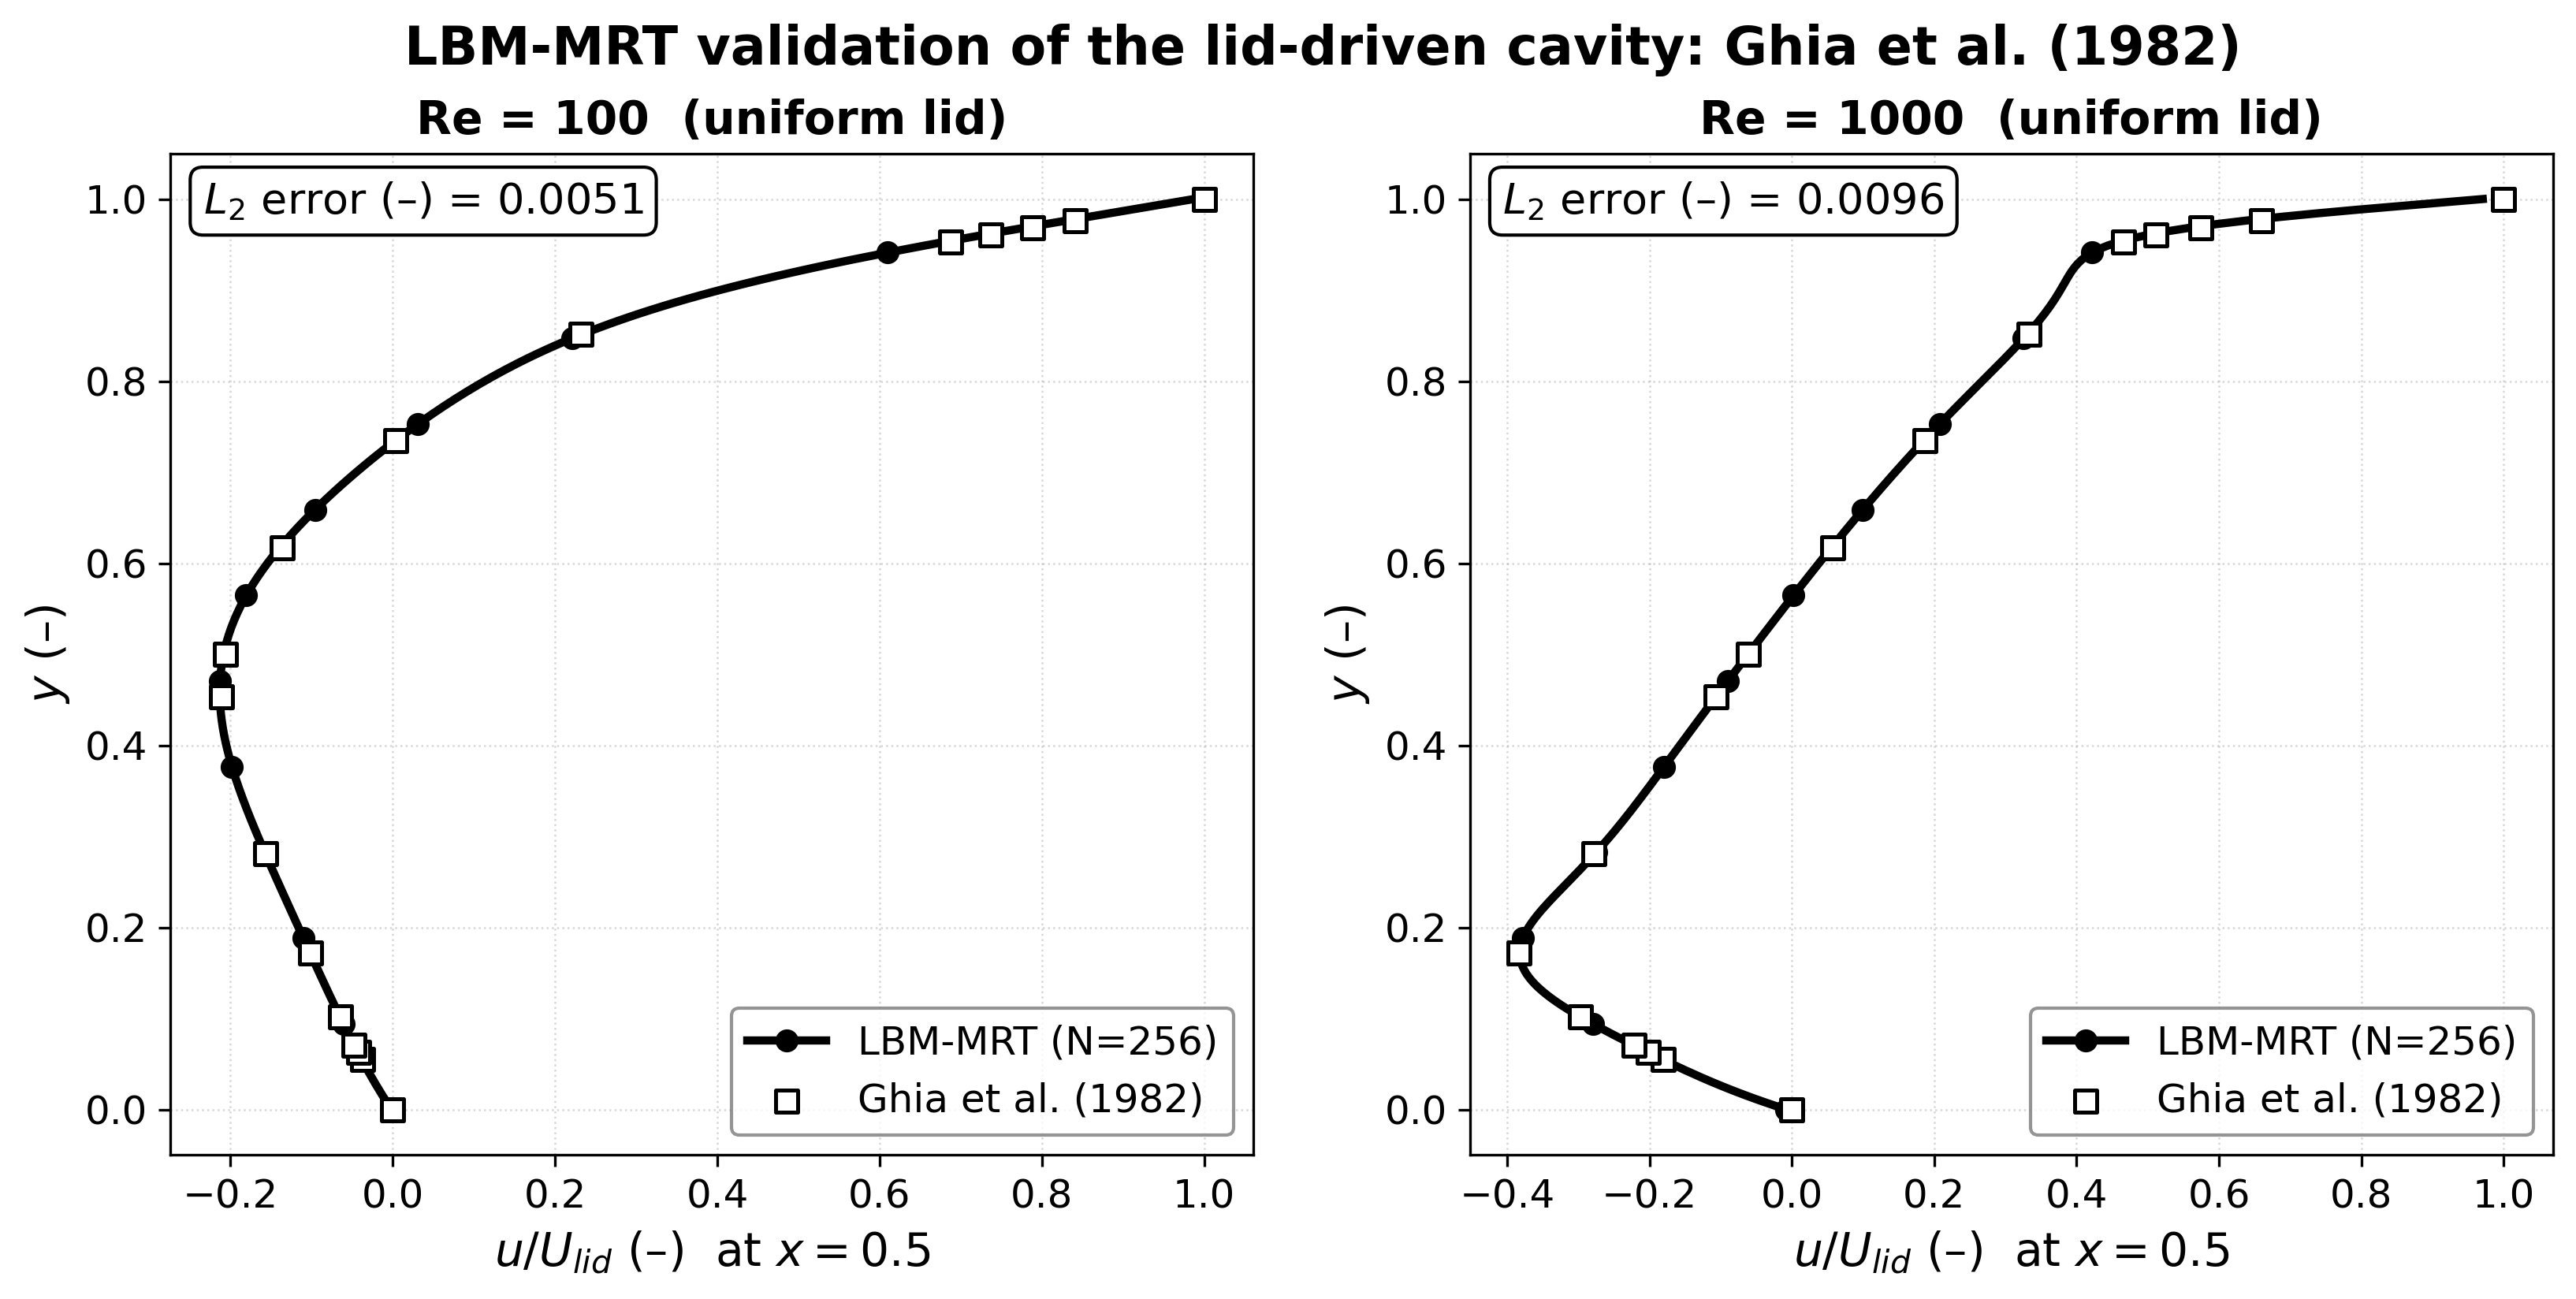
\includegraphics[width=\textwidth]{figS9_ghia_validation.png}
\caption{Square-cavity LBM center-line velocity profiles versus Ghia et al.\
(1982), $Re=100$ (left) and $Re=1000$ (right), uniform lid, $N=256$.
The in-panel $L_2$ values correspond to the center-line errors reported in
\color{blue}
Table~\ref{tab:ghia}.}
\alttext{Square-cavity LBM center-line velocity profiles versus Ghia et al.\ (1982), $Re=100$ (left) and $Re=1000$ (right), uniform lid, $N=256$. The in-panel $L_2$ values correspond to the center-line errors reported in Table~.}



\label{fig:ghia}
\color{black}
\end{figure}


\subsection{Curved-boundary test (exact rigid rotation)}
The curved-boundary implementation is verified against the exact stationary
solution $u=(y,-x)$ of a fully rotating disk, which is independent of $Re$.
\color{blue}
At fixed lid velocity the $L_2$ error of this test stagnates near $10^{-3}$ as
the grid is refined, because the residual error is set by the lattice Mach
number of the fixed $U_{\mathrm{lid}}$. Table~\ref{tab:rotation} reports the same
test in a diffusive scaling, $U_{\mathrm{lid}}(N)=0.05\times32/N$, which keeps
$Re=100$ and $\tau\simeq0.547$ fixed while the lattice Mach number decreases as
$1/N$. The error then decreases monotonically, with observed orders $1.88$,
$1.90$ and $1.93$ between successive grids. The companion
fixed-$U_{\mathrm{lid}}$ runs corroborate the lattice-Mach interpretation
through the wall-normal leakage $\max|u\cdot m|$, which decreases from
$4.41\times10^{-5}$ at $N=32$ to $2.06\times10^{-5}$ at $N=96$. Because the
production campaign holds $U_{\mathrm{lid}}=0.05$ at every resolution, the same
lattice-Mach offset (of order $10^{-3}$ in this $L_2$) is present in all of its
fields; being constant in $N$, it cannot explain the $18.1$--$25.4\,\%$ drift
of $D/A$ between $N=128$ and $N=256$.
\color{black}
% ------------------------------------------------------------------
\color{blue}
\begin{table}[H]
\color{black}
\centering
\caption{Curved-boundary verification on the exact rigid-rotation solution
\color{blue}
$u=(y,-x)$ of a rotating disk at $Re=100$, in diffusive scaling
$U_{\mathrm{lid}}(N)=0.05\times32/N$: $L_2$/$L_\infty$ errors, lid velocity,
iterations and final residual.}
\alttext{Curved-boundary verification on the exact rigid-rotation solution $u=(y,-x)$ of a rotating disk at $Re=100$, in diffusive scaling $U_{lid}(N)=0.05\times32/N$: $L_2$/$L_\infty$ errors, lid velocity, iterations and final residual.}



\label{tab:rotation}
\begin{tabular}{@{}lccccc@{}}
\toprule
$N$ & $U_{\mathrm{lid}}$ & $L_2$ & $L_\infty$ & Iterations & Residual \\
\midrule
32 & 0.0500 & $9.35\times10^{-4}$ & $1.29\times10^{-3}$ & 18\,500 & $9.57\times10^{-11}$ \\
48 & 0.0333 & $4.36\times10^{-4}$ & $5.95\times10^{-4}$ & 38\,900 & $9.96\times10^{-11}$ \\
64 & 0.0250 & $2.52\times10^{-4}$ & $3.42\times10^{-4}$ & 65\,800 & $9.78\times10^{-11}$ \\
96 & 0.0167 & $1.15\times10^{-4}$ & $1.55\times10^{-4}$ & 136\,700 & $9.97\times10^{-11}$ \\
\bottomrule
\end{tabular}
\color{black}
\end{table}

\subsection{LBM--FEM cross-validation over the superelliptic family}
\color{blue}
\label{sec:solverc}
\color{black}

\color{blue}
To validate the MRT-LBM solver across the geometric family, an independent cross-validation is performed against a Taylor--Hood quadratic-velocity/linear-pressure (P2/P1) finite-element solver. Table~\ref{tab:lbmfem} reports interior relative $L_2$ discrepancies at the available $(N,Re)$ comparison levels, including the reference resolution $N=128$ at $Re=400$ for the sharpest ($n=1.25$, $1.39\,$%) and near-square ($n=4$, $0.78\,$%) members. At fixed finite-element mesh, halving the lattice spacing reduces the $n=4$ discrepancy from $1.45\,$% to $0.78\,$%, locating the dominant remaining difference on the lattice side. The pointed tip remains the worst case, consistent with the tighter radius of curvature resolved by the interpolated bounce-back scheme. The additional $N=256$ comparison decreases the discrepancy to $0.60\,$% and $0.25\,$%, but refines both discretisations and therefore does not attribute the residual to either side.
\color{black}

\color{blue}
The resolution study in Fig.~\ref{fig:lbmfemconv} shows that the interior LBM--FEM discrepancy decreases from $1.48\times10^{-2}$ at $N=32$ to $2.20\times10^{-3}$ at $N=96$ on the circle at $Re=100$. This decrease is reported as a sensitivity check over the tested grids; it is not used to claim a converged asymptotic error or to transfer a formal convergence rate to the production cases.
\color{black}


% ------------------------------------------------------------------
\color{blue}
\begin{table}[H]
\color{black}
\centering
\caption{Interior relative $L_2$ discrepancy (\%) between MRT-LBM and the
\color{blue}
independent Taylor--Hood $\mathbb{P}_2/\mathbb{P}_1$ FEM solution, tabulated by
comparison level. The lattice resolution $N$ and the finite-element refinement
$n_{\mathrm{refs}}$ are independent discretisation levels and are not matched
to one another; each row therefore states the mesh it actually used, as
triangle and total-unknown counts ($2(V+E)+V$) measured on the assembled
mesh, so that the finite-element side of every comparison is fully specified.
$N=64$ at $Re=100$ and $N=96$ at $Re=400$ are the original cross-checks;
$N=128$ at $Re=400$ brings the comparison to the reference resolution of the
database and $n=1.25$ to the family, and it is made against the same
$74\,371$-unknown mesh as the $N=96$ row; $N=256$ at $Re=400$ is an additional refined comparison, and because it refines the
lattice and the finite-element mesh together ($65\,536$ triangles, $296\,195$
unknowns) it cannot attribute the residual to either side --- it only checks
that the discrepancy decreases and that the pointed tip stays the worst of the
family. At that level the discrepancy is evaluated on the intersection of the
two discretisations: $24$ of the $60\,132$ LBM fluid nodes of the $n=4$ case
fall outside the assembled triangulation and are excluded from both metrics,
against $0$ for $n=1.25$. All LBM residuals below $10^{-8}$;
every FEM solve converged, in $22$ Picard iterations at
$n_{\mathrm{refs}}=6$ and in $18$ and $22$ at $n_{\mathrm{refs}}=7$.}
\alttext{Interior relative $L_2$ discrepancy (\%) between MRT-LBM and the independent Taylor--Hood $\mathbb{P}_2/\mathbb{P}_1$ FEM solution, tabulated by comparison level. The lattice resolution $N$ and the finite-element refinement $n_{refs}$ are independent discretisation levels and are not matched to one another; each row therefore states the mesh it actually used, as triangle and total-unknown counts ($2(V+E)+V$) measured on the assembled mesh, so that the finite-element side of every comparison is fully specified. $N=64$ at $Re=100$ and $N=96$ at $Re=400$ are the original cross-checks; $N=128$ at $Re=400$ brings the comparison to the reference resolution of the database and $n=1.25$ to the family, and it is made against the same $74\,371$-unknown mesh as the $N=96$ row; $N=256$ at $Re=400$ is an additional refined comparison, and because it refines the lattice and the finite-element mesh together ($65\,536$ triangles, $296\,195$ unknowns) it cannot attribute the residual to either side --- it only checks that the discrepancy decreases and that the pointed tip stays the worst of the family. At that level the discrepancy is evaluated on the intersection of the two discretisations: $24$ of the $60\,132$ LBM fluid nodes of the $n=4$ case fall outside the assembled triangulation and are excluded from both metrics, against $0$ for $n=1.25$. All LBM residuals below $10^{-8}$; every FEM solve converged, in $22$ Picard iterations at $n_{refs}=6$ and in $18$ and $22$ at $n_{refs}=7$.}



\label{tab:lbmfem}
\tabbox{%
\begin{tabular}{@{}lccccc@{}}
\toprule
comparison level & $n=1.25$ & $n=1.5$ & $n=2$ & $n=4$ & square \\
\midrule
$Re=100$, $N=64$, $n_{\mathrm{refs}}=5$, $4\,096$ triangles, $18\,755$ unknowns & -- & 1.06 & 0.93 & 0.96 & 0.87 \\
$Re=400$, $N=96$, $n_{\mathrm{refs}}=6$, $16\,384$ triangles, $74\,371$ unknowns & -- & 1.20 & 1.20 & 1.45 & 1.21 \\
$Re=400$, $N=128$, $n_{\mathrm{refs}}=6$, $16\,384$ triangles, $74\,371$ unknowns & 1.39 & -- & -- & 0.78 & -- \\
$Re=400$, $N=256$, $n_{\mathrm{refs}}=7$, $65\,536$ triangles, $296\,195$ unknowns & 0.60 & -- & -- & 0.25 & -- \\
\bottomrule
\end{tabular}%
}
\color{black}
\end{table}

\color{blue}
\begin{figure}[H]
\color{black}
\centering
\begin{subfigure}[b]{0.48\textwidth}
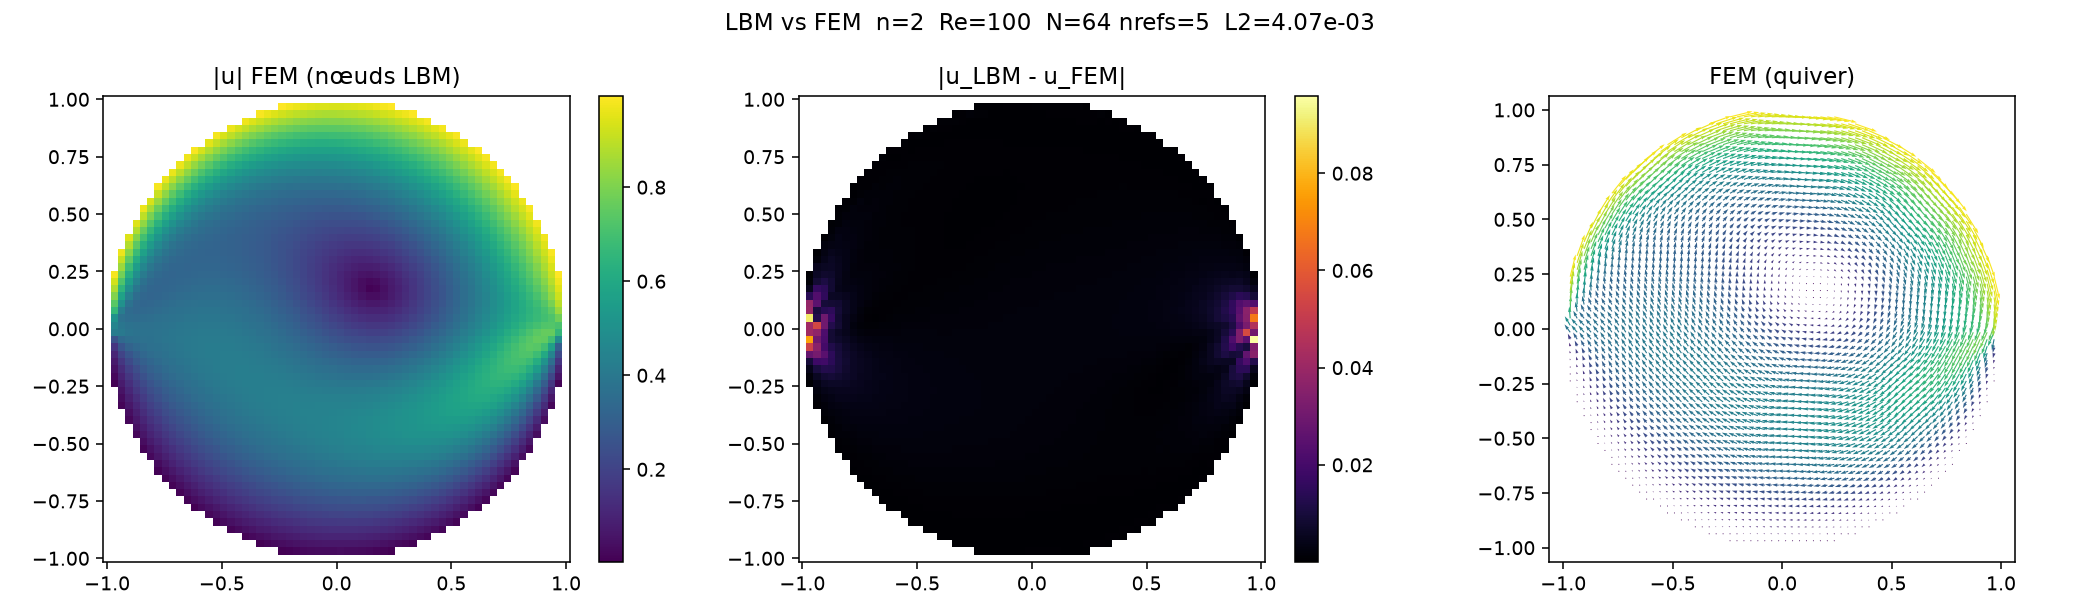
\includegraphics[width=\textwidth]{lbm_fem_circle_Re100_N64.png}
\caption{Circle ($n=2$), $Re=100$}
\end{subfigure}
\hfill
\begin{subfigure}[b]{0.48\textwidth}
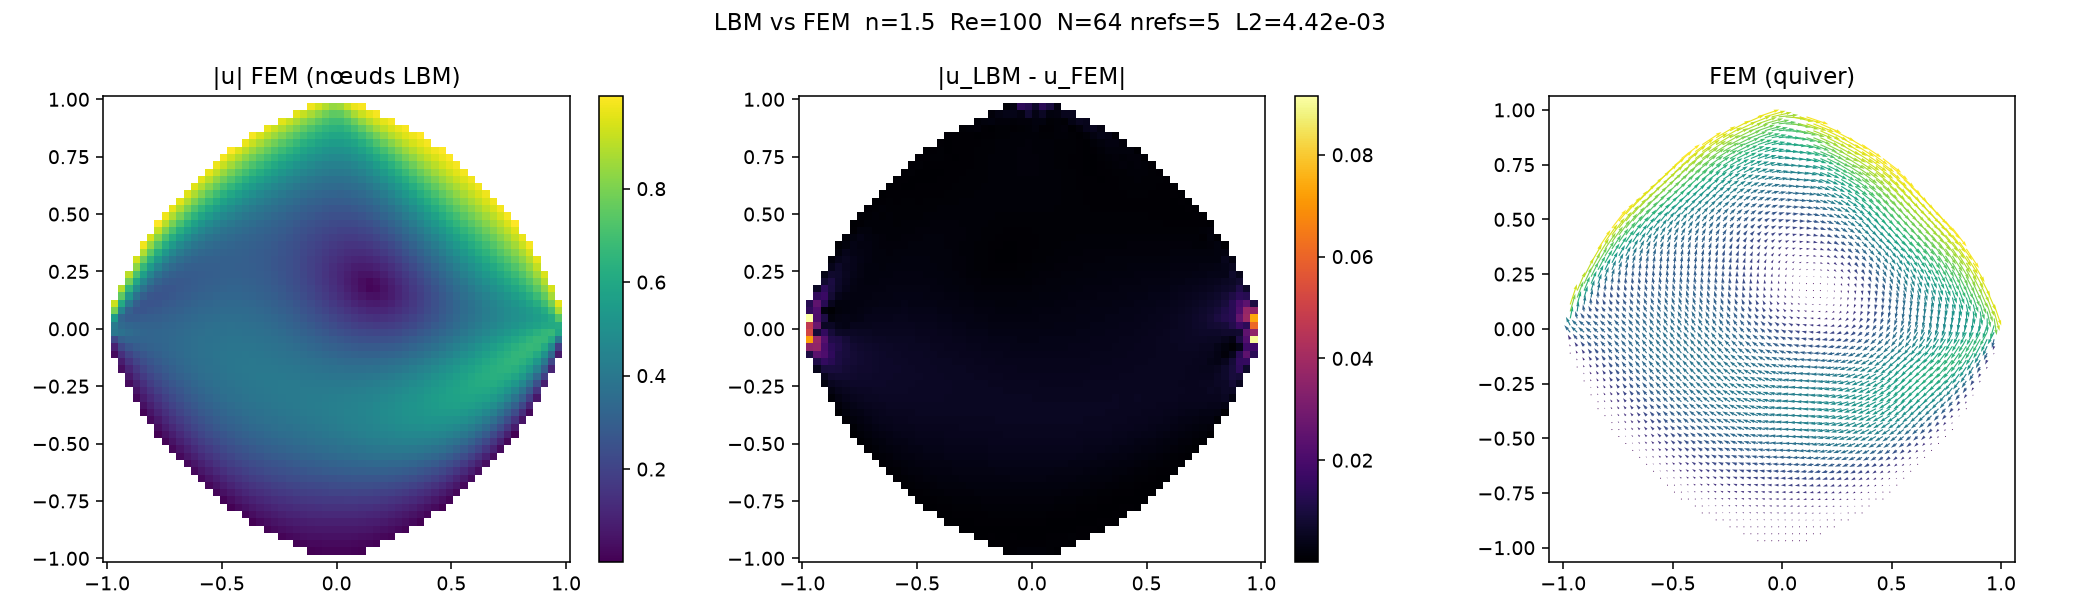
\includegraphics[width=\textwidth]{lbm_fem_ell1.5_Re100_N64.png}
\caption{Ellipse ($n=1.5$), $Re=100$}
\end{subfigure}
\vspace{0.3cm}
\begin{subfigure}[b]{0.48\textwidth}
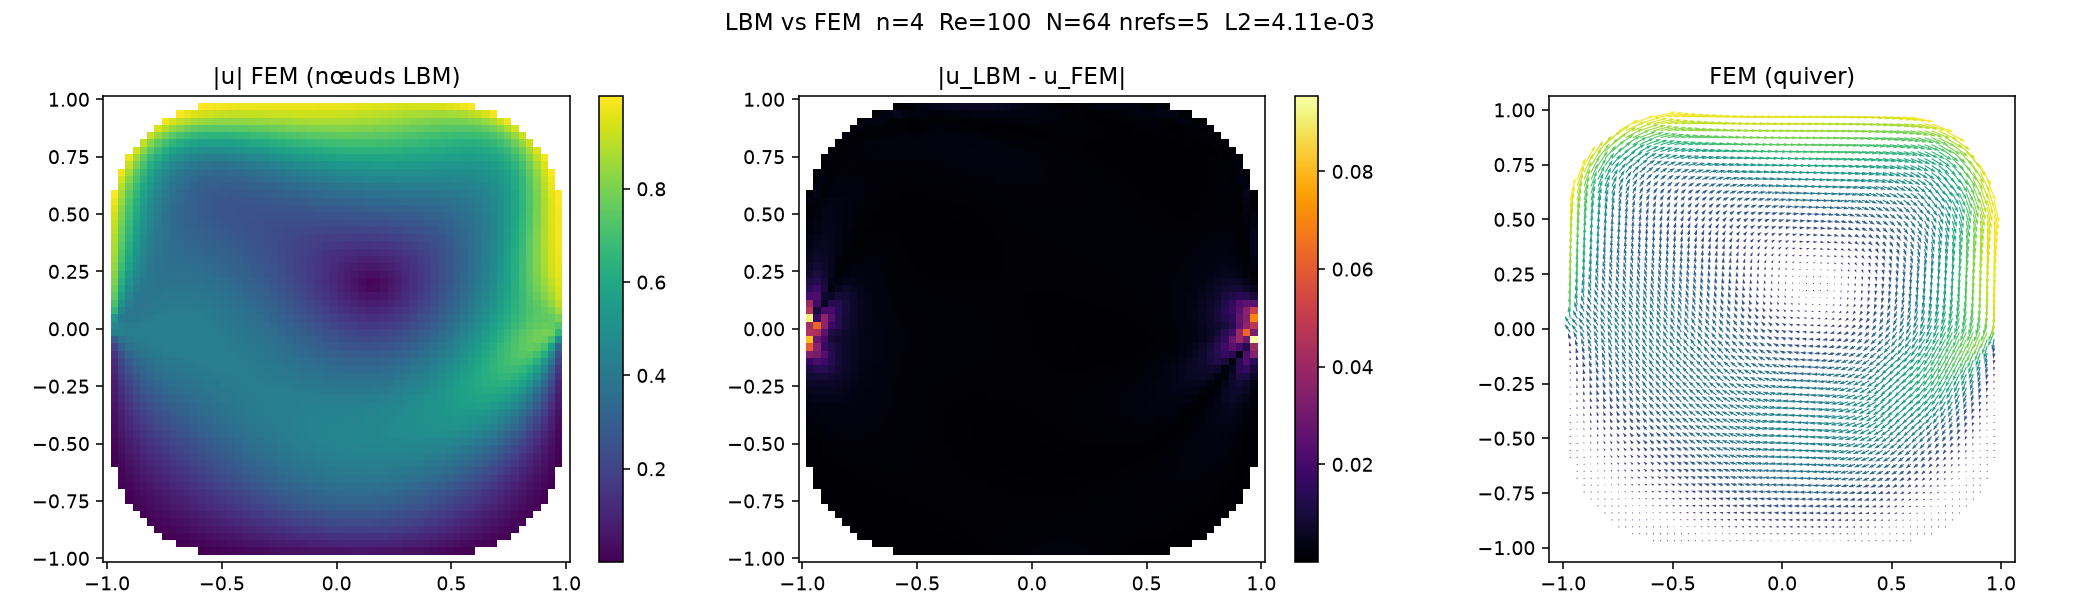
\includegraphics[width=\textwidth]{lbm_fem_ell4_Re100_N64.png}
\caption{Super-ellipse ($n=4$), $Re=100$}
\end{subfigure}
\hfill
\begin{subfigure}[b]{0.48\textwidth}
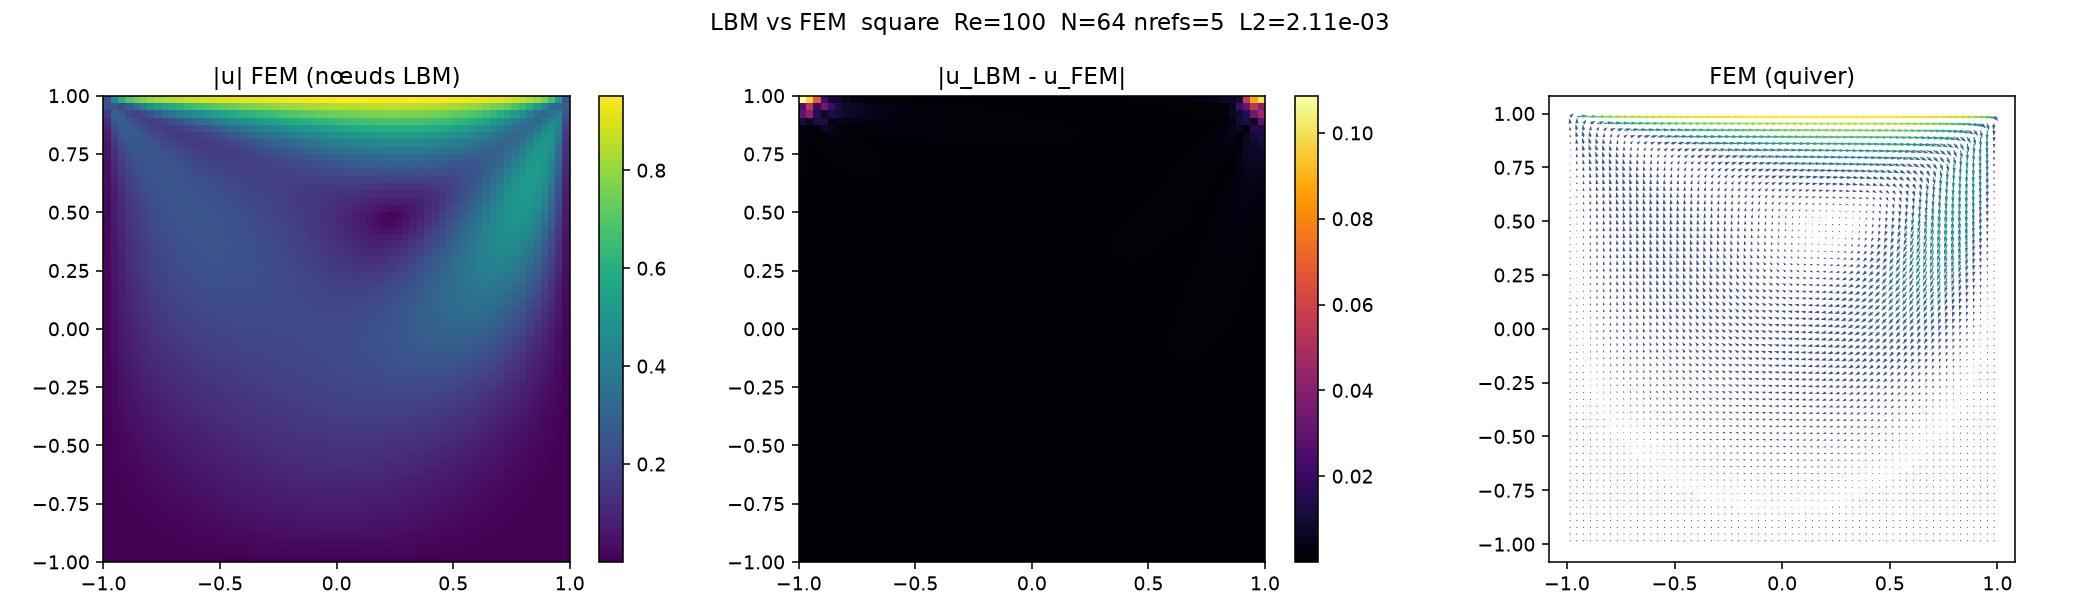
\includegraphics[width=\textwidth]{lbm_fem_square_Re100_N64.png}
\caption{Square, $Re=100$}
\end{subfigure}
\caption{LBM--FEM velocity-field comparison at $Re=100$ for four cavity geometries
\color{blue}
(lattice $N=64$, finite-element mesh $n_{\mathrm{refs}}=5$, $4\,096$ triangles). Each panel overlays the LBM and FEM
\color{black}
streamlines on the LBM velocity magnitude. The corresponding interior relative
\color{blue}
$L_2$ discrepancies are reported in Table~\ref{tab:lbmfem}.}
\alttext{LBM--FEM velocity-field comparison at $Re=100$ for four cavity geometries (lattice $N=64$, finite-element mesh $n_{refs}=5$, $4\,096$ triangles). Each panel overlays the LBM and FEM streamlines on the LBM velocity magnitude. The corresponding interior relative $L_2$ discrepancies are reported in Table~.}



\label{fig:lbmfem100}
\color{black}
\end{figure}

\color{blue}
\begin{figure}[H]
\color{black}
\centering
\begin{subfigure}[b]{0.48\textwidth}
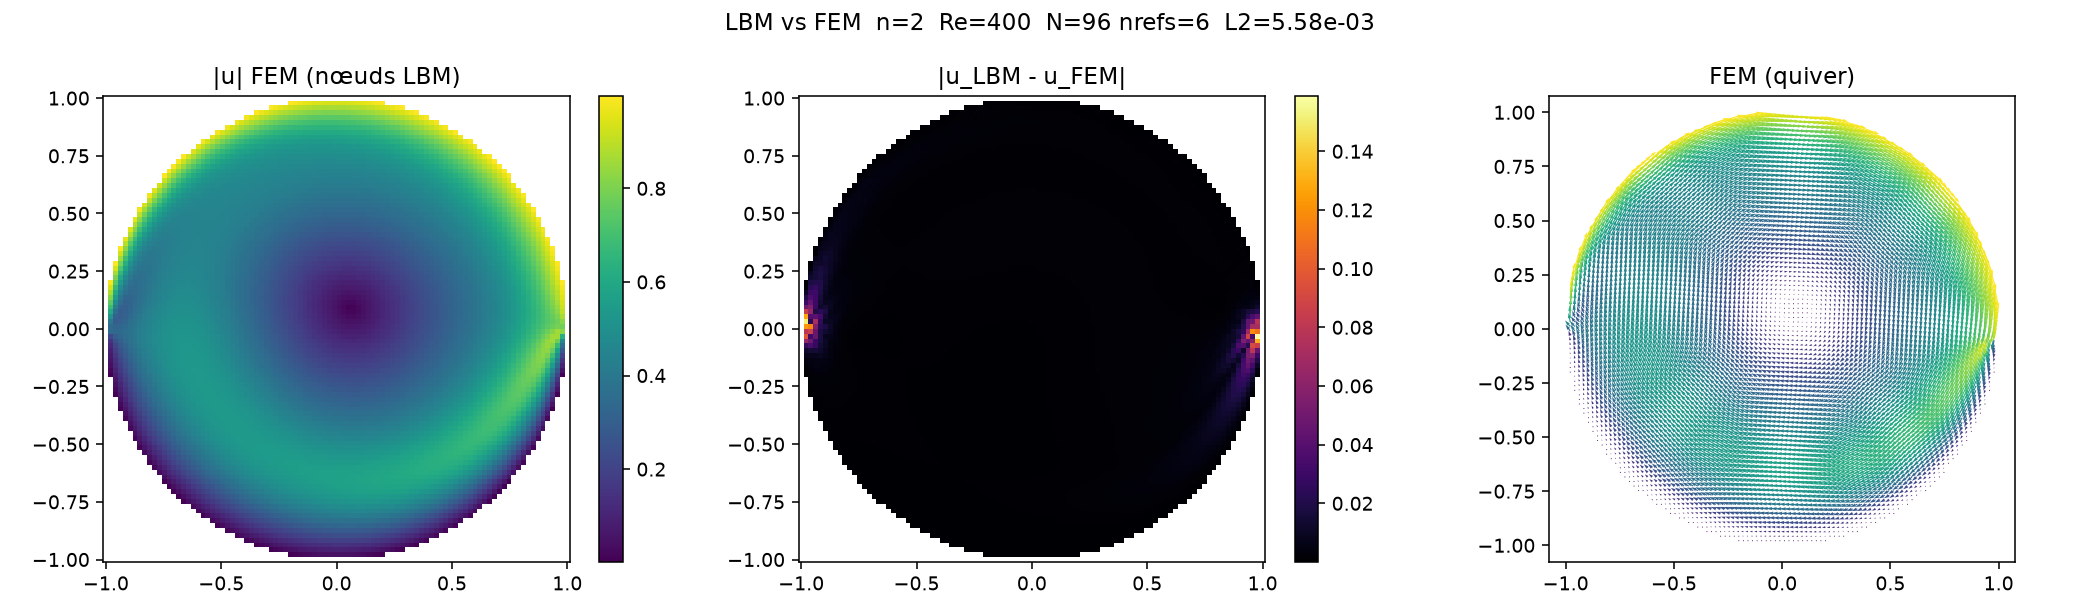
\includegraphics[width=\textwidth]{lbm_fem_circle_Re400_N96.png}
\caption{Circle ($n=2$), $Re=400$}
\end{subfigure}
\hfill
\begin{subfigure}[b]{0.48\textwidth}
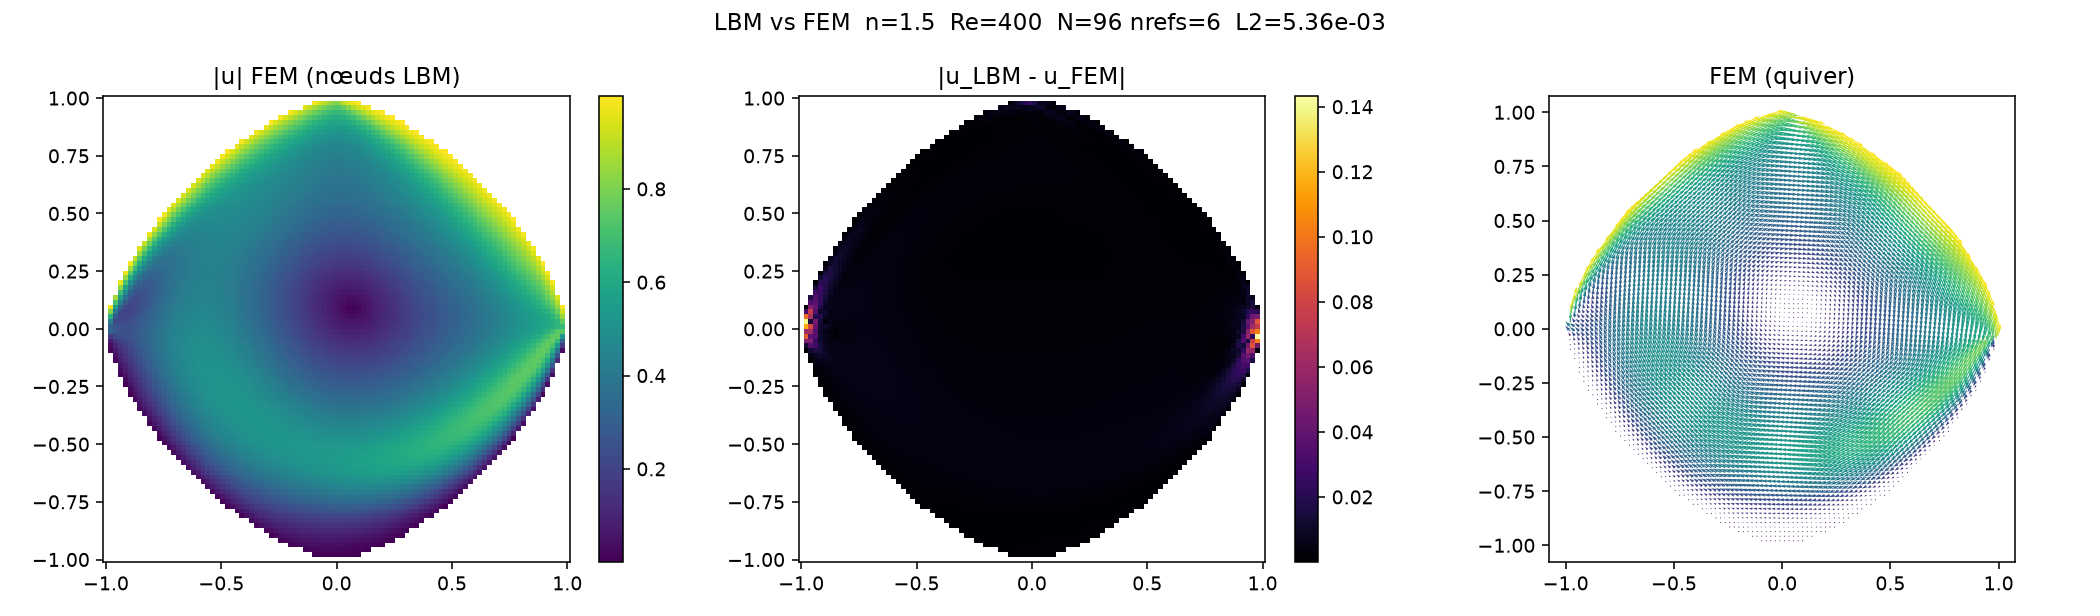
\includegraphics[width=\textwidth]{lbm_fem_ell1.5_Re400_N96.png}
\caption{Ellipse ($n=1.5$), $Re=400$}
\end{subfigure}
\vspace{0.3cm}
\begin{subfigure}[b]{0.48\textwidth}
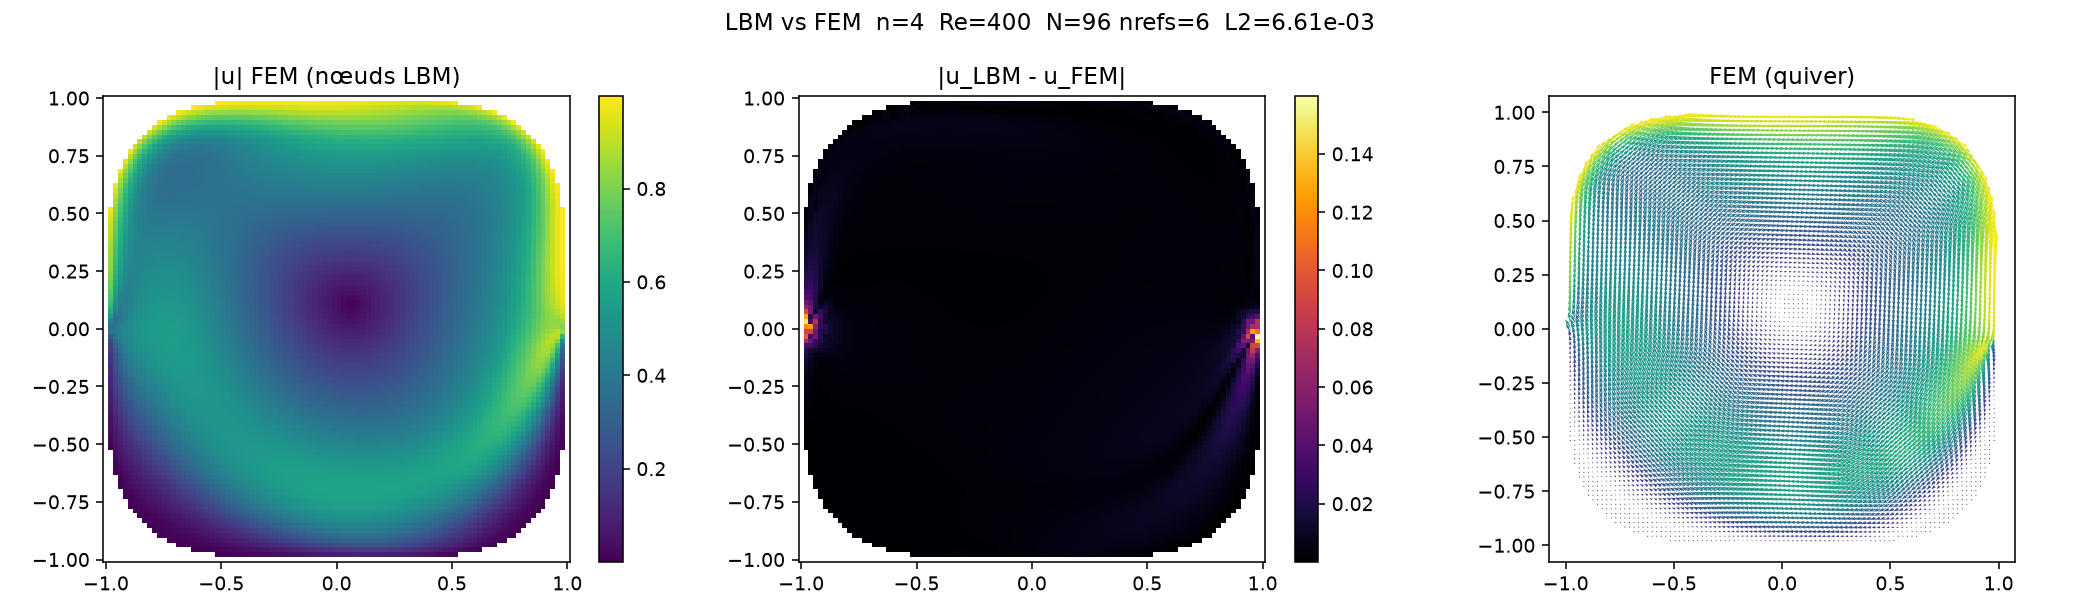
\includegraphics[width=\textwidth]{lbm_fem_ell4_Re400_N96.png}
\caption{Super-ellipse ($n=4$), $Re=400$}
\end{subfigure}
\hfill
\begin{subfigure}[b]{0.48\textwidth}
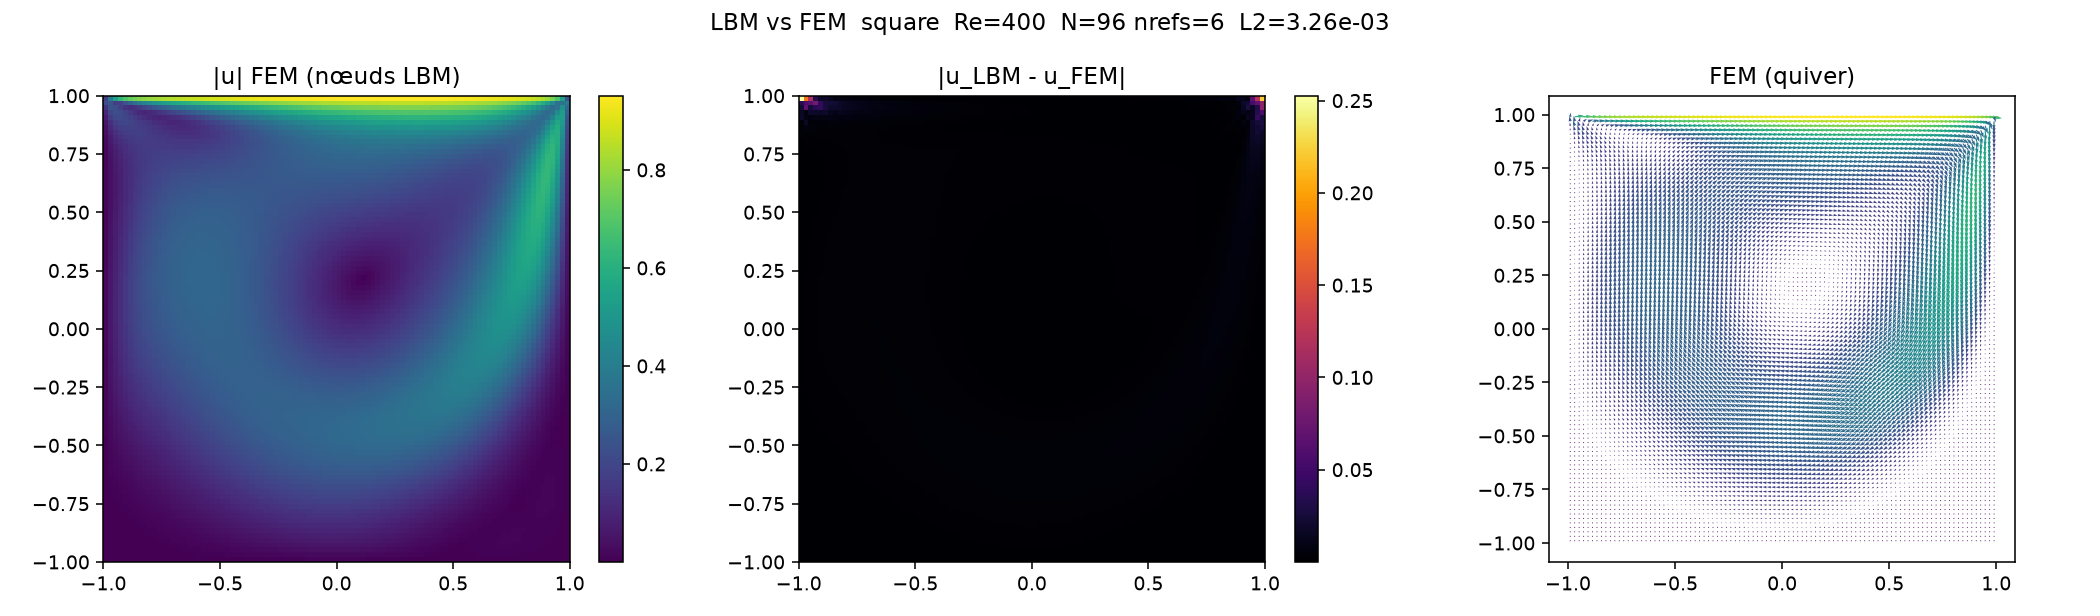
\includegraphics[width=\textwidth]{lbm_fem_square_Re400_N96.png}
\caption{Square, $Re=400$}
\end{subfigure}
\caption{LBM--FEM velocity-field comparison at $Re=400$ for four cavity geometries
\color{blue}
(lattice $N=96$, finite-element mesh $n_{\mathrm{refs}}=6$, $16\,384$ triangles). The comparison remains within the reported
\color{black}
discretization-error range, with all interior relative $L_2$ discrepancies
\color{blue}
below $1.5\,\%$ (Table~\ref{tab:lbmfem}).}
\alttext{LBM--FEM velocity-field comparison at $Re=400$ for four cavity geometries (lattice $N=96$, finite-element mesh $n_{refs}=6$, $16\,384$ triangles). The comparison remains within the reported discretization-error range, with all interior relative $L_2$ discrepancies below $1.5\,\%$ (Table~).}



\label{fig:lbmfem400}
\color{black}
\end{figure}

\color{blue}
\begin{figure}[H]
\color{black}
\centering
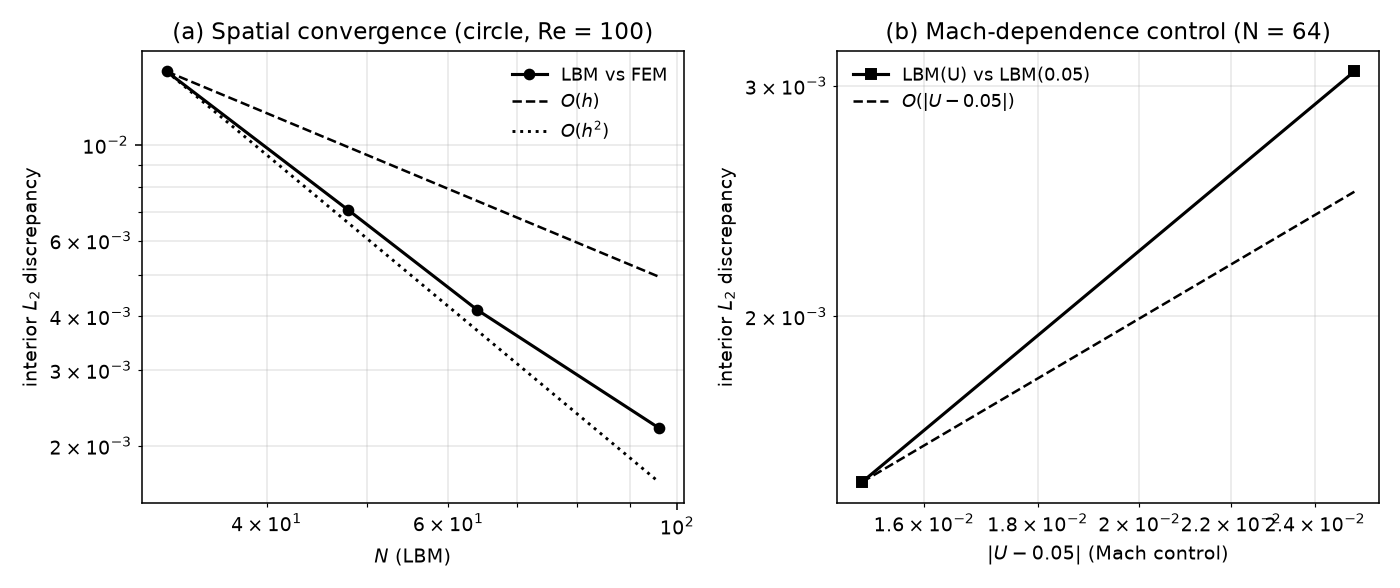
\includegraphics[width=0.70\textwidth]{figS11b_lbm_fem_convergence_N.png}
\caption{Grid dependence of the LBM--FEM interior relative $L_2$ discrepancy
for the circular cavity at $Re=100$ as the LBM resolution is refined from
$N=32$ to $N=96$. The observed decrease is consistent with a reduction of
discretization error over the tested resolutions.}
\color{blue}
\alttext{Grid dependence of the LBM--FEM interior relative $L_2$ discrepancy for the circular cavity at $Re=100$ as the LBM resolution is refined from $N=32$ to $N=96$. The observed decrease is consistent with a reduction of discretization error over the tested resolutions.}



\label{fig:lbmfemconv}
\color{black}
\end{figure}

% ======================================================================
\color{blue}

\section{Database quality control}\label{sec:database}
\color{black}
Every one of the $126$ processed configurations passed the fixed
quality-control protocol before being accepted into the database; this section details the report for
\color{blue}
the $190$-case physics-analysis subset (all $10$ exponents $n$ at the $19$
Reynolds numbers of the complete grid, $N=128$). Table~\ref{tab:qc} condenses the
quality-control report: $190$ cases found
\color{black}
and analysed, zero failures, maximum relative area error of the discretized
\color{blue}
domain $0.948\,\%$ (below the $1\,\%$ acceptance threshold), maximum LBM residual
$9.9999\times10^{-9}$ (below $1\times10^{-8}$), and positive minimum density.
\color{black}
Because the tangential moving-lid boundary condition
\color{blue}
$u_w=U_{\mathrm{lid}}(m_y,-m_x)$ is not invariant under reflection
\color{black}
$x\mapsto-x$, mirror symmetry is not a valid numerical quality criterion for
this database and is explicitly excluded from the quality control
\color{blue}
(\emph{not applicable} status). Fig.~\ref{fig:areaerror} shows the spatial
\color{black}
distribution of the area error over the $n\times Re$ grid.

The database maximum of the finite-difference divergence, $|\nabla\cdot u|=1.67$
\color{blue}
(Table~\ref{tab:qc}), is attained at a single isolated interior cell of the most
\color{black}
pointed configuration ($n=1.25$, $Re=1000$), at $x\approx-0.953$,
$y\approx0.024$, i.e.\ about three cell widths from the wall in the sharp
curved-tip region; its four-point stencil is entirely fluid, so the value is
not a boundary-stencil artifact, but it is consistent with the strong local
curvature-approximation error of the curved moving boundary at the sharp
vertex. It is reported as a local, geometry-specific finite-resolution
excursion rather than a systematic feature of the database.
\color{blue}

Recomputing the same diagnostic on the $50$-case $N=256$ campaign confirms
this reading. The per-case maximum scales with the stencil length, as expected
for a finite-difference derivative of a discrete field: its median over the
database rises from $1.31$ at $N=128$ ($190$ cases) to $2.43$ at $N=256$
($50$ cases). The individual outlier grows on that same trend, from $1.67$ to
$2.72$ --- a factor $1.63$, against $1.85$ for the median --- which is what a
tip-localised structure whose discrete gradient steepens with $h$ does, and not
what a spurious error does: refining resolves it further instead of removing
it. The case $(n,Re)=(1.25,1000)$ still carries the largest value,
$\max|\nabla\cdot u|=2.72$, but now by only $12\,\%$ above the $N=256$ median
(against $27\,\%$ at $N=128$), and the maximum migrates to the opposite tip
($x\approx0.977$, $y\approx0.012$) with the left--right asymmetry of the
tangential drive. The excursion is therefore a resolution-scaling
finite-difference signature of the sharp tip, not a physical divergence of
the field. Its weight in the reported observables is negligible: removing the
single worst cell changes $D/A$ by $-0.06\,\%$ at $N=128$ and $-0.07\,\%$ at
$N=256$, and removing the $20$ worst cells by $-4.2\,\%$ and $-2.6\,\%$
respectively.
\color{black}
% ------------------------------------------------------------------
\color{blue}
\begin{table}[H]
\color{black}
\centering
\color{blue}
\caption{Database quality-control summary ($190$ cases analysed, $N=128$).}
\alttext{Database quality-control summary ($190$ cases analysed, $N=128$).}



\label{tab:qc}
\begin{tabular}{@{}lll@{}}
\toprule
Metric & Value & Status \\
\midrule
Cases found / analysed & 190 / 190 & --- \\
Failed cases & 0 & --- \\
Max.\ relative area error & $9.479\times10^{-3}$ & pass ($<10^{-2}$) \\
Max.\ LBM residual & $9.9999\times10^{-9}$ & pass ($<10^{-8}$) \\
Min.\ density $\rho_{\min}$ & $0.9954$ & pass ($>0$) \\
Max.\ $|\nabla\cdot u|$ & $1.67$ & reported (no gate) \\
Mirror symmetry & not applicable & excluded (tangent-lid boundary condition) \\
\bottomrule
\end{tabular}
\color{black}
\end{table}

\color{blue}
\begin{figure}[H]
\color{black}
\centering
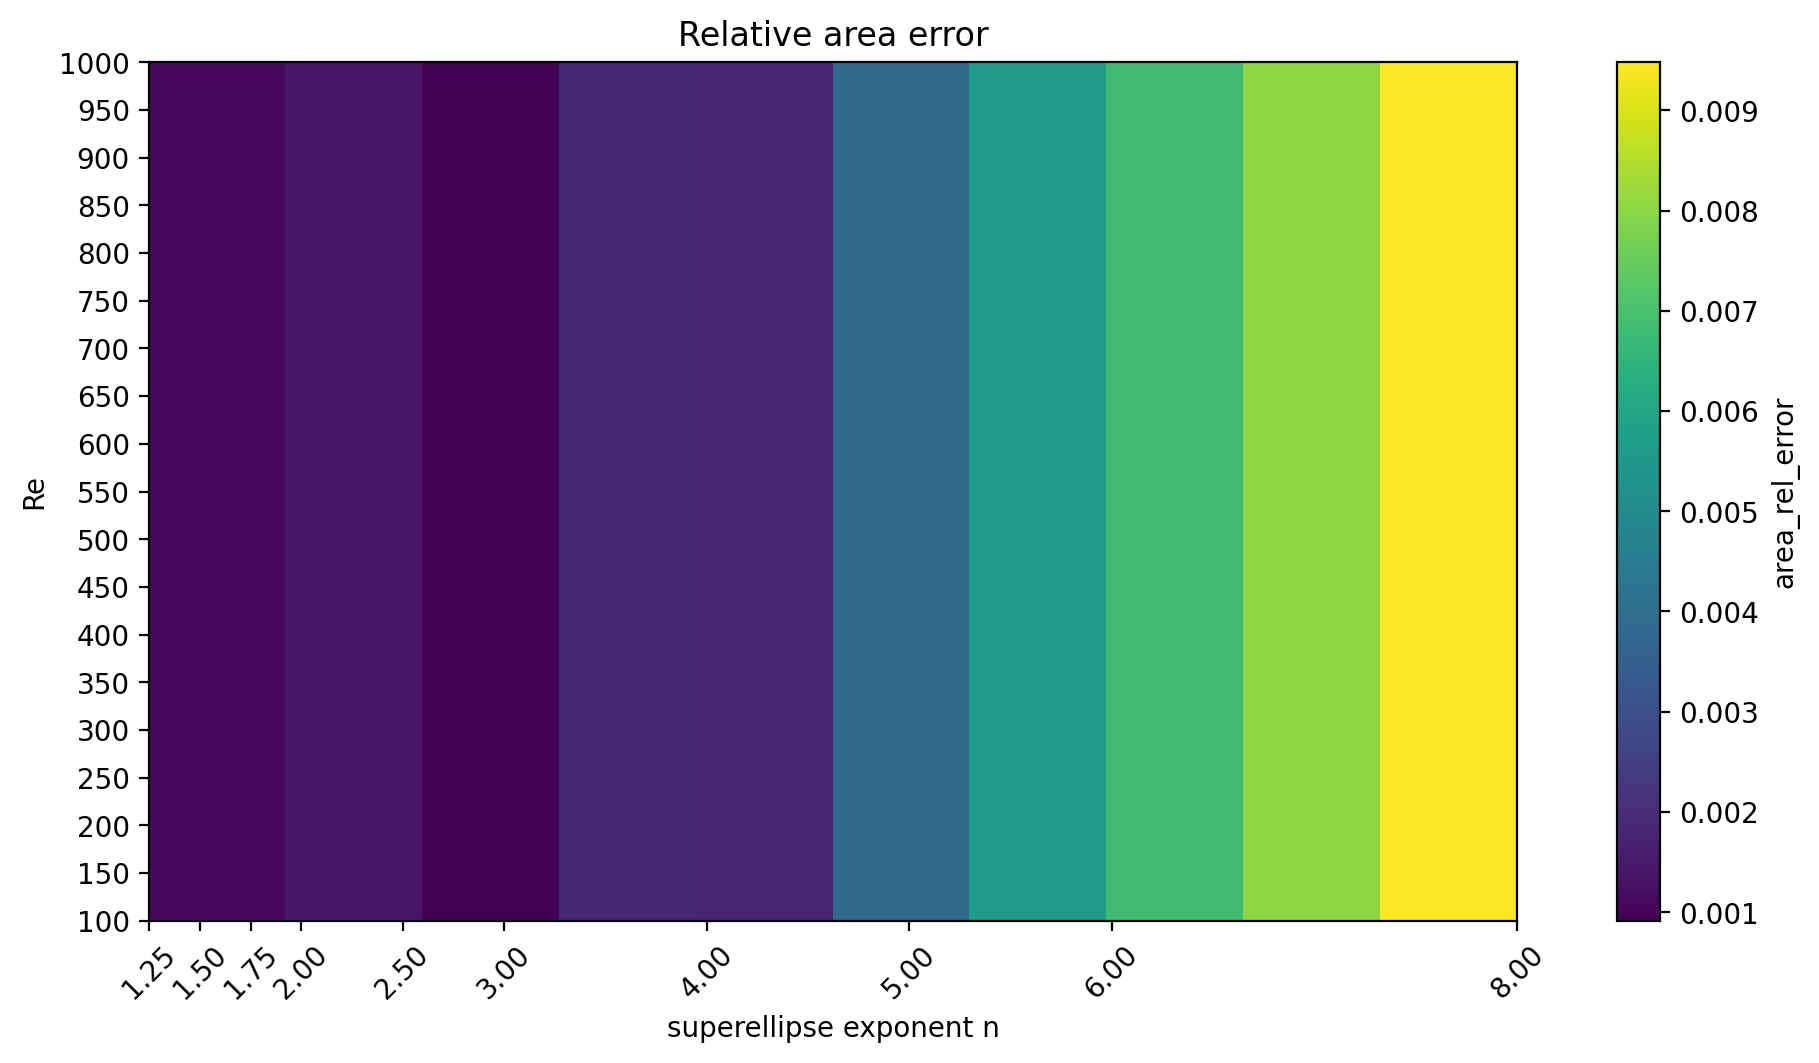
\includegraphics[width=\textwidth]{map_area_error.png}
\caption{Relative area error of the discretized domain over the
$n\times Re$ grid of the analysed subset. All
values are below the $1\,\%$ threshold.}
\color{blue}
\alttext{Relative area error of the discretized domain over the $n\times Re$ grid of the analysed subset. All values are below the $1\,\%$ threshold.}



\label{fig:areaerror}
\color{black}
\end{figure}

\color{blue}

\section{Physical observables of the comparison configurations}\label{sec:observables}
\color{black}
All physical observables reported in this section are computed from the
$N=128$ LBM reference fields.
The velocity derivatives are evaluated by second-order central differences on
the interior nodes whose four-point stencil is entirely fluid; the vorticity
is $\omega=\partial v/\partial x-\partial u/\partial y$; the streamfunction is
a diagnostic reconstruction obtained from the Poisson problem
$\nabla^2\psi=-\omega$ with $\psi=0$ on the discrete fluid boundary
(convention $u=\psi_y$, $v=-\psi_x$); the kinetic energy is
$KE=\int_{\Omega}\tfrac{1}{2}|\mathbf{u}|^2\,dA$ over the fluid mask; the
viscous dissipation is the standard mechanical dissipation of the
incompressible Newtonian fluid, $D=2\nu\int_{\Omega}S:S\,dA$, which evaluates
with $\nu=2/Re$ as
$D=\tfrac{4}{Re}\int_{\Omega}\left[(\partial u/\partial x)^2
+(\partial v/\partial y)^2+\tfrac{1}{2}(\partial u/\partial y+\partial
v/\partial x)^2\right]dA$ over the valid-gradient mask; and the enstrophy is
$\mathcal{E}=\tfrac{1}{2}\int_{\Omega}\omega^2\,dA$. The maximum velocity is
$U_{\max}=\max_{\Omega}|\mathbf{u}|$. Vortex counts are obtained from the
connected extrema of $\psi$ on the fluid core (nodes at Euclidean distance
$\geq 2$ from the wall), with threshold
$\tau=\max\left(\tfrac{q}{100}\,|\psi_{\mathrm{primary}}|,\,10^{-14}\right)$
\color{blue}
for $q\in\{1,3,5\}\,\%$. The area-normalized kinetic energy of Table~\ref{tab:energy30} is obtained by
dividing $KE$ by the exact cavity area $A(n)=4\,\Gamma(1+1/n)^2/\Gamma(1+2/n)$
for $a=b=1$ (the area formula in the main manuscript), whereas $D/A$ is
divided by the area $A_{\rm mask}(n)$ of the discrete integration mask that
carries the sum defining $D$, so that numerator and denominator share the same
support.
\color{black}

\color{blue}
Table~\ref{tab:observables} provides numerical values of the physical observables
for four representative configurations spanning the geometry family. These
values facilitate quantitative inspection of the reference fields and document
the flow characteristics independently of any surrogate model. The table includes maximum velocity,
\color{black}
maximum absolute vorticity, primary streamfunction, vortex counts at the
$1\,\%$ and $5\,\%$ thresholds, dissipation, kinetic energy, enstrophy and the
root-mean-square divergence of the reference fields. The physical trends over
the complete $n$--$Re$ parameter space are discussed in the physical-analysis
sections of the main manuscript.
% ------------------------------------------------------------------
\color{blue}
\begin{table}[H]
\color{black}
\centering
\caption{Physical observables of the four comparison configurations
($N=128$): maximum speed, maximum
absolute vorticity, primary streamfunction, vortex count at the $1\,\%$ /
$5\,\%$ thresholds, dissipation, kinetic energy, enstrophy and
root-mean-square (RMS) divergence.}
\color{blue}
\alttext{Physical observables of the four comparison configurations ($N=128$): maximum speed, maximum absolute vorticity, primary streamfunction, vortex count at the $1\,\%$ / $5\,\%$ thresholds, dissipation, kinetic energy, enstrophy and root-mean-square (RMS) divergence.}



\label{tab:observables}
\tabbox{%
\begin{tabular}{@{}lcccccccc@{}}
\toprule
Case & $U_{\max}$ & $|\omega|_{\max}$ & $\psi_{\mathrm{prim}}$ &
$n_{\mathrm{vort}}^{1\%}/n_{\mathrm{vort}}^{5\%}$ & Dissipation & KE &
Enstrophy & RMS$\;|\nabla\cdot u|$ \\
\midrule
$n=2,Re=400$           & 0.998 & 21.4  & $-0.337$ & 1 / 1 & 0.0467 & 0.357 & 7.69 & 0.0334 \\
$n=3,Re=1000$          & 1.039 & 24.6  & $-0.360$ & 1 / 1 & 0.0248 & 0.409 & 9.02 & 0.0408 \\
$n=5,Re=1000$          & 1.035 & 24.6  & $-0.363$ & 1 / 1 & 0.0265 & 0.422 & 9.33 & 0.0395 \\
$n=8,Re=1000$          & 1.027 & 24.5  & $-0.361$ & 2 / 1 & 0.0284 & 0.421 & 9.67 & 0.0391 \\
\bottomrule
\end{tabular}%
\color{black}
}
\end{table}

\subsection{Area-normalized kinetic energy and dissipation}
\color{blue}
Table~\ref{tab:grid190} is the per-case source of the energy and dissipation analysis of the main manuscript, over all 190 cases, Table~\ref{tab:energy30} covering only the 30 of the reference three-Reynolds grid. The interpretation of those columns --- the
\color{black}
non-monotonicity of $D/A$, the geometry of its sampled minimum, and the
distinction between minimizing $D$ and minimizing $D/A$ --- is given once, in
the physical-analysis sections of the main text, and is not repeated here. The
\color{blue}
corresponding curvature and wall/core analyses are given in
Secs.~\ref{sec:curvature} and~\ref{sec:corewall}.
\color{black}

For reference, the aggregate range over the whole 30-case grid, rather than
within a single Reynolds number, is $KE/A\in[0.0915,0.1182]$, which is wider
than the $Re=1000$ band quoted in the main-text energy analysis because the
three Reynolds numbers occupy slightly different levels. The table is otherwise the numerical
backing for the main-text statements and is not intended as a second
presentation of them.
% ------------------------------------------------------------------
\color{blue}
\begin{table}[H]
\color{black}
\centering
\color{blue}
\caption{Integrated kinetic energy $KE$ and integrated dissipation
$D=2\nu\int_{\Omega}S:S\,dA$ with $\nu=2/Re$, together with their
area-normalized counterparts on the 30-case reference grid ($N=128$).
$KE/A$ uses the exact cavity area $A(n)$; $D/A$ uses the area $A_{\rm mask}(n)$
of the discrete integration mask, so that numerator and denominator share the
same support. Absolute dissipation levels are resolution-sensitive; the table
is used only for geometry ordering at fixed resolution and observable
definition.}
\alttext{Integrated kinetic energy $KE$ and integrated dissipation $D=2\nu\int_{\Omega}S:S\,dA$ with $\nu=2/Re$, together with their area-normalized counterparts on the 30-case reference grid ($N=128$). $KE/A$ uses the exact cavity area $A(n)$; $D/A$ uses the area $A_{\rm mask}(n)$ of the discrete integration mask, so that numerator and denominator share the same support. Absolute dissipation levels are resolution-sensitive; the table is used only for geometry ordering at fixed resolution and observable definition.}



\label{tab:energy30}
\begin{tabular}{@{}rrrrrrrr@{}}
\toprule
$n$ & $Re$ & $A(n)$ & $A_{\rm mask}(n)$ & $KE$ & $KE/A$ & $D$ & $D/A$ \\
\midrule
 1.25 &  100 &  2.4271 &  2.3530 &  0.2221 &  0.0915 &  0.1873 &  0.07959 \\
  1.5 &  100 &  2.7379 &  2.6546 &  0.2722 &  0.0994 &  0.1423 &  0.05360 \\
 1.75 &  100 &  2.9678 &  2.8808 &  0.3083 &  0.1039 &  0.1245 &  0.04320 \\
    2 &  100 &  3.1416 &  3.0474 &  0.3313 &  0.1055 &  0.1162 &  0.03814 \\
  2.5 &  100 &  3.3809 &  3.2796 &  0.3572 &  0.1057 &  0.1122 &  0.03421 \\
    3 &  100 &  3.5333 &  3.4204 &  0.3669 &  0.1038 &  0.1141 &  0.03335 \\
    4 &  100 &  3.7081 &  3.5821 &  0.3729 &  0.1006 &  0.1222 &  0.03412 \\
    5 &  100 &  3.8006 &  3.6654 &  0.3729 &  0.0981 &  0.1309 &  0.03571 \\
    6 &  100 &  3.8552 &  3.7121 &  0.3709 &  0.0962 &  0.1388 &  0.03739 \\
    8 &  100 &  3.9138 &  3.7617 &  0.3671 &  0.0938 &  0.1522 &  0.04047 \\
 1.25 &  400 &  2.4271 &  2.3530 &  0.2388 &  0.0984 &  0.0643 &  0.02733 \\
  1.5 &  400 &  2.7379 &  2.6546 &  0.2933 &  0.1071 &  0.0536 &  0.02019 \\
 1.75 &  400 &  2.9678 &  2.8808 &  0.3320 &  0.1119 &  0.0491 &  0.01705 \\
    2 &  400 &  3.1416 &  3.0474 &  0.3567 &  0.1135 &  0.0467 &  0.01534 \\
  2.5 &  400 &  3.3809 &  3.2796 &  0.3838 &  0.1135 &  0.0455 &  0.01388 \\
    3 &  400 &  3.5333 &  3.4204 &  0.3941 &  0.1115 &  0.0458 &  0.01340 \\
    4 &  400 &  3.7081 &  3.5821 &  0.4019 &  0.1084 &  0.0479 &  0.01336 \\
    5 &  400 &  3.8006 &  3.6654 &  0.4037 &  0.1062 &  0.0501 &  0.01366 \\
    6 &  400 &  3.8552 &  3.7121 &  0.4032 &  0.1046 &  0.0520 &  0.01400 \\
    8 &  400 &  3.9138 &  3.7617 &  0.4018 &  0.1027 &  0.0551 &  0.01465 \\
 1.25 & 1000 &  2.4271 &  2.3530 &  0.2461 &  0.1014 &  0.0329 &  0.01400 \\
  1.5 & 1000 &  2.7379 &  2.6546 &  0.3041 &  0.1111 &  0.0285 &  0.01073 \\
 1.75 & 1000 &  2.9678 &  2.8808 &  0.3454 &  0.1164 &  0.0266 &  0.00924 \\
    2 & 1000 &  3.1416 &  3.0474 &  0.3713 &  0.1182 &  0.0255 &  0.00835 \\
  2.5 & 1000 &  3.3809 &  3.2796 &  0.3986 &  0.1179 &  0.0248 &  0.00757 \\
    3 & 1000 &  3.5333 &  3.4204 &  0.4090 &  0.1158 &  0.0248 &  0.00725 \\
    4 & 1000 &  3.7081 &  3.5821 &  0.4186 &  0.1129 &  0.0256 &  0.00714 \\
    5 & 1000 &  3.8006 &  3.6654 &  0.4216 &  0.1109 &  0.0265 &  0.00723 \\
    6 & 1000 &  3.8552 &  3.7121 &  0.4211 &  0.1092 &  0.0272 &  0.00733 \\
    8 & 1000 &  3.9138 &  3.7617 &  0.4208 &  0.1075 &  0.0284 &  0.00755 \\
\bottomrule
\end{tabular}
\color{black}
\end{table}

\color{blue}
\section{Reference flow field atlas}\label{sec:atlas}
This section complements the main-text reference-flow atlas by providing the reference LBM flow fields at the lower Reynolds number $Re=100$. Figure~\ref{fig:atlas100} shows the velocity magnitude and streamfunction, illustrating the steady characteristics for representative geometries. The corresponding fields and vortex topologies at $Re=1000$ are discussed in the main text.
\color{black}

\color{blue}
\begin{figure}[H]
\color{black}
\centering
\begin{subfigure}[b]{0.32\textwidth}
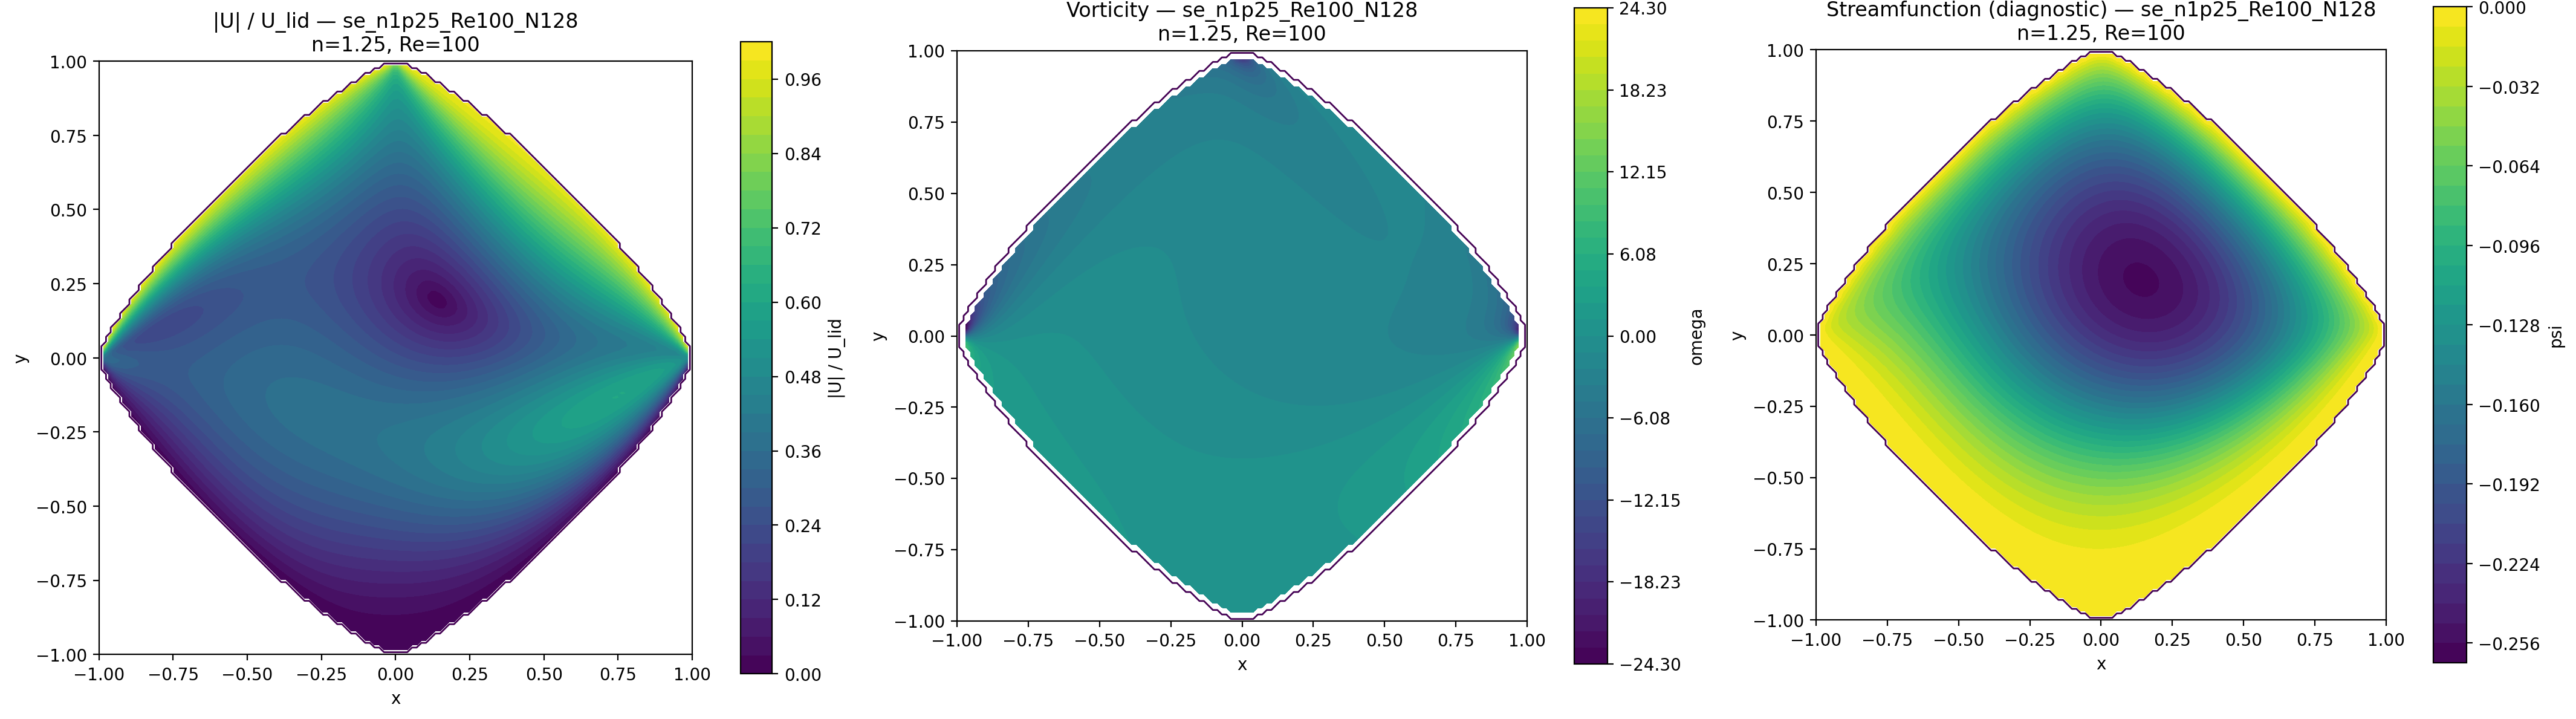
\includegraphics[width=\textwidth]{se_n1p25_Re100_N128_fields.png}
\caption{$n=1.25,\;Re=100$}
\end{subfigure}
\hfill
\begin{subfigure}[b]{0.32\textwidth}
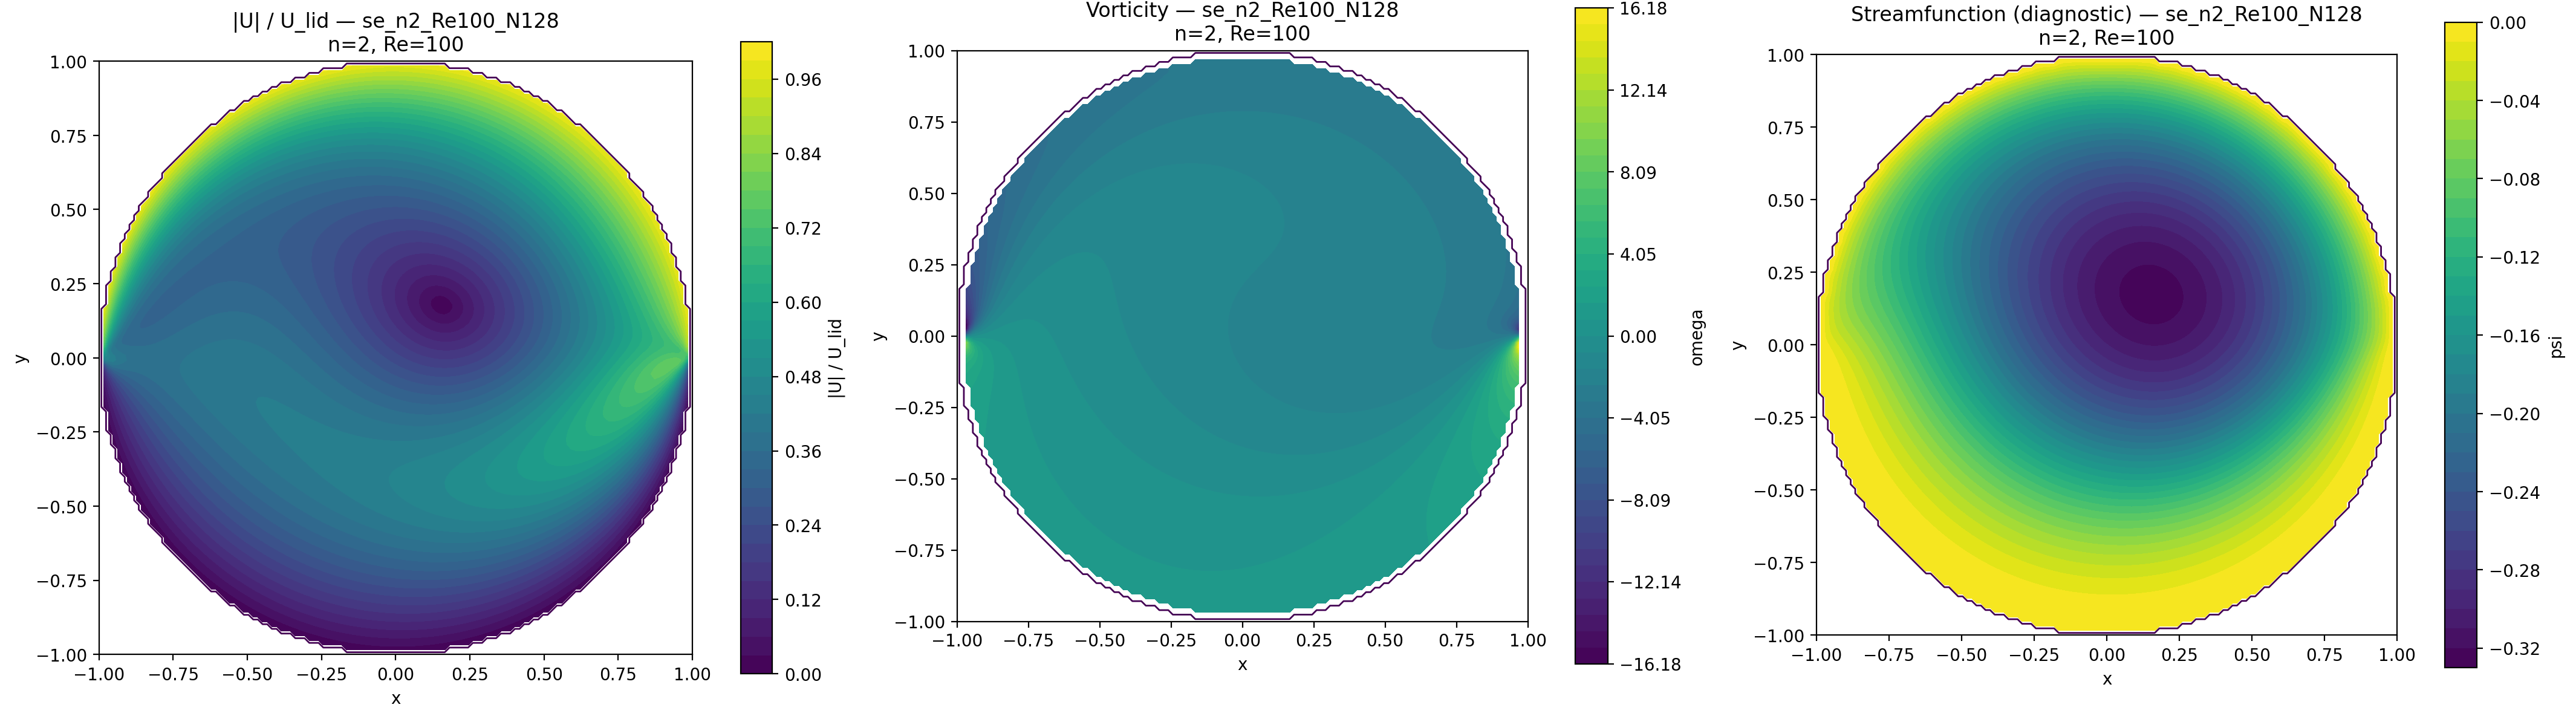
\includegraphics[width=\textwidth]{se_n2p0_Re100_N128_fields.png}
\caption{$n=2,\;Re=100$}
\end{subfigure}
\hfill
\begin{subfigure}[b]{0.32\textwidth}
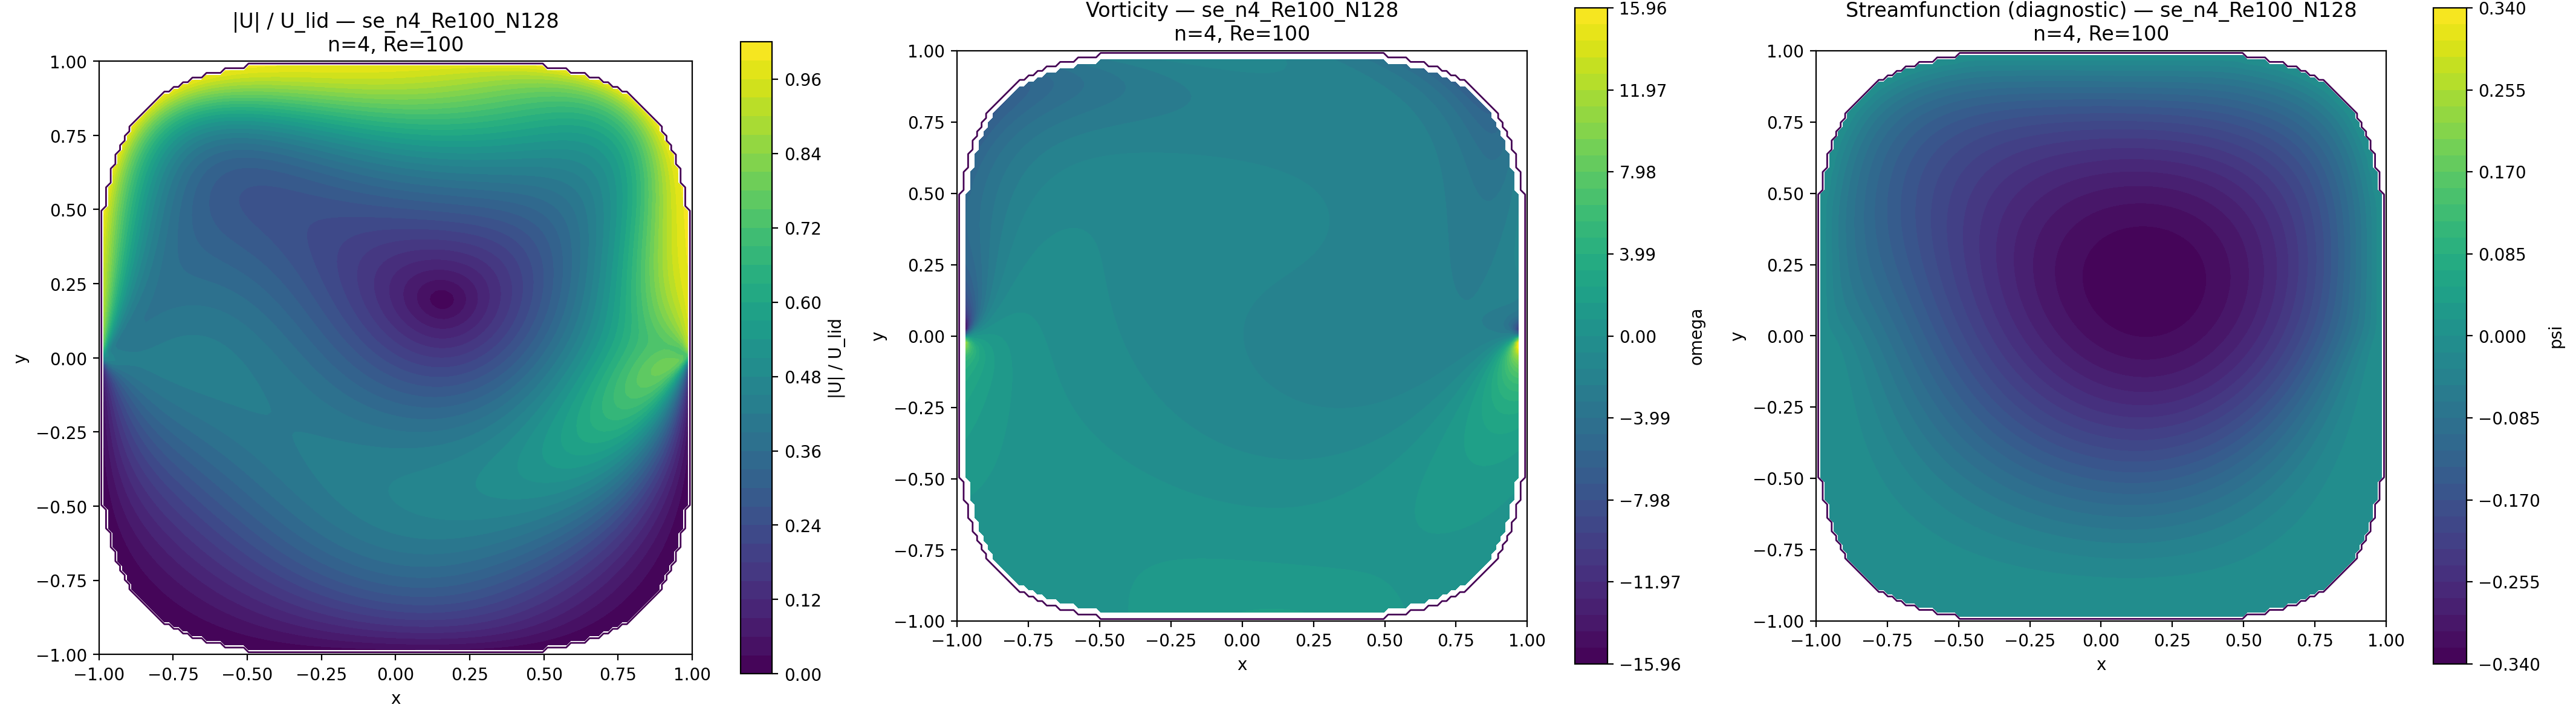
\includegraphics[width=\textwidth]{se_n4p0_Re100_N128_fields.png}
\caption{$n=4,\;Re=100$}
\end{subfigure}
\caption{Reference LBM velocity and streamfunction fields at $Re=100$ for representative geometry exponents.}
\color{blue}
\alttext{Reference LBM velocity and streamfunction fields at $Re=100$ for representative geometry exponents.}



\label{fig:atlas100}
\color{black}
\end{figure}

\color{blue}

\begin{table}[H]
\color{black}
\centering
\color{blue}
\caption{Complete $N=128$ grid of the area-normalized kinetic energy $KE/A$
and area-normalized dissipation $D/A$ in the mechanical convention of
Table~\ref{tab:energy30}. $KE/A$ uses the exact cavity area $A(n)$; $D/A$ uses
the area $A_{\rm mask}(n)$ of the discrete integration mask that carries the
sum defining $D$. Rows are geometry exponents and columns Reynolds numbers.
The absolute levels are resolution-sensitive; the table is used for geometry
ordering at fixed resolution only.}
\alttext{Complete $N=128$ grid of the area-normalized kinetic energy $KE/A$ and area-normalized dissipation $D/A$ in the mechanical convention of Table~. $KE/A$ uses the exact cavity area $A(n)$; $D/A$ uses the area $A_{\rm mask}(n)$ of the discrete integration mask that carries the sum defining $D$. Rows are geometry exponents and columns Reynolds numbers. The absolute levels are resolution-sensitive; the table is used for geometry ordering at fixed resolution only.}



\label{tab:grid190}
\scriptsize
\setlength{\tabcolsep}{3.0pt}
\tabbox{%
\begin{tabular}{@{}lrrrrrrrrrrrrrrrrrrr@{}}
\toprule
$n$ & 100 & 150 & 200 & 250 & 300 & 350 & 400 & 450 & 500 & 550 & 600 & 650 & 700 & 750 & 800 & 850 & 900 & 950 & 1000 \\
\midrule
\multicolumn{20}{l}{\bfseries $KE/A$}\\
1.25 & 0.0915 & 0.0936 & 0.0951 & 0.0962 & 0.0971 & 0.0978 & 0.0984 & 0.0989 & 0.0993 & 0.0996 & 0.0999 & 0.1002 & 0.1004 & 0.1006 & 0.1008 & 0.1010 & 0.1011 & 0.1013 & 0.1014 \\
1.5 & 0.0994 & 0.1018 & 0.1035 & 0.1047 & 0.1057 & 0.1065 & 0.1071 & 0.1077 & 0.1081 & 0.1086 & 0.1089 & 0.1093 & 0.1096 & 0.1099 & 0.1101 & 0.1104 & 0.1106 & 0.1109 & 0.1111 \\
1.75 & 0.1039 & 0.1064 & 0.1081 & 0.1094 & 0.1104 & 0.1112 & 0.1119 & 0.1125 & 0.1130 & 0.1134 & 0.1139 & 0.1142 & 0.1146 & 0.1149 & 0.1152 & 0.1155 & 0.1158 & 0.1161 & 0.1164 \\
2 & 0.1055 & 0.1080 & 0.1097 & 0.1110 & 0.1120 & 0.1128 & 0.1135 & 0.1141 & 0.1147 & 0.1151 & 0.1156 & 0.1160 & 0.1163 & 0.1167 & 0.1170 & 0.1173 & 0.1176 & 0.1179 & 0.1182 \\
2.5 & 0.1057 & 0.1082 & 0.1099 & 0.1111 & 0.1121 & 0.1129 & 0.1135 & 0.1141 & 0.1146 & 0.1150 & 0.1154 & 0.1158 & 0.1162 & 0.1165 & 0.1168 & 0.1171 & 0.1174 & 0.1176 & 0.1179 \\
3 & 0.1038 & 0.1063 & 0.1080 & 0.1092 & 0.1101 & 0.1109 & 0.1115 & 0.1121 & 0.1126 & 0.1130 & 0.1134 & 0.1138 & 0.1141 & 0.1144 & 0.1147 & 0.1150 & 0.1152 & 0.1155 & 0.1158 \\
4 & 0.1006 & 0.1031 & 0.1048 & 0.1060 & 0.1070 & 0.1077 & 0.1084 & 0.1089 & 0.1094 & 0.1099 & 0.1103 & 0.1107 & 0.1110 & 0.1114 & 0.1117 & 0.1120 & 0.1123 & 0.1126 & 0.1129 \\
5 & 0.0981 & 0.1007 & 0.1025 & 0.1038 & 0.1047 & 0.1055 & 0.1062 & 0.1068 & 0.1073 & 0.1078 & 0.1082 & 0.1086 & 0.1090 & 0.1093 & 0.1097 & 0.1100 & 0.1103 & 0.1106 & 0.1109 \\
6 & 0.0962 & 0.0989 & 0.1007 & 0.1021 & 0.1031 & 0.1039 & 0.1046 & 0.1052 & 0.1057 & 0.1062 & 0.1066 & 0.1070 & 0.1074 & 0.1077 & 0.1081 & 0.1084 & 0.1087 & 0.1090 & 0.1092 \\
8 & 0.0938 & 0.0966 & 0.0985 & 0.0999 & 0.1010 & 0.1019 & 0.1027 & 0.1033 & 0.1039 & 0.1044 & 0.1048 & 0.1052 & 0.1056 & 0.1060 & 0.1063 & 0.1066 & 0.1070 & 0.1072 & 0.1075 \\
\midrule
\multicolumn{20}{l}{\bfseries $D/A$}\\
1.25 & 0.07959 & 0.05743 & 0.04593 & 0.03877 & 0.03382 & 0.03016 & 0.02733 & 0.02507 & 0.02321 & 0.02165 & 0.02032 & 0.01917 & 0.01816 & 0.01727 & 0.01648 & 0.01576 & 0.01512 & 0.01454 & 0.01400 \\
 1.5 & 0.05360 & 0.03988 & 0.03255 & 0.02787 & 0.02458 & 0.02212 & 0.02019 & 0.01862 & 0.01733 & 0.01623 & 0.01529 & 0.01447 & 0.01375 & 0.01311 & 0.01254 & 0.01202 & 0.01155 & 0.01112 & 0.01073 \\
1.75 & 0.04320 & 0.03266 & 0.02692 & 0.02322 & 0.02060 & 0.01861 & 0.01705 & 0.01577 & 0.01471 & 0.01381 & 0.01304 & 0.01236 & 0.01176 & 0.01123 & 0.01075 & 0.01032 & 0.00992 & 0.00957 & 0.00924 \\
   2 & 0.03814 & 0.02903 & 0.02404 & 0.02080 & 0.01848 & 0.01673 & 0.01534 & 0.01421 & 0.01326 & 0.01246 & 0.01177 & 0.01116 & 0.01062 & 0.01014 & 0.00972 & 0.00933 & 0.00897 & 0.00865 & 0.00835 \\
 2.5 & 0.03421 & 0.02613 & 0.02168 & 0.01878 & 0.01671 & 0.01513 & 0.01388 & 0.01286 & 0.01201 & 0.01128 & 0.01066 & 0.01011 & 0.00962 & 0.00919 & 0.00880 & 0.00845 & 0.00813 & 0.00784 & 0.00757 \\
   3 & 0.03335 & 0.02541 & 0.02104 & 0.01820 & 0.01617 & 0.01462 & 0.01340 & 0.01241 & 0.01157 & 0.01087 & 0.01025 & 0.00972 & 0.00925 & 0.00883 & 0.00845 & 0.00811 & 0.00780 & 0.00751 & 0.00725 \\
   4 & 0.03412 & 0.02579 & 0.02124 & 0.01829 & 0.01620 & 0.01461 & 0.01336 & 0.01235 & 0.01150 & 0.01078 & 0.01016 & 0.00962 & 0.00915 & 0.00872 & 0.00834 & 0.00800 & 0.00769 & 0.00740 & 0.00714 \\
   5 & 0.03571 & 0.02678 & 0.02194 & 0.01883 & 0.01663 & 0.01497 & 0.01366 & 0.01260 & 0.01172 & 0.01098 & 0.01033 & 0.00978 & 0.00928 & 0.00885 & 0.00846 & 0.00811 & 0.00779 & 0.00750 & 0.00723 \\
   6 & 0.03739 & 0.02784 & 0.02271 & 0.01942 & 0.01710 & 0.01536 & 0.01400 & 0.01289 & 0.01197 & 0.01120 & 0.01054 & 0.00996 & 0.00945 & 0.00900 & 0.00860 & 0.00823 & 0.00790 & 0.00760 & 0.00733 \\
   8 & 0.04047 & 0.02981 & 0.02414 & 0.02053 & 0.01801 & 0.01612 & 0.01465 & 0.01346 & 0.01248 & 0.01165 & 0.01094 & 0.01033 & 0.00979 & 0.00931 & 0.00888 & 0.00850 & 0.00815 & 0.00784 & 0.00755 \\
\bottomrule
\end{tabular}}
\color{black}
\end{table}

\color{blue}
\section{Wall-curvature diagnostic}
\label{sec:curvature}
\color{black}

\color{blue}
The wall-curvature diagnostic interpolates the full periodic arclength table,
uses periodic central differences for the tangent angle and a wrapped angular
difference for the window curvature
\begin{equation}
  \kappa_w(s)=\frac{\operatorname{wrap}\left[\phi(s+w/2)-\phi(s-w/2)\right]}{w},
  \qquad w=0.05L_c .
  \label{eq:kappa_window}
\end{equation}
The sharp-set threshold is
$\kappa_w\geq2\langle|\kappa|\rangle_\Gamma$. All $190$ curvature rows were
recomputed from the archived fields; $D$, $A_{\rm mask}$, $D/A_{\rm mask}$ and
the curvature-independent wall-band fractions are unchanged.

\begin{table}[H]
\color{black}
\centering
\color{blue}
\caption{Analytical circle test. For $n=2$, $a=b=1$, the boundary is the unit
circle and the exact curvature is $\kappa=1$ everywhere.}
\alttext{Analytical circle test. For $n=2$, $a=b=1$, the boundary is the unit circle and the exact curvature is $\kappa=1$ everywhere.}



\label{tab:circle}
\tabbox{\begin{tabular}{@{}rrrrr@{}}
\toprule
$n_{\rm samples}$ & $w/L_c$ & $\kappa_{w,\max}$ & $\kappa_{w,\rm rms}$ & $f_{\rm sharp}$ \\
\midrule
2\,000  & 0.01 & 1.000000 & 1.000000 & 0.000 \\
2\,000  & 0.05 & 1.000000 & 1.000000 & 0.000 \\
5\,000  & 0.05 & 1.000000 & 1.000000 & 0.000 \\
20\,000 & 0.05 & 1.000000 & 1.000000 & 0.000 \\
50\,000 & 0.10 & 1.000000 & 1.000000 & 0.000 \\
\bottomrule
\end{tabular}}
\color{black}
\end{table}

\color{blue}
\begin{table}[H]
\color{black}
\centering
\color{blue}
\caption{Geometry-only curvature metrics (independent of $Re$).}
\alttext{Geometry-only curvature metrics (independent of $Re$).}



\label{tab:curvgeom}
\tabbox{\begin{tabular}{@{}crrrr@{}}
\toprule
$n$ & $\kappa_{w,\max}$ & $\kappa_{w,\rm rms}$ & $f_{\rm sharp}$ & $\langle|\kappa|\rangle_\Gamma$ \\
\midrule
1.25 & 8.726 & 2.294 & 0.082 & 1.091 \\
1.50 & 4.394 & 1.393 & 0.084 & 1.058 \\
1.75 & 2.109 & 1.077 & 0.033 & 1.027 \\
2.00 & 1.000 & 1.000 & 0.000 & 1.000 \\
2.50 & 1.397 & 1.023 & 0.000 & 0.960 \\
3.00 & 1.775 & 1.087 & 0.000 & 0.932 \\
4.00 & 2.498 & 1.221 & 0.207 & 0.895 \\
5.00 & 3.192 & 1.345 & 0.215 & 0.873 \\
6.00 & 3.861 & 1.458 & 0.207 & 0.859 \\
8.00 & 5.125 & 1.655 & 0.186 & 0.840 \\
\bottomrule
\end{tabular}}
\end{table}
\color{black}

\color{blue}
The corrected maximum curvature is minimal at the circle and rises both at
sharp tips ($n<2$) and near-square corners ($n>2$), as expected geometrically.
The sharp set is empty for $n=2,2.5,3$ and non-empty at both ends of the family.

\begin{table}[H]
\centering
\caption{Correlations with $D/A_{\rm mask}$ at fixed $Re$. Spearman values
are shown only for $Re=1000$.}
\alttext{Correlations with $D/A_{\rm mask}$ at fixed $Re$. Spearman values are shown only for $Re=1000$.}



\label{tab:currcorr}
\tabbox{\begin{tabular}{@{}lcccc@{}}
\toprule
predictor & $Re=100$, $r$ & $Re=500$, $r$ & $Re=1000$, $r$ & $Re=1000$, $\rho$ \\
\midrule
$\kappa_{w,\rm rms}$ & $+0.834$ & $+0.748$ & $+0.709$ & $+0.115$ \\
$\langle\kappa\rangle_D$ & $+0.667$ & $+0.462$ & $+0.385$ & $+0.636$ \\
$f_{\rm sharp}$ & $+0.794$ & $-0.068$ & $-0.238$ & $-0.472$ \\
$f_{0.025}$ & $+0.795$ & $+0.852$ & $+0.848$ & $+0.794$ \\
\bottomrule
\end{tabular}}
\end{table}
\color{black}

\color{blue}
At fixed $Re$, RMS window curvature remains positively correlated with
$D/A_{\rm mask}$, but the Pearson coefficient decreases from $+0.834$ at
$Re=100$ to $+0.709$ at $Re=1000$ and the Spearman coefficient at $Re=1000$
is only $+0.115$. The sharp-set fraction is negatively correlated at $Re=500$
and $Re=1000$. These results do not support wall curvature alone as the
control on the $D/A_{\rm mask}$ minimum.

\begin{figure}[H]
\centering
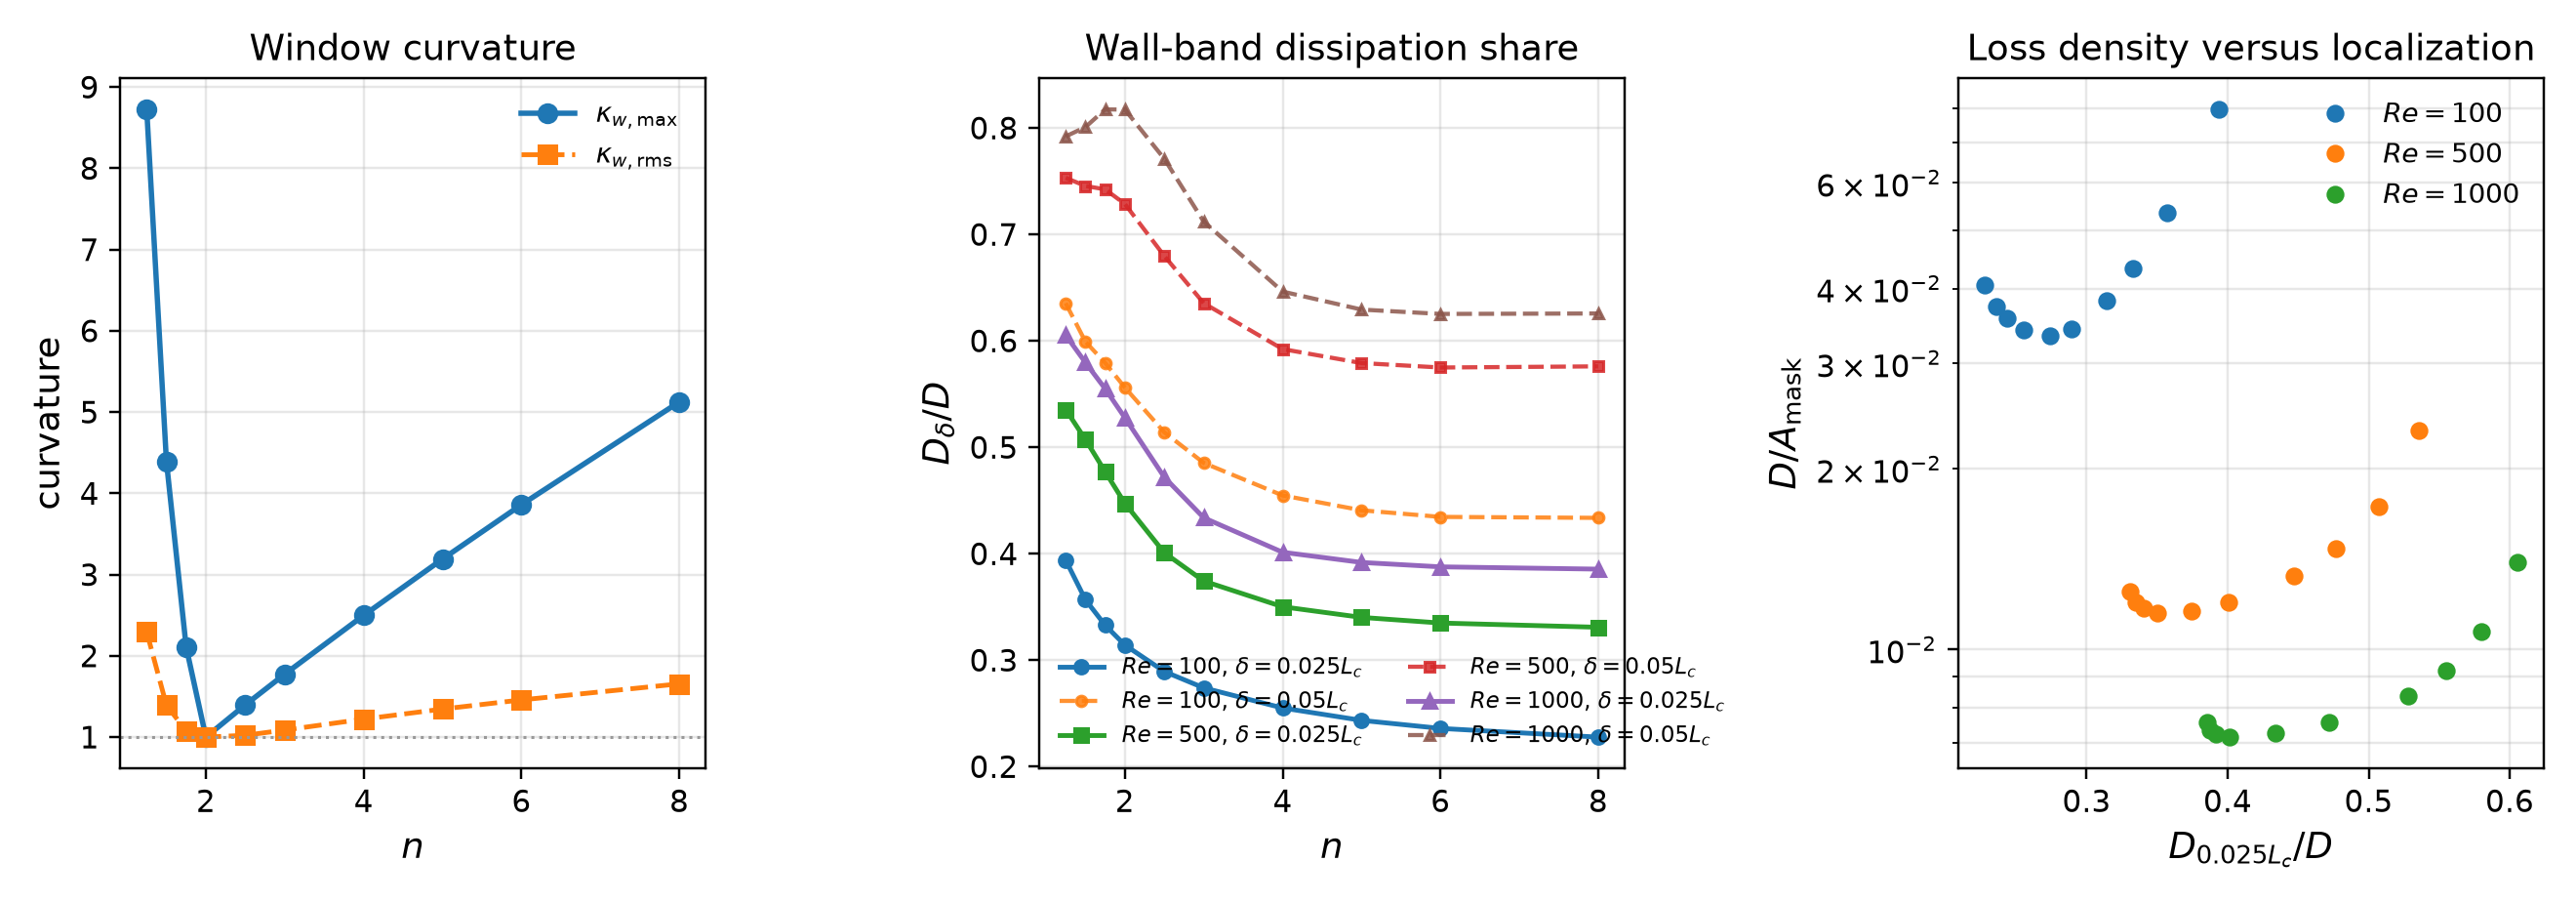
\includegraphics[width=0.96\textwidth]{fig_nearwall_large_axes.png}
\caption{Wall-curvature diagnostic, wall-band dissipation share and
$D/A_{\rm mask}$ versus wall-band localization on the reference grid. Axes and
tick labels are enlarged for review; the panels use the final periodic
arclength interpolation.}
\alttext{Wall-curvature diagnostic, wall-band dissipation share and $D/A_{\rm mask}$ versus wall-band localization on the reference grid. Axes and tick labels are enlarged for review; the panels use the final periodic arclength interpolation.}



\label{fig:nearwall_large}
\color{black}
\end{figure}

\color{blue}
\section{Extended additive wall/core budget}
\label{sec:corewall}
\color{black}

\color{blue}
For every case the same gradient-valid mask $M$ is partitioned into
$W_\delta=M\cap\{\operatorname{dist}(\mathbf{x},\Gamma)\leq\delta\}$ and
$C_\delta=M\setminus W_\delta$, with $\delta/L_c\in\{0.025,0.05\}$. Using the
same integrand as in Eq.~\eqref{eq:mech_factor},
\[
  \frac{D_{\rm mask}}{A_{\rm mask}}
  =\frac{D_{\rm wall}}{A_{\rm mask}}+\frac{D_{\rm core}}{A_{\rm mask}},
  \qquad A_{\rm mask}=N_M\Delta x^2 .
\]
There are $253$ archived cases and two band widths, hence $506$ rows. The
maximum absolute additivity residual over all rows is $2.78\times10^{-17}$.
\color{black}

\color{blue}
\begin{table}[H]
\color{black}
\centering
\color{blue}
\caption{Additive budget for the detailed case $Re=1000$, $N=256$,
$\delta=0.05L_c$. All denominators are $A_{\rm mask}$, never $A_{\rm core}$
or the exact geometric area.}
\alttext{Additive budget for the detailed case $Re=1000$, $N=256$, $\delta=0.05L_c$. All denominators are $A_{\rm mask}$, never $A_{\rm core}$ or the exact geometric area.}



\label{tab:budgetcase}
\tabbox{\begin{tabular}{@{}crrrr@{}}
\toprule
$n$ & $D/A_{\rm mask}$ & $D_{\rm wall}/A_{\rm mask}$ & $D_{\rm core}/A_{\rm mask}$ & $f_{\rm core}$ \\
\midrule
2 & 0.010289 & 0.008853 & 0.001437 & 14.0\% \\
3 & 0.008943 & 0.006941 & 0.002002 & 22.4\% \\
4 & 0.008797 & 0.006329 & 0.002468 & 28.1\% \\
6 & 0.008968 & 0.006235 & 0.002733 & 30.5\% \\
8 & 0.009199 & 0.006378 & 0.002821 & 30.7\% \\
\bottomrule
\end{tabular}
}
\color{black}
\end{table}

\color{blue}
\begin{figure}[H]
\color{black}
\centering
\color{blue}
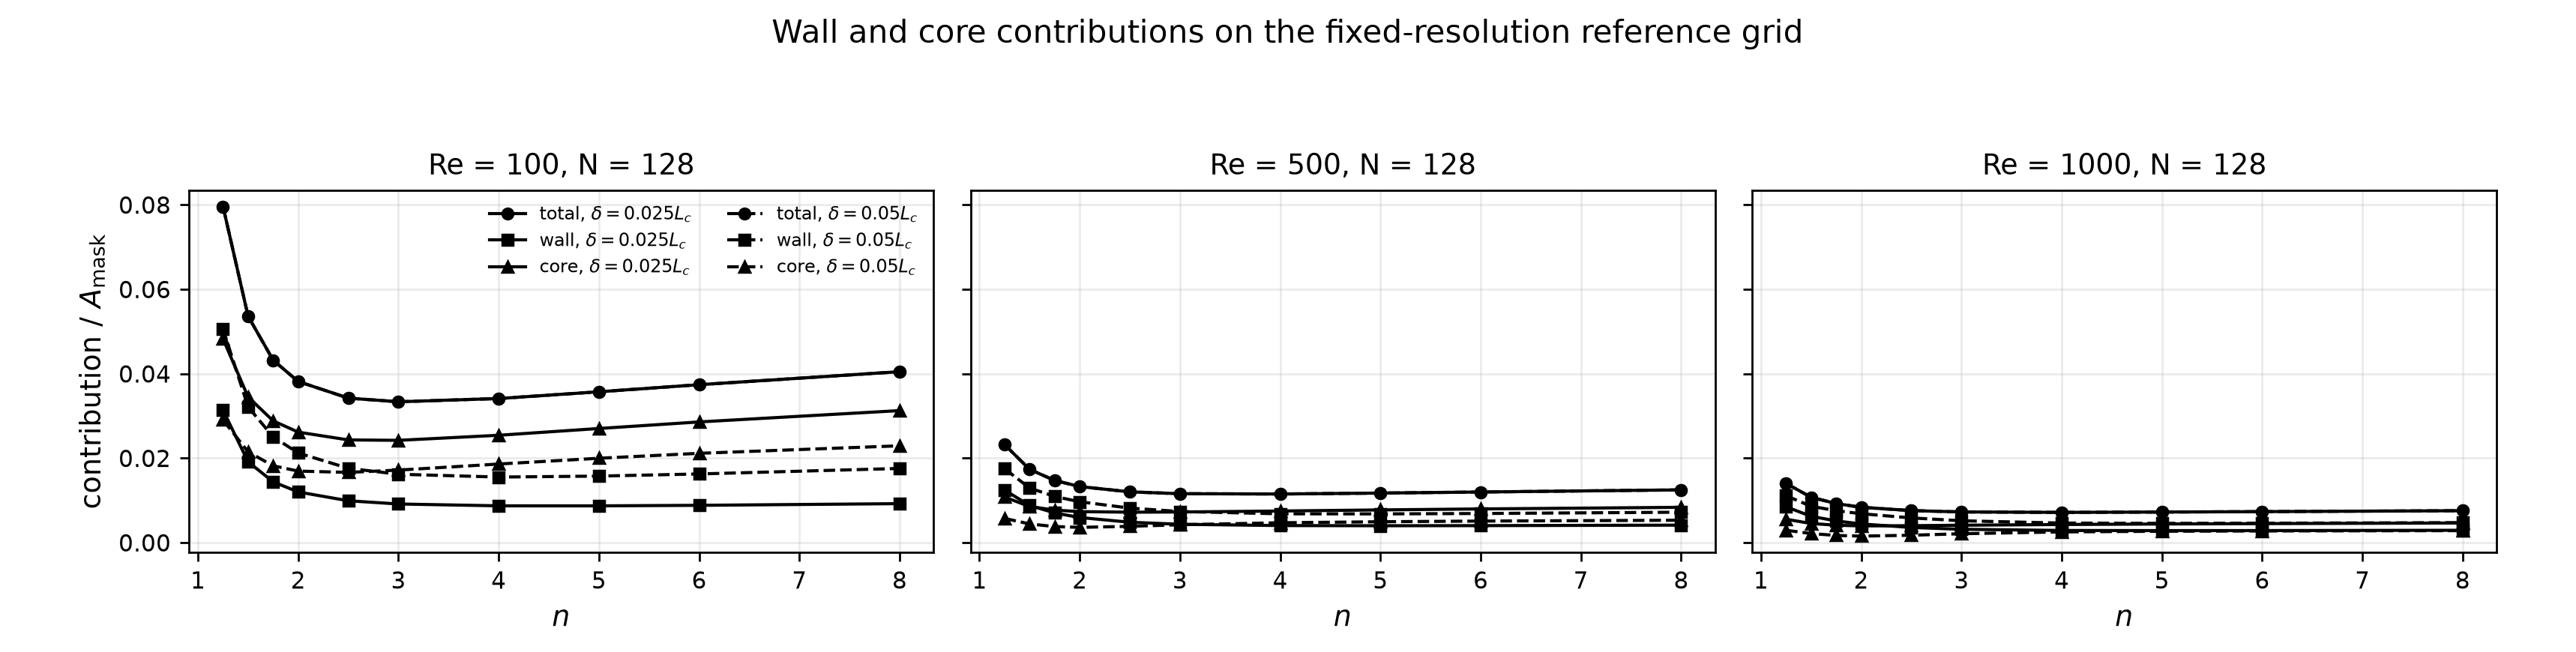
\includegraphics[width=0.94\textwidth]{fig_supp_corewall_Re100_500_1000.png}
\caption{Total, wall and core contributions divided by $A_{\rm mask}$ for
$N=128$, $Re=100,500,1000$. Solid lines use $\delta=0.025L_c$ and dashed
lines use $\delta=0.05L_c$.}
\alttext{Total, wall and core contributions divided by $A_{\rm mask}$ for $N=128$, $Re=100,500,1000$. Solid lines use $\delta=0.025L_c$ and dashed lines use $\delta=0.05L_c$.}



\label{fig:corewall}
\color{black}
\end{figure}

\color{blue}
Table~\ref{tab:budgetcase} gives the detailed target case. From $n=4$ to
$n=8$, $D/A_{\rm mask}$ rises by $0.000403$, of which $0.000353$ ($87.8\%$) is
the core contribution and $0.000049$ ($12.2\%$) is the wall contribution. The
$88\%$ number is the core share of the *increase*, not the core share of the
total dissipation. The latter is $28.1\%$ at $n=4$ and $30.7\%$ at $n=8$.
\color{black}

\color{blue}
\begin{table}[H]
\centering
\caption{Core share of the $n=4\to8$ increase wherever both exponents exist.
The $Re=100$, $N=256$ increment is unavailable because that campaign has no
$n=8$ field.}
\alttext{Core share of the $n=4\to8$ increase wherever both exponents exist. The $Re=100$, $N=256$ increment is unavailable because that campaign has no $n=8$ field.}
\color{black}

\color{blue}


\label{tab:budgetrange}
\tabbox{\begin{tabular}{@{}ccrrrr@{}}
\toprule
$N$ & $Re$ & $\delta/L_c$ & $\Delta(D/A)$ & $\Delta(D_{\rm core}/A)$ & core share \\
\midrule
128 & 100 & 0.025 & 0.006356 & 0.005841 & 91.9\% \\
128 & 100 & 0.05 & 0.006356 & 0.004319 & 67.9\% \\
128 & 500 & 0.025 & 0.000978 & 0.000876 & 89.6\% \\
128 & 500 & 0.05 & 0.000978 & 0.000601 & 61.5\% \\
128 & 1000 & 0.025 & 0.000404 & 0.000361 & 89.5\% \\
128 & 1000 & 0.05 & 0.000404 & 0.000298 & 73.8\% \\
256 & 500 & 0.025 & 0.000992 & 0.000921 & 92.9\% \\
256 & 500 & 0.05 & 0.000992 & 0.000657 & 66.3\% \\
256 & 1000 & 0.025 & 0.000402 & 0.000402 & 99.8\% \\
256 & 1000 & 0.05 & 0.000402 & 0.000353 & 87.8\% \\
\bottomrule
\end{tabular}
}
\color{black}
\end{table}

\color{blue}
Table~\ref{tab:budgetrange} qualifies the generalization. Across the ten
available $(N,Re,\delta)$ combinations the core share of the positive increment
lies between $61.5\%$ and $99.8\%$. The share depends on resolution, Reynolds
number and band thickness; no universal causal percentage is claimed. The
underlying $n$ grids are not uniform across campaigns, so comparisons are made
only where the same two exponents are present.

\section{Common-support LBM/FEM dissipation}
\label{sec:common_support}

The archived LBM fields store lid-normalized velocity
$\mathbf{u}=\mathbf{u}_{\rm LBM}/U_{\rm lid}$, with $U_{\rm lid}=0.05$ in the
original lattice simulation, on coordinates $x,y\in[-1,1]$ with $a=1$ and
$L_c=2$. In these paper units the viscosity is $\nu=U_{\rm lid}L_c/Re=2/Re$;
the value \texttt{nu\_lbm} stored in the archive is the corresponding lattice-unit
quantity. The LBM integrand used throughout the physics article is
\begin{equation}
  2\nu\,S:S = 2\nu\left(u_x^2+v_y^2+\tfrac12(u_y+v_x)^2\right)
            = \frac{2}{Re}\left(2u_x^2+2v_y^2+(u_y+v_x)^2\right),
  \label{eq:mech_factor}
\end{equation}
so the mechanical factor two in $D=2\int(2S:S/Re)\,dA$ is counted once. The
FEM form assembled from the P2 degrees of freedom is
$D_{\rm FEM}^{\Omega}=2\nu\int_\Omega S(\mathbf{u}_h):S(\mathbf{u}_h)\,dA$
with $U_{\rm lid}=1$ and the same $\nu=2/Re$. No additional velocity rescaling
or second factor two is applied.

The LBM value $D_{\rm LBM}^{M}$ uses central differences on the gradient-valid
mask $M$:
\begin{equation}
  M=\{\mathbf{x}_{jk}\in\Omega_{\rm fluid}^{\rm grid}:\;
      \mathbf{x}_{jk\pm1}\in\Omega_{\rm fluid}^{\rm grid}
      \text{ in both coordinate directions}\},
  \qquad
  D_{\rm LBM}^{M}=2\nu\sum_{k\in M}S_{k}:S_{k}\,\Delta x^2 .
  \label{eq:mask}
\end{equation}
For the same-support FEM value, each $k\in M$ is projected onto its containing
P2 element, the strain is evaluated from the element shape functions, and the
same lattice weight $\Delta x^2$ is used:
$D_{\rm FEM}^{M}=2\nu\sum_{k\in M}S_h(\mathbf{x}_k):S_h(\mathbf{x}_k)\Delta x^2$.
All $9\,488$--$15\,168$ masked nodes were covered by the $n_{\rm ref}=6$ mesh.

\begin{table}[H]
\color{black}
\centering
\color{blue}
\caption{Common-support dissipation at $N=128$ and $n_{\rm ref}=6$.
Here $\varepsilon_D=100|D_{\rm LBM}^{M}-D_{\rm FEM}^{M}|/D_{\rm FEM}^{M}$;
the last column is the same FEM strain integrated over the full P2 domain.}
\alttext{Common-support dissipation at $N=128$ and $n_{\rm ref}=6$. Here $\varepsilon_D=100|D_{\rm LBM}^{M}-D_{\rm FEM}^{M}|/D_{\rm FEM}^{M}$; the last column is the same FEM strain integrated over the full P2 domain.}



\label{tab:commonsupport}
\tabbox{\begin{tabular}{@{}ccrrrr@{}}
\toprule
$n$ & $Re$ & $D_{\rm LBM}^{M}$ & $D_{\rm FEM}^{M}$ & $\varepsilon_D$ (\%) & $D_{\rm FEM}^{\Omega}$ \\
\midrule
1.25 & 100 & 0.211656 & 0.200336 & 5.65 & 0.327424 \\
1.25 & 1000 & 0.035837 & 0.032877 & 9.00 & 0.062231 \\
2 & 100 & 0.117331 & 0.116496 & 0.72 & 0.224821 \\
2 & 1000 & 0.022538 & 0.024512 & 8.05 & 0.049404 \\
4 & 100 & 0.107158 & 0.121964 & 12.14 & 0.233612 \\
4 & 1000 & 0.020330 & 0.024620 & 17.42 & 0.050635 \\
8 & 100 & 0.127297 & 0.152335 & 16.44 & 0.267256 \\
8 & 1000 & 0.022126 & 0.027665 & 20.02 & 0.054848 \\
\bottomrule
\end{tabular}
}
\end{table}

\begin{figure}[H]
\centering
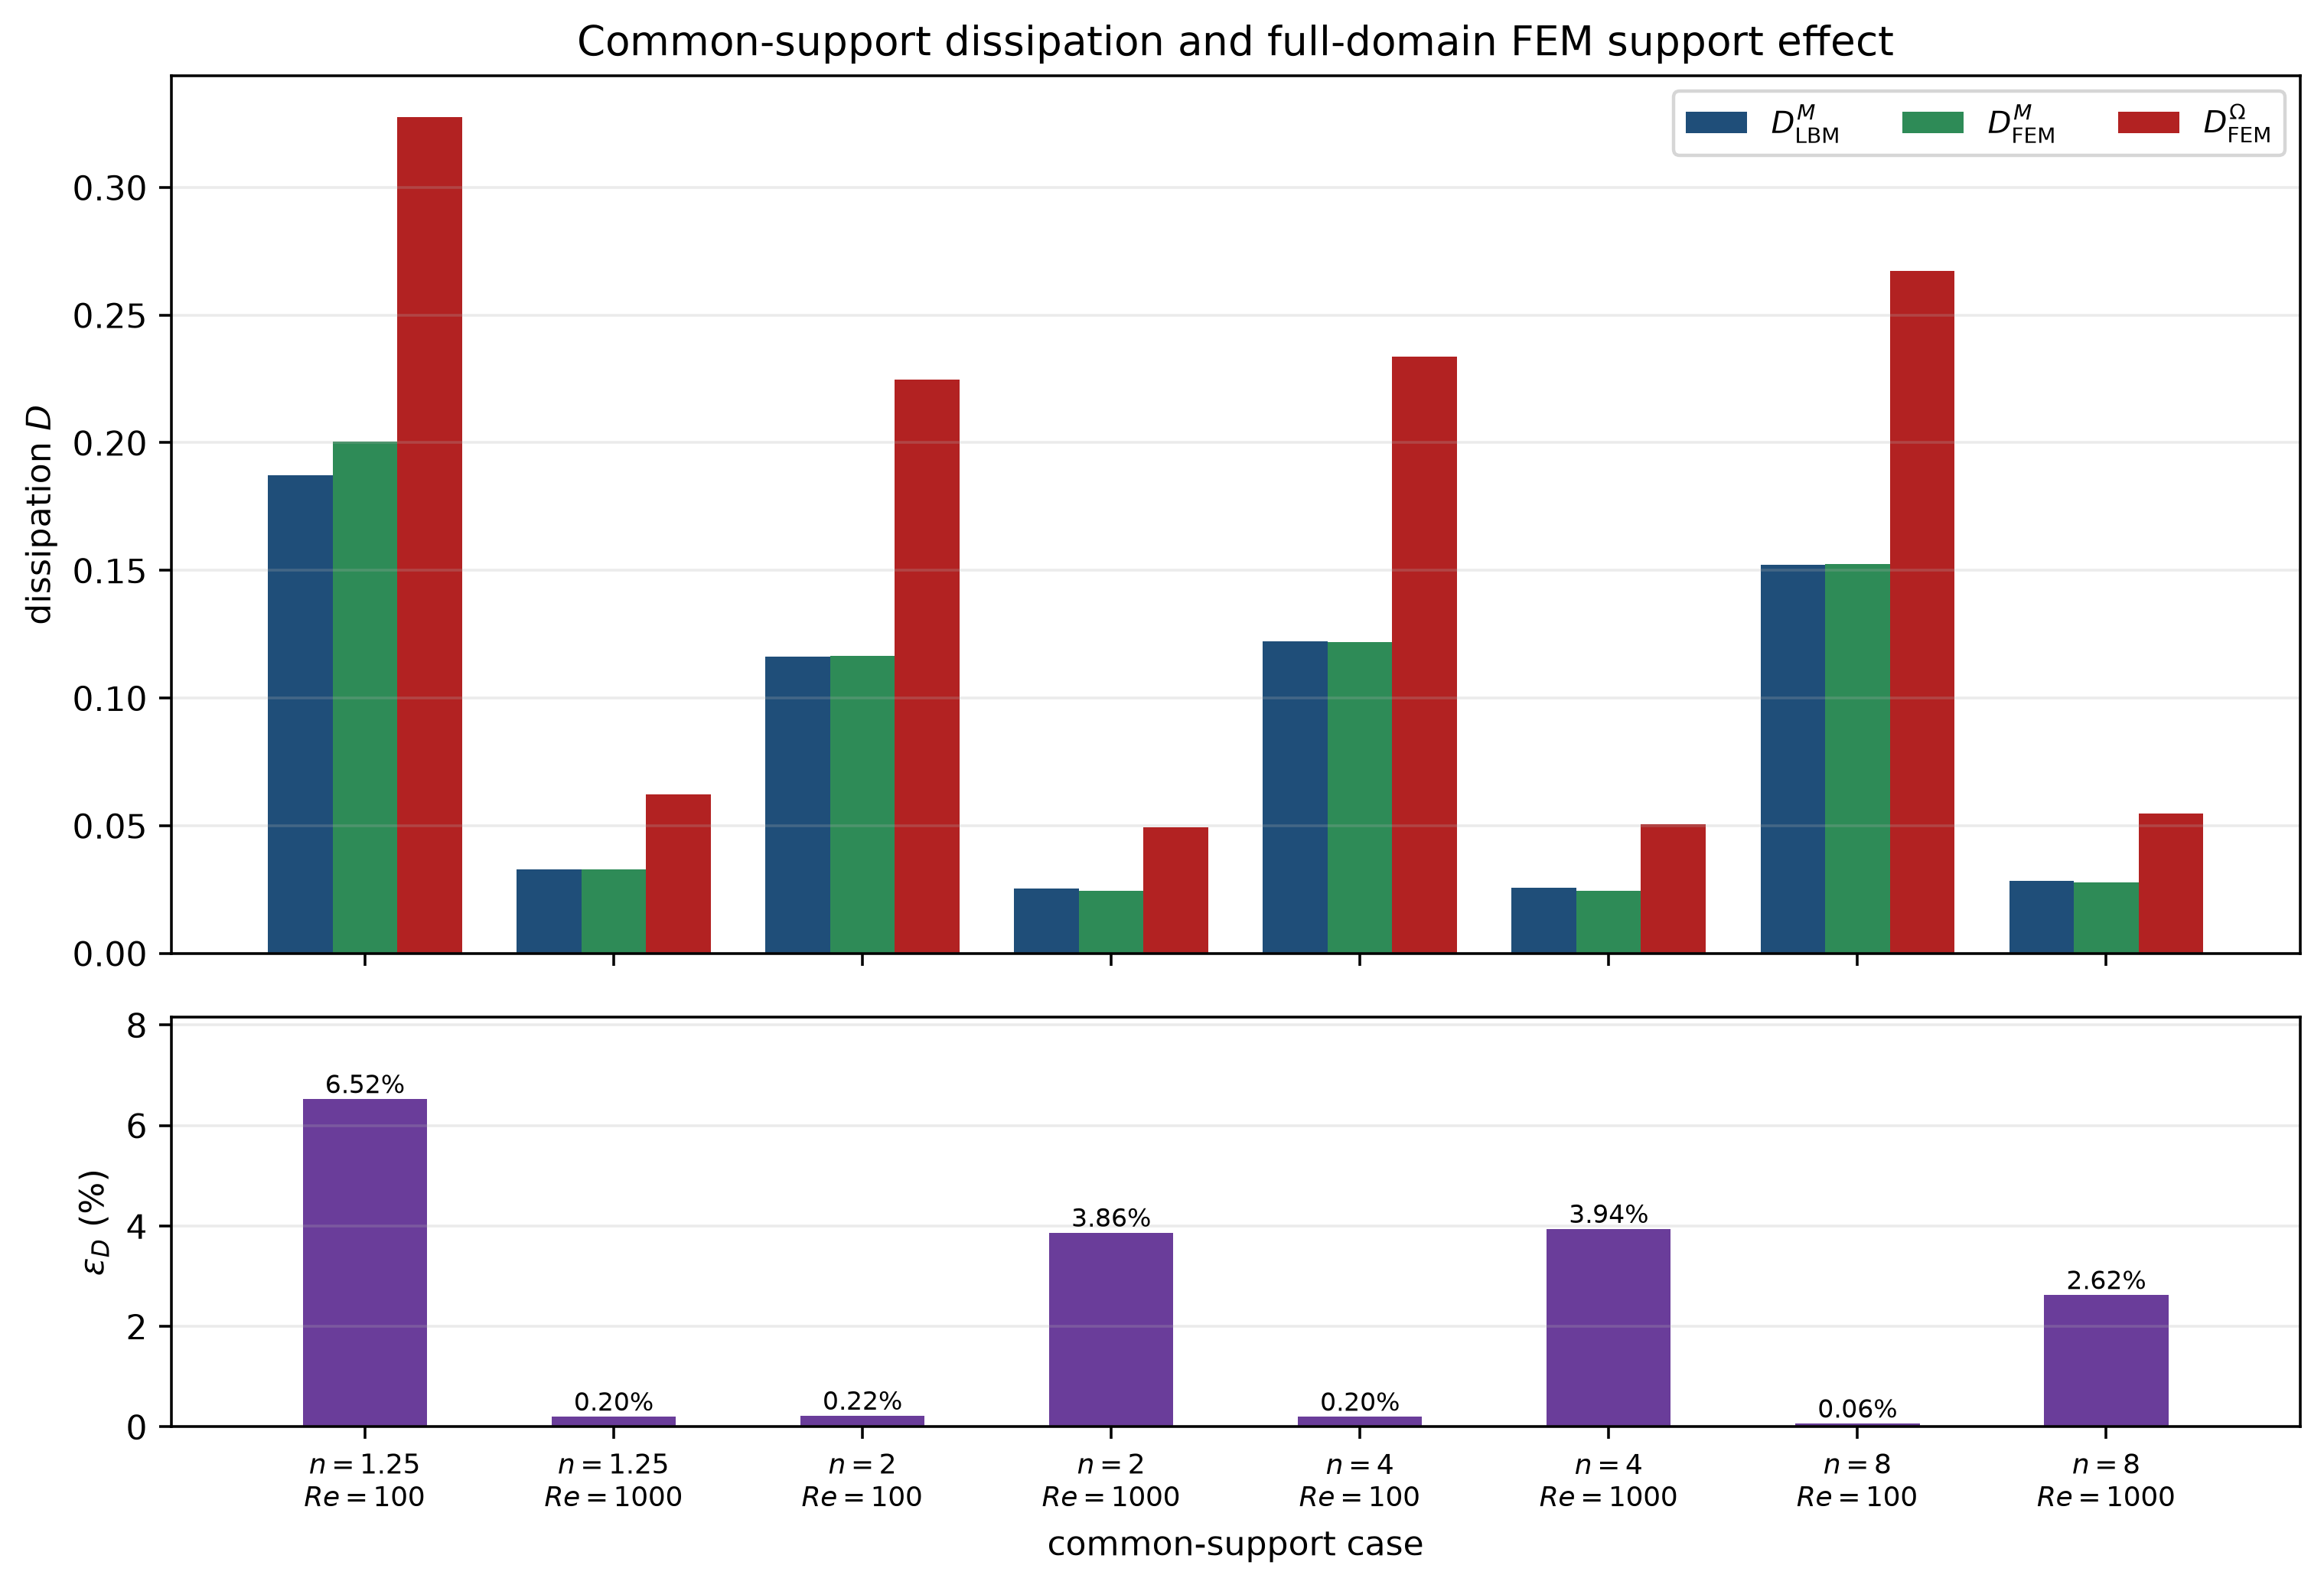
\includegraphics[width=0.88\textwidth]{fig_supp_common_support_dissipation.png}
\caption{Comparison of $D_{\rm LBM}^{M}$, $D_{\rm FEM}^{M}$ and
$D_{\rm FEM}^{\Omega}$ for the eight common-support cases. The difference
between the two FEM bars is a support effect, not a different velocity
normalization.}
\alttext{Comparison of $D_{\rm LBM}^{M}$, $D_{\rm FEM}^{M}$ and $D_{\rm FEM}^{\Omega}$ for the eight common-support cases. The difference between the two FEM bars is a support effect, not a different velocity normalization.}



\label{fig:commonsupport}
\color{black}
\end{figure}

\color{blue}
Table~\ref{tab:commonsupport} and Fig.~\ref{fig:commonsupport} show
$\varepsilon_D=0.72$--$20.02\%$, while
$D_{\rm FEM}^{\Omega}/D_{\rm FEM}^{M}=1.63$--$2.06$. The quantity labelled
``rel.\ $D$ error'' in the gradient-reconstruction table is
$|D_{\rm FD,lattice}-D_{\rm exact,lattice}|/D_{\rm exact,lattice}$: it compares
two gradient reconstructions at lattice points sampled from a saved FEM field,
and is not an LBM/FEM validation error. The closest common-support agreement
occurs at $n=2$, $Re=100$; the discrepancy grows for sharper or nearly square
geometries at higher $Re$. These values are a same-support comparison, not a
grid-converged absolute validation.

\section{FEM mesh, iteration and junction audit}
\label{sec:fem_audit}

The independent solver is a Taylor--Hood P2/P1 Navier--Stokes implementation.
The saddled system is assembled with $\nu=U_{\rm lid}L_c/Re$ and solved by
Picard iteration with relaxation $1$ and a relative $L_2$ velocity tolerance
$10^{-9}$. The new verification ladder used $U_{\rm lid}=1$, $a=1$,
$\nu=2/Re$, quadrature order $4$, $n\in\{1.25,2,4,8\}$,
$Re\in\{100,400,1000\}$ and $n_{\rm ref}\in\{4,5,6\}$: $12$ cases and $36$
solves. All $36$ solves converged in $14$--$34$ iterations.

\begin{table}[H]
\centering
\caption{Taylor--Hood mesh levels used in the verification ladder. The total
unknown count is $2(V+E)+V$: vector P2 velocity plus scalar P1 pressure.}
\alttext{Taylor--Hood mesh levels used in the verification ladder. The total unknown count is $2(V+E)+V$: vector P2 velocity plus scalar P1 pressure.}
\color{black}



\color{blue}
\label{tab:femmesh}
\tabbox{\begin{tabular}{@{}rrrrr@{}}
\toprule
$n_{\rm ref}$ & vertices $V$ & triangles $T$ & velocity DOFs & total unknowns \\
\midrule
4 & 545  & 1\,024  & 4\,226  & 4\,771  \\
5 & 2\,113 & 4\,096  & 16\,642 & 18\,755 \\
6 & 8\,321 & 16\,384 & 66\,050 & 74\,371 \\
\bottomrule
\end{tabular}}
\end{table}
\color{black}

\color{blue}
The Dirichlet assignment is nodal and discontinuous. For every boundary
velocity degree of freedom, the FEM code evaluates $y>0$ and imposes
$U_{\rm lid}(m_y,-m_x)$ if true and $\mathbf{0}$ otherwise; there is no
interpolation or regularization length. The same strict label is used for LBM
boundary links. The radial mesh retains cardinal nodes at $(\pm1,0)$ to
machine precision. A runtime check on the executed meshes gives:

\begin{itemize}
  \item right junction $(+1,0)$: $y=0$ exactly, assigned to the fixed wall;
  \item left junction $(-1,0)$: $y=+1.22\times10^{-16}$, assigned to the
        moving wall by the strict $y>0$ test.
\end{itemize}

\begin{figure}[H]
\centering
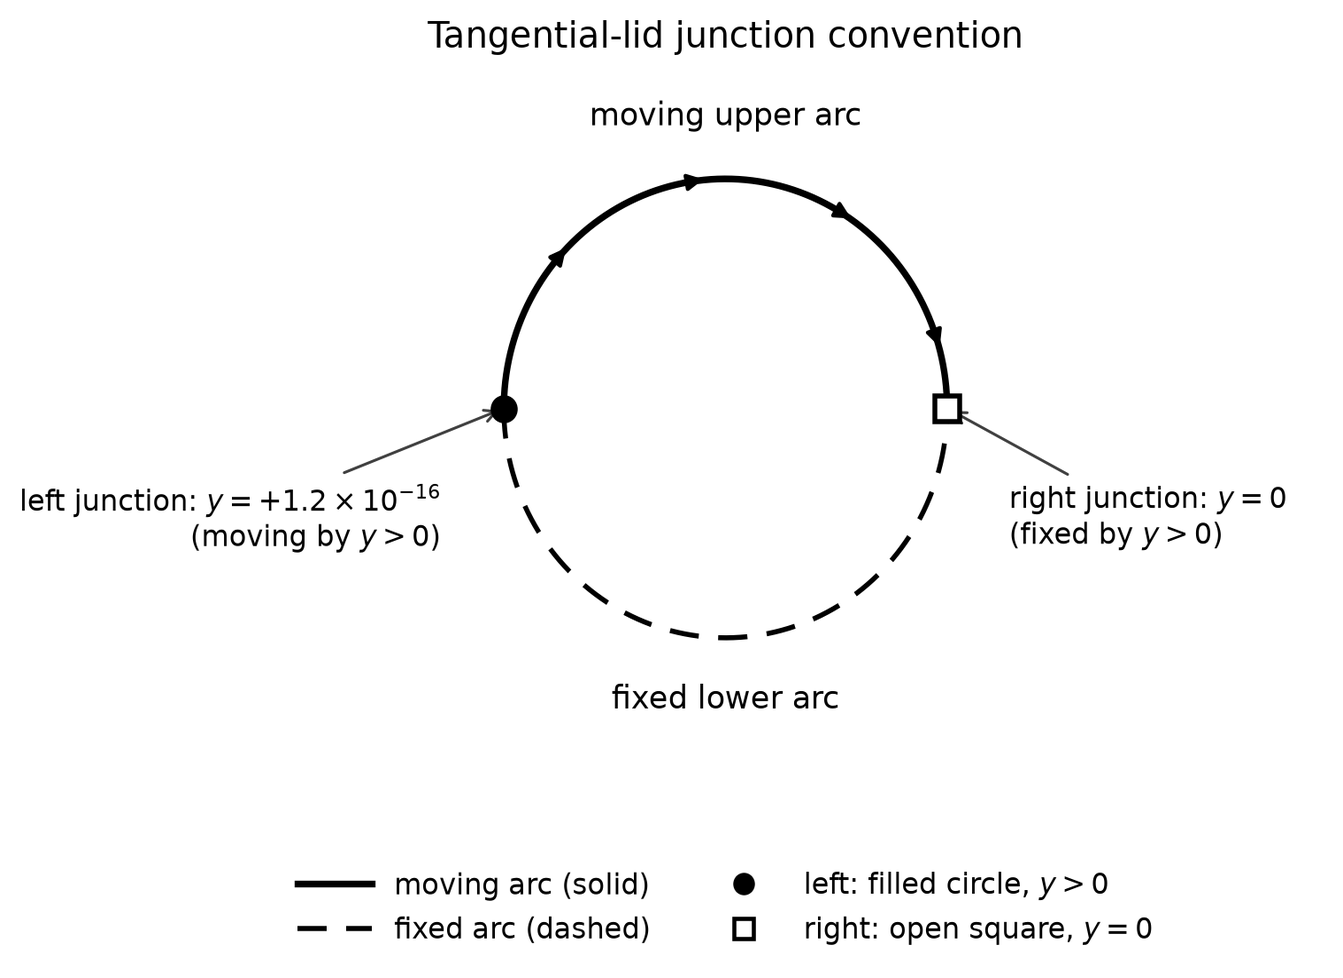
\includegraphics[width=0.72\textwidth]{fig_supp_fem_junction_schematic.png}
\caption{Tangential-lid junction convention. The upper arc is moving and the
lower arc is fixed. The two junctions are points of velocity discontinuity;
the FEM assignment is by a strict nodal $y>0$ test, without blending.}
\alttext{Tangential-lid junction convention. The upper arc is moving and the lower arc is fixed. The two junctions are points of velocity discontinuity; the FEM assignment is by a strict nodal $y>0$ test, without blending.}
\color{black}



\color{blue}
\label{fig:femjunction_supp}
\end{figure}

This machine-precision asymmetry (Fig.~\ref{fig:femjunction_supp}) is a
discrete implementation detail, not a physical regularization. The FEM junction
contribution is therefore mesh-sensitive in the same way as the LBM junction
diagnostic. Direct 5-to-6 mesh changes in $D_{\rm FEM}$ are $1.32\%$--$8.46\%$;
they are reported as mesh sensitivity only, with no Richardson extrapolation.

\section{Energy identity, pressure convention and archived-field diagnostic}
\label{sec:energy}

Three distinct statements must not be confused.

\begin{enumerate}
  \item \emph{Continuous identity.} For a smooth incompressible Newtonian
        velocity and pressure,
        \[
          \nabla\cdot\left[\left(\tfrac12|\mathbf{u}|^2+p\right)\mathbf{u}
          -2\nu S\mathbf{u}\right]=-2\nu S:S .
        \]
        This is an analytical statement and is not what the archived-field test
        verifies.
  \item \emph{Exact discrete LBM balance.} The collision--streaming scheme has
        its own discrete momentum and energy bookkeeping. That exact discrete
        balance was not reconstructed from the saved macroscopic fields.
  \item \emph{Archived-field diagnostic.} Central differences were applied to
        the saved $(\rho,\mathbf{u})$ pair on the gradient-valid mask, with
        pressure and interface fluxes evaluated on artificial circular cuts.
        This is the only quantity tested here, and it does not close.
\end{enumerate}

In the LBM archive the pressure convention is
$p_{\rm LBM}=c_s^2(\rho_{\rm LBM}-1)$ with $c_s^2=1/3$. Since the stored
velocities are lid-normalized with $U_{\rm lid}=0.05$, the pressure entering
the paper-unit diagnostic is
$p=(\rho-1)/(3U_{\rm lid}^2)$. For $n=4$, $Re=1000$, the diagnostic gives
\begin{equation}
  \frac{\int_{\partial\Omega_{\rm art}}
        \left[(\tfrac12|\mathbf{u}|^2+p)\mathbf{u}-2\nu S\mathbf{u}\right]\cdot\mathbf{n}\,ds}
       {-\int_{\Omega_{\rm exc}}2\nu S:S\,dA}
  =-4.419 ,
  \label{eq:flux_ratio}
\end{equation}
instead of $+1$. Equivalently, the pressure coefficient needed to close the
archived-field flux is $-0.0783$ instead of $+1$. The likely contributors are
the weakly compressible LBM pressure field, finite-difference gradients on a
near-wall mask and interpolation on the artificial cuts. No empirical pressure
rescaling is applied. No global power-balance closure is claimed, and the
interface flux is retained only as an unverified diagnostic.

\section{Moving-wall length and lid-power assessment}
\label{sec:lidpower}

The moving lid is the whole upper arc of $|x|^n+|y|^n=1$. With $p=2/n$ and
$\theta\in[0,\pi/2]$,
\begin{equation}
  x=\cos^p\theta,\qquad y=\sin^p\theta,\qquad
  L_{\rm mov}=2\int_0^{\pi/2}
  p\sqrt{\cos^{2p-2}\theta\,\sin^2\theta+
        \sin^{2p-2}\theta\,\cos^2\theta}\,d\theta .
  \label{eq:lmov}
\end{equation}
The integral has integrable algebraic endpoint singularities for $n>2$;
an independent Cartesian quadrature with $t=1-u^n$ was used as the
authoritative value at $60$-digit working precision.

\begin{table}[H]
\centering
\caption{Upper-half moving-wall arclength for $L_c=2$. The $n=2$ value is
$\pi$; the diamond and square limits are validated separately below.}
\alttext{Upper-half moving-wall arclength for $L_c=2$. The $n=2$ value is $\pi$; the diamond and square limits are validated separately below.}
\color{black}



\color{blue}
\label{tab:lmov}
\tabbox{\begin{tabular}{@{}crr@{}}
\toprule
$n$ & $L_{\rm mov}$ & $L_{\rm mov}/L_c$ \\
\midrule
1.25 & 2.878971843264 & 1.439485921632 \\
2 & 3.141592653590 & 1.570796326795 \\
4 & 3.508848971782 & 1.754424485891 \\
8 & 3.738986926242 & 1.869493463121 \\
\bottomrule
\end{tabular}
}
\end{table}
\color{black}

\color{blue}
The validation cases give $L_{\rm mov}(1)=2\sqrt2$ for the diamond,
$L_{\rm mov}(2)=\pi$ for the unit circle, and finite-$n$ values
$3.97797$, $3.99779$ and $3.99978$ at $n=100,1000,10000$ approaching the
square-limit length $4$. These finite-$n$ limits do not imply that the square
case has the same lid law: the upper halves of the side walls remain moving in
the superelliptic family, whereas the classical Ghia condition moves only the
top wall.
\color{black}

\color{blue}
No value of the lid power $P_{\rm lid}$ is quoted as a verified physical
quantity. In the production LBM post-processing, the MEM link estimate is
\[
  P_{\rm lid}^{\rm MEM}=\sum_{\text{moving links}}
  (\mathbf{e}_q\cdot\mathbf{u}_{\rm wall})
  \left(f_{\rm new,q}+f_{\rm post,q^{\rm opp}}\right),
  \label{eq:plid_mem}
\]
which requires same-step distribution functions on the moving-wall links. An
inventory of the archive finds $810$ final \texttt{.npz} fields, of which
$0$ contain $f$, and $148$ checkpoint files, all of which contain $f$ and
$it$. Final fields store only \texttt{rho}, \texttt{ux}, \texttt{uy},
\texttt{fluid}, \texttt{X}, \texttt{Y} and metadata. The only archived
$P_{\rm lid}$ series was obtained from checkpoint populations or fresh solver
runs, not from final macroscopic fields; it increases with $N$ and gives
$P/\Phi=4.268$, $2.439$, $1.778$ and $1.465$ at $N=64,128,256,512$. It is
therefore not a grid-converged power--dissipation balance.
\color{black}

\color{blue}
A stress-based reconstruction from archived $(\rho,\mathbf{u})$ is not a
substitute. It would require wall traction on $\Gamma_{\rm mov}$, hence pressure
and velocity gradients at the moving boundary on a common support. The archived
fields retain a cutoff-defined gradient mask, the two junctions are points of
discontinuous Dirichlet data, and the pressure diagnostic in
Sec.~\ref{sec:energy} fails by a large factor. For example, in
\texttt{data\_all190/se\_n4p0\_Re1000\_N128.npz}, the fluid-cell density lies in
$[1.08116,1.0858]$, giving $p=(\rho-1)/(3U_{\rm lid}^2)\in[10.82,11.44]$ under
$U_{\rm lid}=0.05$; this is only a post-processing convention and does not
restore the populations required by Eq.~\eqref{eq:plid_mem}. Quoting
$P_{\rm lid}$ from these fields would mix a boundary-extrapolation error with
the junction cutoff. The required additional data are paired pressure and
velocity fields at the boundary nodes, the exact wall-normal stress convention
and an explicit treatment of the two junctions.

\section{Campaign inventory and matched-grid counts}
\label{sec:campaigns}

All counts below were obtained from the archived \texttt{.npz} fields and their
internal \texttt{n/Re/N} metadata; checkpoint files were excluded. Metadata
agreed with file names in all final fields.

\begin{table}[H]
\color{black}
\centering
\color{blue}
\caption{Verified campaign inventory. ``Distinct'' counts unique $(n,Re)$
pairs. The projected-lid set has manifests but no final fields.}
\alttext{Verified campaign inventory. ``Distinct'' counts unique $(n,Re)$ pairs. The projected-lid set has manifests but no final fields.}



\label{tab:inventory}
\tabbox{\begin{tabular}{@{}llrrr@{}}
\toprule
dataset & $N$ & final fields & distinct $(n,Re)$ & Reynolds numbers \\
\midrule
\texttt{data\_all190} & 128 & 190 & 190 & 19: $100$--$1000$ by $50$ \\
\texttt{data\_refine} & 128 & 50  & 50  & 8: $300,325,350,500,850,875,900,1000$ \\
\texttt{data\_refine\_seed} & 128 & 28 & 28 & $100,200,1000$ \\
\texttt{data\_conv256} & 256 & 50 & 50 & $300,500,1000$ \\
\texttt{data\_conv256\_lowRe} & 256 & 13 & 13 & $100,150,200,250,300$ \\
\texttt{data\_convHR} & 384,512 & 12 & 6 & $300,1000$ \\
\texttt{data\_convHR\_extB} & 384,512 & 24 & 12 & $100,150,200,250$ \\
\bottomrule
\end{tabular}}
\end{table}
\color{black}

\color{blue}
The reference grid contains $190$ fields. The local-refinement campaign
contains $50$ archived fields at eight Reynolds numbers. The $N=256$ collection contains $63$ distinct fields ($50$ from
\texttt{data\_conv256} and $13$ from \texttt{data\_conv256\_lowRe}). Of these,
$62$ have an $N=128$ partner in the union of
\texttt{data\_all190}, \texttt{data\_refine} and \texttt{data\_refine\_seed}.
The single unmatched field is $n=4.25$, $Re=300$. Coverage descriptions such
as ``17 $n$ at 3 $Re$ plus low $Re$'' are not Cartesian products.

\section{Minimum fits, supports and crossing diagnostics}
\label{sec:fits}

The minimum estimator is the sampled argmin followed by an ordinary-least-squares
quadratic on either the argmin and one neighbour on each side (three points) or
two neighbours on each side (five points). Non-finite values are excluded
before fitting; a vertex is accepted only if $a>0$ and it lies inside the
support. The $D/A_{\rm mask}$ denominator is $A_{\rm mask}$, the exact support
of the quadrature.

\begin{table}[H]
\centering
\caption{Fit-window sensitivity on the $N=128$ union at the three central
Reynolds numbers. The margin is the relative depth difference between the
fitted vertex and the sampled argmin; a negative value means the fitted vertex
lies above the sample minimum.}
\alttext{Fit-window sensitivity on the $N=128$ union at the three central Reynolds numbers. The margin is the relative depth difference between the fitted vertex and the sampled argmin; a negative value means the fitted vertex lies above the sample minimum.}



\label{tab:fit_sens}
\tabbox{\begin{tabular}{@{}crrrrr@{}}
\toprule
$Re$ & quantity & 3-pt $n^*$ & 5-pt $n^*$ & argmin & 5-pt margin (\%) \\
\midrule
300  & $D/A_{\rm mask}$ & 3.411 & 3.442 & 3.5 & 0.034 \\
300  & $D$              & 2.600 & 2.599 & 2.5 & 0.315 \\
500  & $D/A_{\rm mask}$ & 3.538 & 3.624 & 3.5 & 0.147 \\
500  & $D$              & 2.680 & 2.598 & 2.75 & 0.164 \\
1000 & $D/A_{\rm mask}$ & 4.065 & 4.471 & 4 & 1.323 \\
1000 & $D$              & 2.794 & 2.381 & 3 & $-0.010$ \\
\bottomrule
\end{tabular}}
\end{table}
\color{black}

\color{blue}
For $D/A_{\rm mask}$, the three-point supports are
$n=\{3.25,3.5,3.75\}$ at $Re=300,500$ and $n=\{3,4,5\}$ at $Re=1000$; the
five-point supports are $n=\{3,3.25,3.5,3.75,4\}$ and
$n=\{2.5,3,4,5,6\}$. For $D$, the three-point supports are
$\{2.25,2.5,2.75\}$, $\{2.5,2.75,3\}$ and $\{2.5,3,4\}$, and the five-point
supports are $\{2,2.25,2.5,2.75,3\}$, $\{2.25,2.5,2.75,3,3.25\}$ and
$\{2.25,2.5,3,4,5\}$, respectively. At $Re=100$, $N=256$ values exist only
for $n=2.5,3,4$; the reported minimum is therefore a minimum among the
available matched configurations, not a global minimum over $1.25\le n\le8$.

\begin{table}[H]
\centering
\caption{Log-interpolated $1\%$ detection-threshold crossing brackets of
adjacent-exponent ratios on the sampled Reynolds grids.}
\alttext{Log-interpolated $1\%$ detection-threshold crossing brackets of adjacent-exponent ratios on the sampled Reynolds grids.}



\label{tab:crossingdiag}
\tabbox{\begin{tabular}{@{}lllr@{}}
\toprule
group & quantity & exponents & $Re_{\rm cross}$ \\
\midrule
$N128$ all190  & $D$              & $2.5/3$ & 893.0 \\
$N128$ all190  & $D/A_{\rm mask}$ & $3/4$   & 338.2 \\
$N128$ refine  & $D/A_{\rm mask}$ & $3/4$   & 348.8 \\
$N128$ union   & $D$              & $2.5/3$ & 892.9 \\
$N128$ union   & $D/A_{\rm mask}$ & $3/4$   & 337.6 \\
$N256$ union   & $D/A_{\rm mask}$ & $3/4$   & 272.2 \\
$N384$ extB    & $D/A_{\rm mask}$ & $3/4$   & 228.3 \\
$N512$ extB    & $D/A_{\rm mask}$ & $3/4$   & 199.2 \\
\bottomrule
\end{tabular}}
\end{table}
\color{black}

\color{blue}
Other brackets in \texttt{crossing\_diagnostics.csv} have no sign change of the
ratio over the available Reynolds interval and are reported there as ``no
crossing''. Absolute $D$ levels are resolution-sensitive; only matched-grid
fitted locations are compared.

\section{Dedicated corner-eddy study at the near-square end}\label{sec:corner}

The corner structure examined in the near-square section of the main text is
investigated here on independent realizations of the superelliptic cavity at
$n=8$ with the tangential lid law, produced with the reference MRT solver of
Sec.~\ref{sec:solver} and its interpolated bounce-back scheme for curved walls.
Four uniformly refined grids ($N=64$, $128$, $256$, $512$) at $Re=1000$ and a
Reynolds sweep $100\le Re\le1000$ in steps of $50$ at $N=128$ use the same
convergence criterion as the main database. Let $L=L_c/2=1$ denote the cavity
half-width. On each converged field the streamfunction is recomputed from the
vorticity. The corner band is the set of fluid points within $0.20\,L_c$ of the
four corners of the bounding box, and $f_{\mathrm{corner}}$ is the fraction of
integrated dissipation carried by the union of these bands. Within a search
radius $0.25\,L_c$ of a corner, $\psi_{\mathrm{corner,max}}$ is the magnitude of
the strongest non-primary streamfunction extremum, $s_{\mathrm{corner}}$ is its
distance from the nearest corner in units of $L$, and $n_{\mathrm{vp}}$ counts
secondary extrema reaching $1\%$ of the primary circulation.

Table~\ref{tab:cornerdiag} lists the multi-resolution diagnostics at $Re=1000$.
No asymptotic extrapolation is attached to these values; they are reported as a
grid-sensitivity sequence.

\begin{table}[H]
\centering
\caption{Multi-resolution corner diagnostics at $n=8$, $Re=1000$.
$f_{\mathrm{corner}}$ is the dissipation fraction in the $0.20\,L_c$ corner
bands; $\psi_{\mathrm{corner,max}}$ is the strongest non-primary extremum within
$0.25\,L_c$ of a corner; $s_{\mathrm{corner}}$ is its corner distance in units
of $L$; $n_{\mathrm{vp}}$ is the number of extrema above the $1\%$ threshold.}
\alttext{Multi-resolution corner diagnostics at $n=8$, $Re=1000$. $f_{corner}$ is the dissipation fraction in the $0.20\,L_c$ corner bands; $\psi_{corner,max}$ is the strongest non-primary extremum within $0.25\,L_c$ of a corner; $s_{corner}$ is its corner distance in units of $L$; $n_{vp}$ is the number of extrema above the $1\%$ threshold.}



\label{tab:cornerdiag}
\begin{tabular}{ccccc}
\toprule
$N$ & $f_{\mathrm{corner}}$ & $\psi_{\mathrm{corner,max}}$ & $s_{\mathrm{corner}}$ & $n_{\mathrm{vp}}$ \\
\midrule
64 & 0.1457 & $4.41\times10^{-3}$ & 0.3175 & 1 \\
128 & 0.1884 & $3.76\times10^{-3}$ & 0.2786 & 1 \\
256 & 0.1886 & $3.49\times10^{-3}$ & 0.2723 & 0 \\
512 & 0.1821 & $3.39\times10^{-3}$ & 0.2717 & 0 \\
\bottomrule
\end{tabular}
\color{black}
\end{table}

\color{blue}
At $N=128$, the $1\%$ count is one only at $Re=1000$, confirming the
$1\%$ detection-threshold crossing bracket. The corner extremum is recovered on
all four grids, and its magnitude decreases from $4.41\times10^{-3}$ at $N=64$
to $3.39\times10^{-3}$ at $N=512$; the $1\%$ count crosses between $N=128$ and
$N=256$. This is a threshold-sensitivity observation at the $1\%$ detection level. The corner-band dissipation share rises from about $14\%$ at
$Re=100$ to $18$--$19\%$ at $Re=1000$, and the extremum location settles near
$0.272\,L$. No causal link between this weak extremum and the dissipation
increase is inferred.

\section{Corner-eddy vortex maps}
\label{sec:corner_maps}

The multi-resolution diagnostics of Sec.~\ref{sec:corner} are complemented by
the vortex map on which the $1\%$ count is evaluated.
Figure~\ref{fig:cornerbracket} shows the $n=8$ detection-threshold crossing
bracket. The secondary corner extremum is drawn at the $1\%$ threshold of the primary
circulation; at the $3\%$ and $5\%$ thresholds no secondary structure is
detected on these fields.

\begin{figure}[H]
\color{black}
\centering
\color{blue}
\begin{subfigure}[b]{0.31\textwidth} 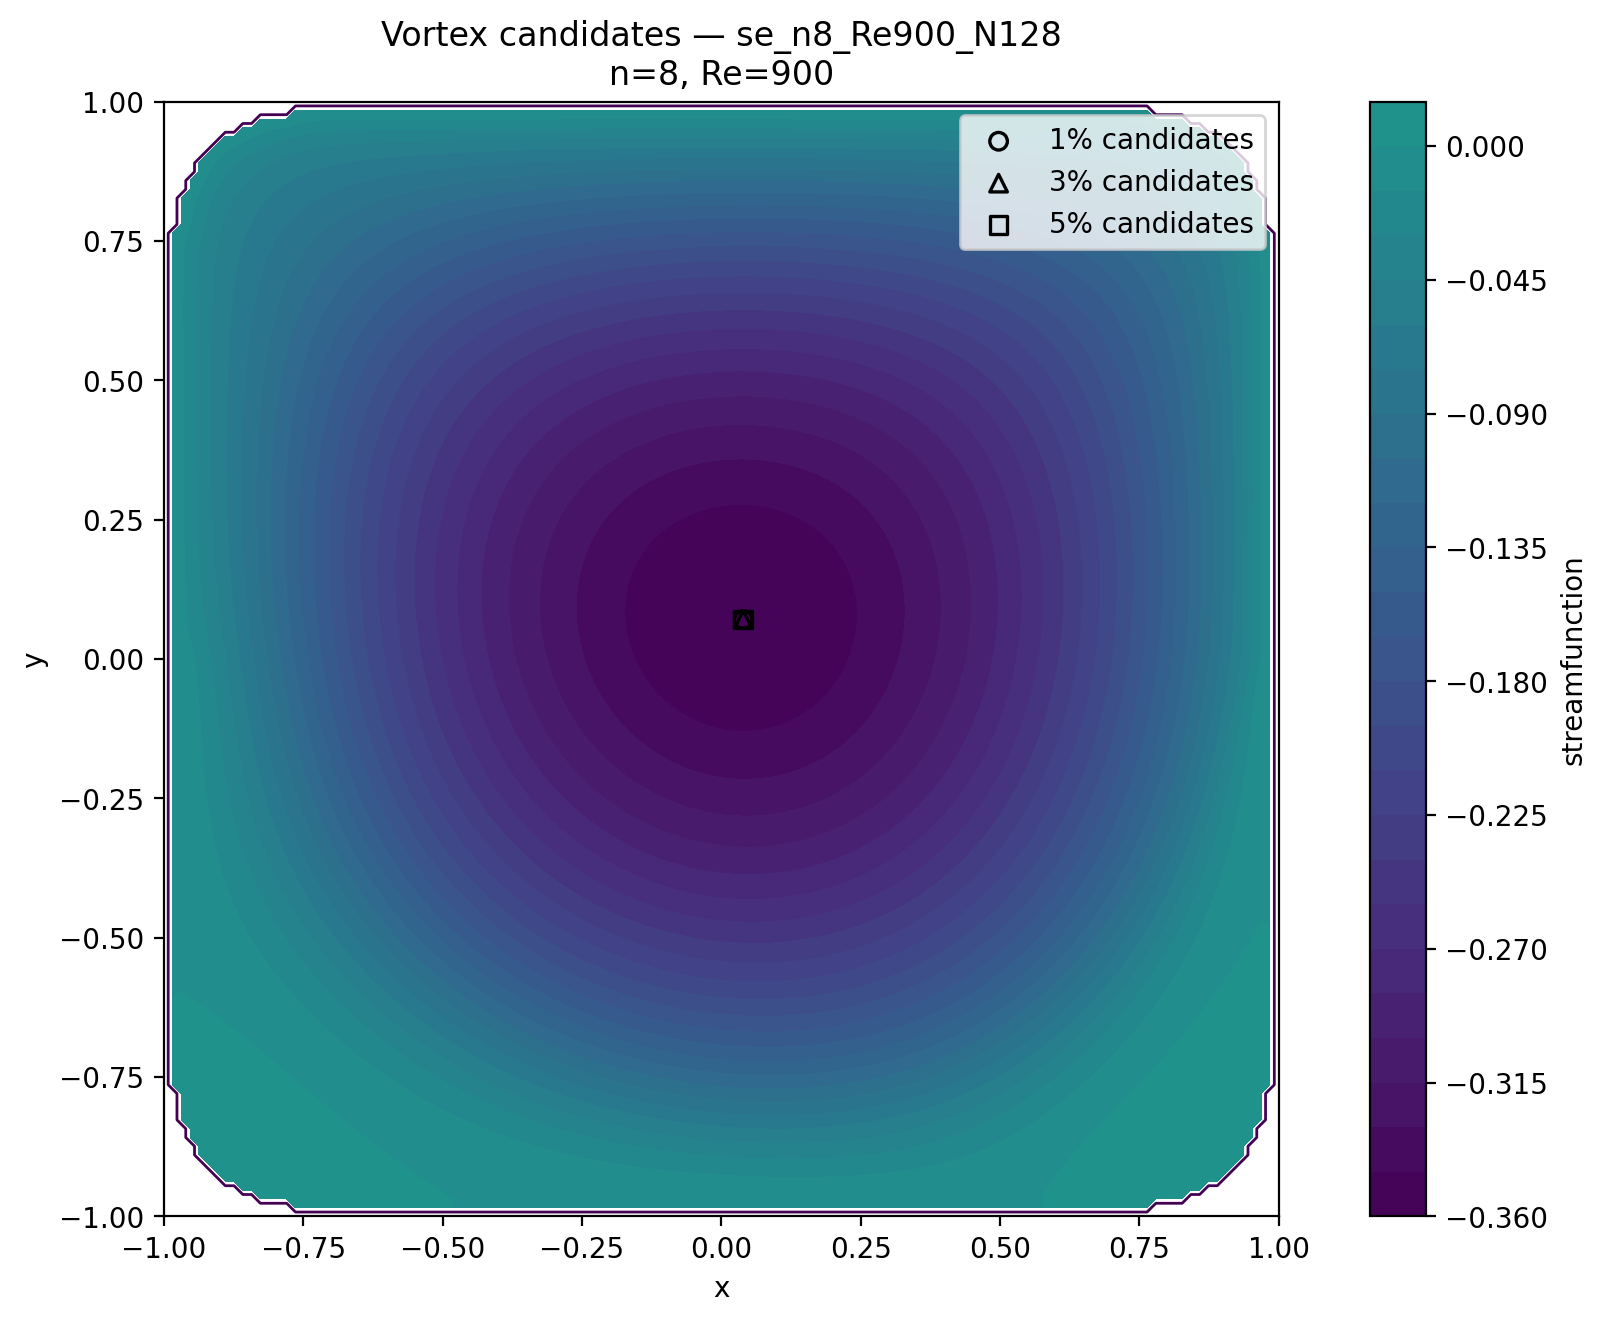
\includegraphics[width=\textwidth]{se_n8p0_Re900_N128_vortices.png} \caption{$n=8,\;Re=900$ --- one extremum} \end{subfigure} \hfill \begin{subfigure}[b]{0.31\textwidth} 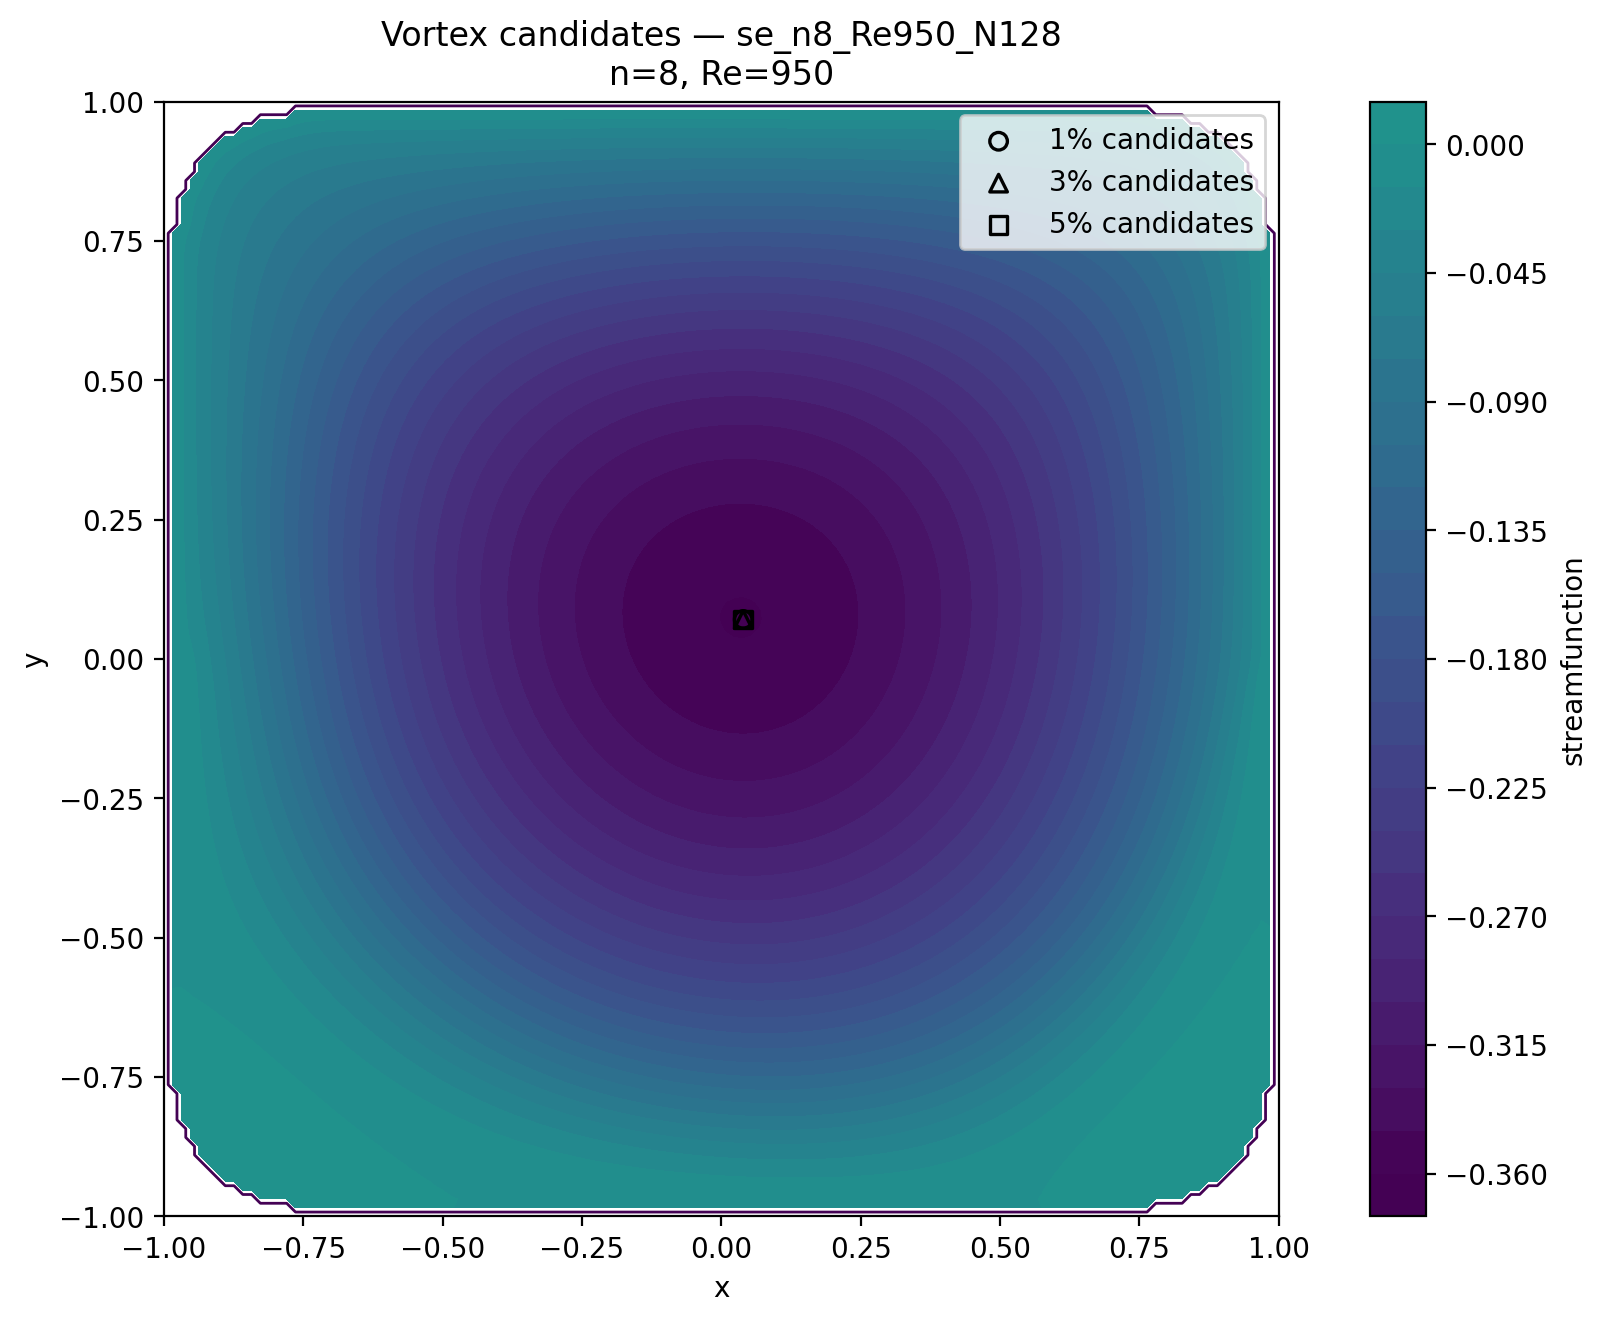
\includegraphics[width=\textwidth]{se_n8p0_Re950_N128_vortices.png} \caption{$n=8,\;Re=950$ --- one extremum} \end{subfigure} \hfill \begin{subfigure}[b]{0.31\textwidth} 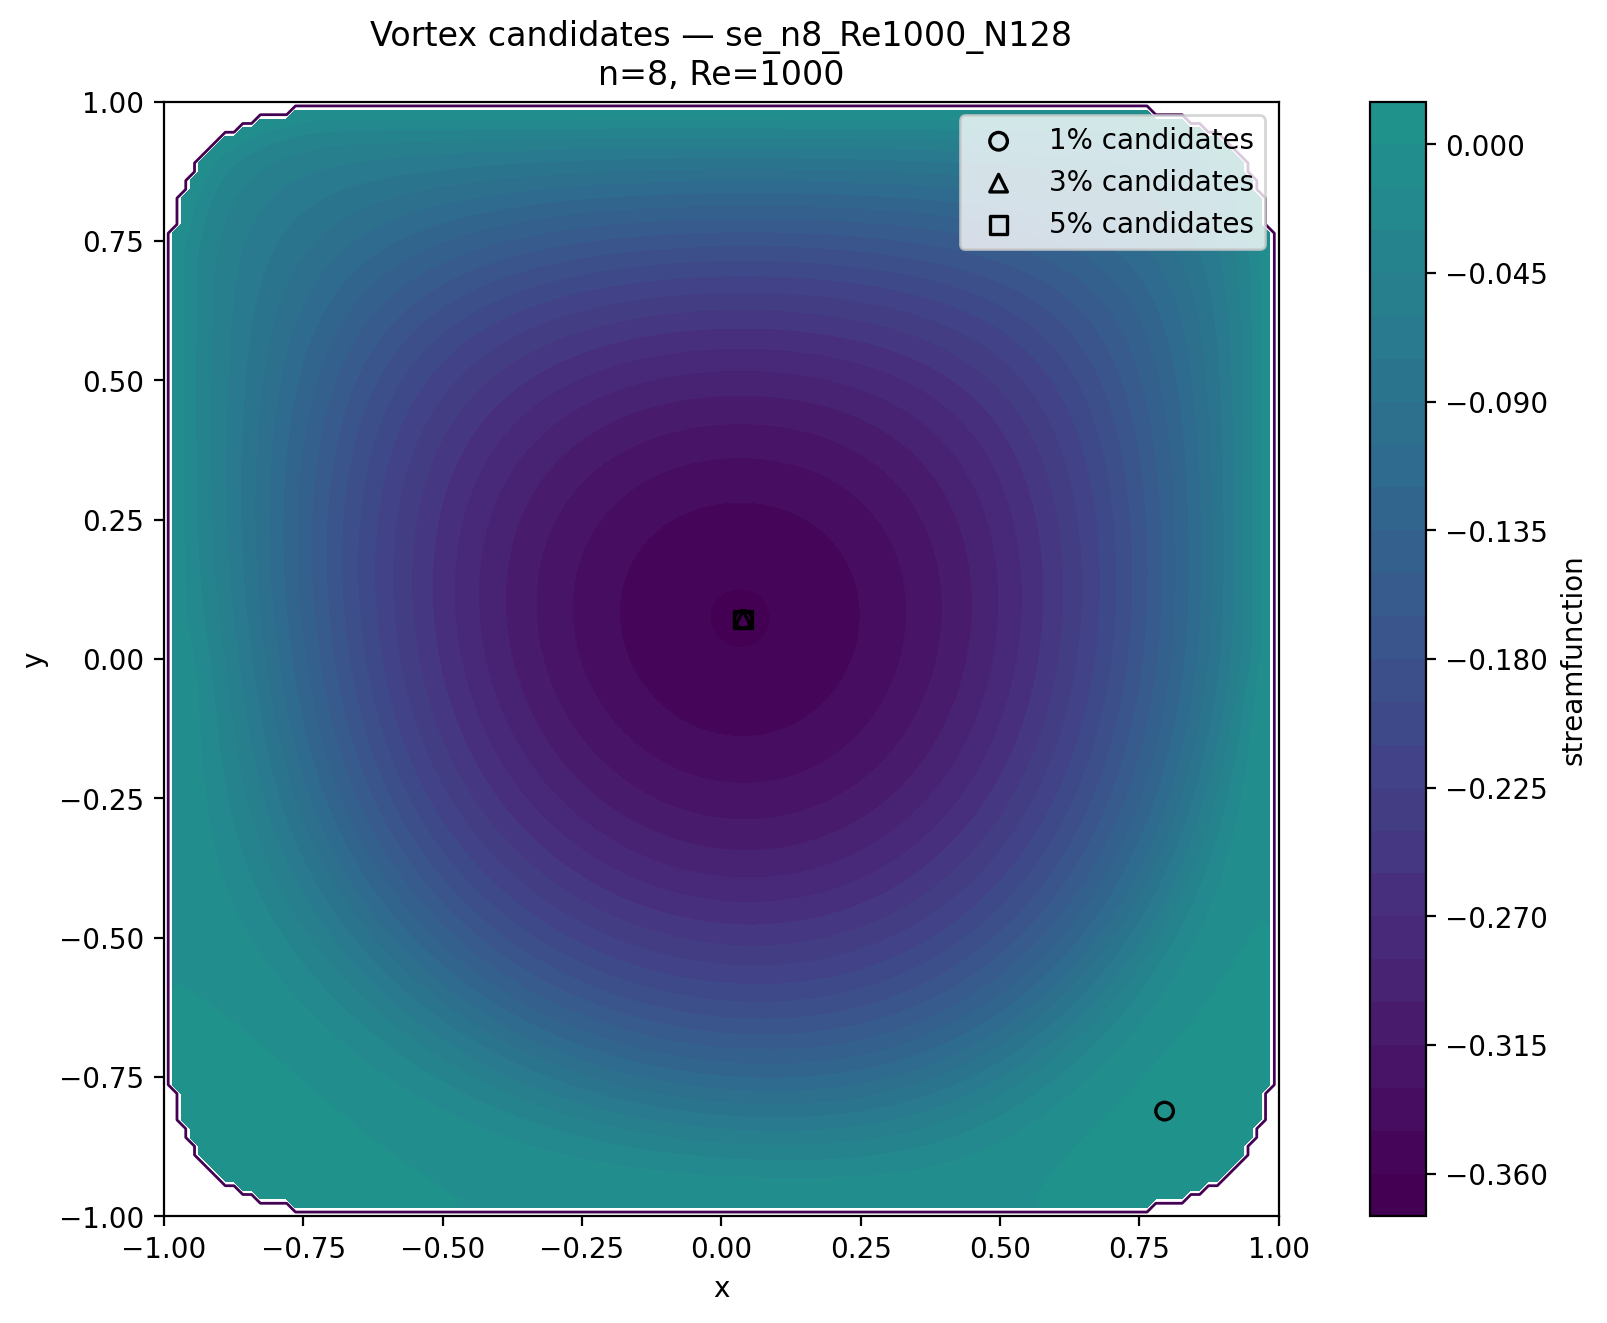
\includegraphics[width=\textwidth]{se_n8p0_Re1000_N128_vortices.png} \caption{$n=8,\;Re=1000$ --- two extrema} \end{subfigure}
\caption{Secondary corner extremum at $n=8$. Of the 190 cases on the grid, one
resolves a second extremum above the $1\%$ threshold of the primary circulation.
At $N=128$, the count changes from one to two between $Re=950$ and $Re=1000$;
this is a $1\%$ detection-threshold crossing bracket.}
\alttext{Secondary corner extremum at $n=8$. Of the 190 cases on the grid, one resolves a second extremum above the $1\%$ threshold of the primary circulation. At $N=128$, the count changes from one to two between $Re=950$ and $Re=1000$; this is a $1\%$ detection-threshold crossing bracket.}
\color{black}



\color{blue}
\label{fig:cornerbracket}
\color{black}
\end{figure}

\color{blue}
\section{Projected-lid boundary-law convention}\label{sec:lidlaw}
The reference forcing is the tangential law
$\mathbf{u}_{\rm lid}=U_{\rm lid}(m_y,-m_x)$ on the upper arc. For comparison
with conventional square-cavity implementations one may define a projected
tangential law by taking a horizontal translation $\mathbf{e}_x$ and projecting
it onto the local tangent,
$\mathbf{u}_{\rm lid}^{\rm proj}=U_{\rm lid}(\mathbf{e}_x\cdot\mathbf{t})\mathbf{t}$.
This is a kinematic definition only: the present study does not analyse
converged velocity fields generated with this alternative law, and no
hydrodynamic sensitivity is inferred from it. Its purpose is to make explicit
how the superelliptic family differs from the classical Ghia boundary
condition in the limit $n\to\infty$.

\section*{Data availability}
The post-processed data, analysis scripts, regenerated figures, result tables,
the final supplementary document and a description of the directory structure
are publicly available at
\url{https://github.com/Ahmedalgeria778/PH13_revision_data}. The repository
does not contain the manuscript source or the raw simulation fields. It is
distributed under the MIT License; see the \texttt{LICENSE} and \texttt{README.md}
files in the repository.

\color{black}

\bigskip
\section*{Appendix: material removed from the previous submission}
\noindent The following substantive lines were present in the previous submission (the 25 September 2026 supplementary submission) and are no longer part of the revised article. They are shown in red for traceability only; they are not part of the revised text.
\medskip
\color{red}
\begin{verbatim}
% =====================================================================
\large Supporting data, figures and additional insight for:\\
``Geometry-Induced Reorganization of Lid-Driven Flow in Continuously Deformable Superelliptic Cavities: Circulation, Dissipation, and Physics-Informed Operator Extrapolation beyond the Training Geometry Range''}
\noindent\textbf{Content of this document.} The Supplementary Material first
reports per-seed field accuracy and physical residuals, per-case comparison
metrics, the LBM finite-difference reference, and the individual field panels.
It then documents the complementary discussion, including the
seed-disagreement reliability diagnostic and the random-selection control
protocol, followed by the complete reference-solver verification chain and the
database quality control. The physical-observable definitions and the full
30-case energy and dissipation table are given next, together with the
complementary $Re=100$ reference field atlas and the per-placement metrics of
the $K=5$ random-selection control. The inference-only OOD distance map, the
126-case consistency--accuracy correlation audit, and the marginal cost curve
are reported in the same section. The final sections record the operator
implementation and training details moved out of the main text, the provenance
of the physical-regime synthesis, the curvature and near-wall dissipation
analysis of the locked fields, and the exploratory statistics together with the
residual maps relocated from the main text.
Figures and tables in this document are numbered S1, S2, ... and are not
duplicated in the main manuscript; the main text refers to them by number. The
sampled dissipation minima, the physical-regime synthesis figure, and the
per-case energy and dissipation table follow the same rule: each is presented
once, in the main manuscript, with the provenance recorded here.
\section{Per-seed field reconstruction accuracy}\label{sec:S1}
Table~\ref{tab:S1} reports the field coefficient of determination
$\Rtwo$ (mean over cases of each split) per seed for the three
physics-informed models.
\begin{table}[t]
\caption{Per-seed field $\Rtwo$ (mean over cases of each split) for the
physics-informed variants. ID denotes the in-distribution test split; OOD is report-only.}
\label{tab:S1}
\begin{tabular}{@{}lccccccc@{}}
\toprule
Model & Seed & Train & ID & OOD \\
\midrule
\multirow{3}{*}{B1-PI}
 & 40 & 0.99353 & 0.99170 & 0.97655 \\
 & 41 & 0.99334 & 0.99166 & 0.97430 \\
 & 42 & 0.99329 & 0.99179 & 0.97786 \\
\midrule
\multirow{3}{*}{B1-pinit}
 & 40 & 0.99410 & 0.99272 & 0.97482 \\
 & 41 & 0.99413 & 0.99283 & 0.97647 \\
 & 42 & 0.99414 & 0.99284 & 0.97818 \\
\midrule
\multirow{3}{*}{B1-train98}
 & 40 & 0.99330 & 0.99187 & 0.97625 \\
 & 41 & 0.99219 & 0.98988 & 0.97625 \\
 & 42 & 0.99238 & 0.99080 & 0.97374 \\
\bottomrule
\end{tabular}
\end{table}
\textbf{Insight.} The seed-to-seed spread of the OOD $\Rtwo$ is largest for
B1-PI (0.97430--0.97786) and smallest for B1-pinit (0.97482--0.97818);
B1-train98 lies in between (0.97374--0.97625). The three families
overlap on this metric within the seed dispersion, which supports the
``stability'' message of the main text: extending the physics-collocation
coverage from 77 to 98 cases does not degrade, nor does it improve, the OOD
field accuracy.
\section{Per-seed physical residuals}\label{sec:S2}
Table~\ref{tab:S2} collects the per-seed residual breakdown
($\Ldiv$, $\LNS$, $\Lp$) for every model and split; the boundary-condition
residual $\LBC$ is summarized in the text below to keep the table readable.
All residuals are
evaluated with the same 512-point collocation protocol used at training time.
\begin{table}[t]
\caption{Per-seed physical residuals on the train, ID and OOD splits.
$\Lp=(\mathrm{mean}\,p)^2$ is a pressure-head (DC) level, not a partial differential equation (PDE) residual;
it is reported descriptively.}
\label{tab:S2}
\resizebox{\textwidth}{!}{%
\begin{tabular}{@{}llccccccccc@{}}
\toprule
 &  & \multicolumn{3}{c}{Train} & \multicolumn{3}{c}{ID} & \multicolumn{3}{c}{OOD} \\
\cmidrule(lr){3-5}\cmidrule(lr){6-8}\cmidrule(lr){9-11}
Model & Seed & $\Ldiv$ & $\LNS$ & $\Lp$ & $\Ldiv$ & $\LNS$ & $\Lp$ & $\Ldiv$ & $\LNS$ & $\Lp$ \\
\midrule
\multirow{3}{*}{B1-PI}
 & 40 & 0.01519 & 0.23471 & 1.45e-4 & 0.01711 & 0.22602 & 1.60e-4 & 0.04957 & 0.27906 & 2.34e-4 \\
 & 41 & 0.01565 & 0.23142 & 3.52e-4 & 0.01767 & 0.22237 & 3.74e-4 & 0.04704 & 0.26544 & 4.65e-4 \\
 & 42 & 0.01581 & 0.23543 & 3.50e-5 & 0.01792 & 0.22832 & 4.20e-5 & 0.04954 & 0.28464 & 6.40e-5 \\
\midrule
\multirow{3}{*}{B1-pinit}
 & 40 & 0.01553 & 0.18528 & 4.20e-5 & 0.01754 & 0.18253 & 4.20e-5 & 0.05162 & 0.20327 & 4.30e-5 \\
 & 41 & 0.01581 & 0.18229 & 1.15e-4 & 0.01801 & 0.17990 & 1.16e-4 & 0.04855 & 0.18212 & 1.24e-4 \\
 & 42 & 0.01476 & 0.17606 & 3.50e-5 & 0.01663 & 0.17369 & 3.50e-5 & 0.05158 & 0.17629 & 5.50e-5 \\
\midrule
\multirow{3}{*}{B1-train98}
 & 40 & 0.00113 & 0.03469 & 3.12e-4 & 0.00121 & 0.03550 & 3.67e-4 & 0.00674 & 0.15060 & 4.10e-4 \\
 & 41 & 0.00128 & 0.03598 & 9.80e-4 & 0.00140 & 0.03734 & 1.09e-3 & 0.00491 & 0.12781 & 1.29e-3 \\
 & 42 & 0.00217 & 0.03582 & 5.39e-4 & 0.00233 & 0.03675 & 6.84e-4 & 0.00690 & 0.12376 & 1.13e-3 \\
\bottomrule
\end{tabular}%
}
\end{table}
The boundary-condition residual $\LBC$ (not tabulated per seed for
readability) ranges, in OOD, over $0.0216$--$0.0314$ for B1-PI,
$0.0306$--$0.0317$ for B1-pinit and $0.0208$--$0.0248$ for B1-train98.
\textbf{Insight.} B1-train98 is the only variant whose $\Ldiv$ sits below
$10^{-2}$ on every seed and every split, and whose train/ID $\LNS$ values are
all below $4\times10^{-2}$. The OOD $\LNS$ drop ($\approx0.28\to\approx0.13$)
and $\LBC$ drop are consistent across seeds, which strengthens the claim that
the 98-case physics-collocation extension improves the physical consistency of
the operator as a whole, not only the continuity residual.
\begin{figure}[t]
\includegraphics[width=\textwidth]{figS1_training_curves.png}
\caption{(a) B0 data mean-squared error (MSE; log scale, 1\,000 epochs). (b) B1-train98 composite
loss (log scale) for seeds 40, 41 and 42; the linear ramp reaches full physics
weight at epoch 300.}
\label{fig:S1}
\end{figure}
\begin{figure}[t]
\includegraphics[width=\textwidth]{figS2_seed_R2_ldiv.png}
\caption{Seed-wise OOD metrics. (a) OOD field $\Rtwo$ per seed.
(b) OOD divergence residual $\Ldiv$ per seed (log scale). The bars show the
three seeds 40, 41 and 42 for B1-PI, B1-pinit and B1-train98.}
\label{fig:S2}
\end{figure}
\section{Comparison configurations: per-case accuracy (seed 40)}\label{sec:S3}
Table~\ref{tab:S3} and Fig.~\ref{fig:S3} report the per-case seed-40 field
$\Rtwo$ of the four configurations shown in the comparison plate of the main
manuscript. Two configurations are ANCHOR cases ($n=2,Re=400$;
$n=3,Re=1000$): they belong to the physical-training pool of B1-train98 and
illustrate the local effect of the physics constraints extended to the anchor
instances. The other two are OOD cases
($n=5,Re=1000$; $n=8,Re=1000$) and illustrate geometry transfer. No ``ID''
label is used.
\begin{table}[t]
\caption{Per-case seed-40 field $\Rtwo$ of the comparison configurations
(seed 40).}
\label{tab:S3}
\begin{tabular}{@{}lccc@{}}
\toprule
Case & Type & B1-pinit & B1-train98 \\
\midrule
$n=2,\;Re=400$  & ANCHOR & 0.99662 & 0.99614 \\
$n=3,\;Re=1000$ & ANCHOR & 0.99049 & 0.98869 \\
$n=5,\;Re=1000$ & OOD    & 0.98464 & 0.98268 \\
$n=8,\;Re=1000$ & OOD    & 0.95008 & 0.95128 \\
\bottomrule
\end{tabular}
\end{table}
\begin{figure}[t]
\includegraphics[width=0.8\textwidth]{figS3_percase_R2.png}
\caption{Per-case seed-40 field $\Rtwo$ of the comparison configurations
(ANCHOR $n=2,Re=400$; ANCHOR $n=3,Re=1000$; OOD $n=5,Re=1000$;
OOD $n=8,Re=1000$), B1-pinit versus B1-train98.}
\label{fig:S3}
\end{figure}
\textbf{Insight.} On the two ANCHOR cases the B1-pinit model reaches the
highest $\Rtwo$ (0.9905--0.9966); B1-train98 is marginally below
($-5\times10^{-4}$ on $n=2$, $-1.8\times10^{-3}$ on $n=3$), consistent with
the additional physics terms reweighting the anchor data term in the composite
objective. On
the two OOD cases both models perform similarly ($\Delta\Rtwo$ of
$-2\times10^{-3}$ and $+1.2\times10^{-3}$), i.e. the extended physics
collocation neither degrades nor improves the OOD field reconstruction
case-by-case, in agreement with the aggregate result of the main manuscript.
\section{LBM finite-difference divergence reference}\label{sec:S4}
The physical LBM reference fields are almost divergence-free on the same
finite-difference grid used to define $\Ldiv$ in this study. Table~\ref{tab:S4}
and Fig.~\ref{fig:S4} give the per-split statistics. The comparison with the
neural-operator residuals is informational: the finite-difference operator and
its sampling are identical for both, but the LBM fields were not used to
constrain $\Ldiv$ during training.
\begin{table}[t]
\caption{Divergence residual of the LBM reference fields, evaluated with the
same finite-difference stencil as the training residual (per-split
min/mean/max over cases; LHS: Latin hypercube sampling).}
\label{tab:S4}
\begin{tabular}{@{}lcccc@{}}
\toprule
Split & $n$ & Min $\Ldiv$ & Mean $\Ldiv$ & Max $\Ldiv$ \\
\midrule
Train (77 LHS + 21 anchors) & 98 & $2.55\times10^{-4}$ & $3.89\times10^{-4}$ & $5.09\times10^{-4}$ \\
ID test (19 LHS)            & 19 & $2.62\times10^{-4}$ & $3.71\times10^{-4}$ & $5.02\times10^{-4}$ \\
OOD (9)                     &  9 & $1.26\times10^{-4}$ & $1.74\times10^{-4}$ & $2.09\times10^{-4}$ \\
\bottomrule
\end{tabular}
\end{table}
\begin{figure}[t]
\includegraphics[width=0.72\textwidth]{figS4_lbmfd_ref.png}
\caption{Mean LBM divergence residual by split, with min/max whiskers (log
scale).}
\label{fig:S4}
\end{figure}
\textbf{Insight.} The LBM reference satisfies $\Ldiv\lesssim5.1\times10^{-4}$
on all 126 cases. B1-train98 reaches $6.2\times10^{-3}$ (OOD), about 36 times
this reference level; the B1-pinit and B1-PI variants reach approximately
$5\times10^{-2}$, about 300 times the reference. The factor-of-36 observation
is reported descriptively: the neural operator residual and the reference are
evaluated with the same finite-difference stencil, but this does not constitute
a proof of PDE convergence.
\section{Training dynamics}\label{sec:S5}
Fig.~\ref{fig:S1} shows the training curves of the data-only B0 baseline
(1\,000 epochs) and of the three B1-train98 seeds (1\,500 epochs, AdamW,
learning rate $8\times10^{-4}$, weight decay $10^{-6}$, ramp over the first
300 epochs).
\textbf{Insight.} On all three seeds the recorded composite loss decreases over
the run, with the largest decrease occurring during the ramp phase and a
continued decay afterwards; no training instability is apparent in the recorded
curves. The improved physical consistency of B1-train98 is therefore observed
at the end of a stable training run rather than at an arbitrary early epoch;
the curves do not by themselves prove formal convergence of the optimization.
These results are reported descriptively.
\section{Seed-wise OOD dispersion}\label{sec:S6}
Fig.~\ref{fig:S2} summarizes the OOD field accuracy and OOD divergence
residual per seed for the three physics-informed models.
\textbf{Insight.} The OOD $\Ldiv$ of B1-pinit is $\approx5\times10^{-2}$ on
all three seeds, whereas the OOD $\Ldiv$ of B1-train98 is
$6.74\times10^{-3}$, $4.91\times10^{-3}$ and $6.90\times10^{-3}$, i.e.\ a
factor 8--10 lower on every seed. The multi-seed reproduction shows that the
$77\to98$ extension improves the OOD physical consistency robustly across the
three independent realizations; this statement is descriptive and does not, by
itself, establish a causal attribution to the anchor placement.
\section{Individual field panels}\label{sec:S7}
The four panels of the comparison plate in the main manuscript are
reproduced individually in Figs.~\ref{fig:S5}--\ref{fig:S8}. Each panel shows
the LBM reference, the B1-pinit velocity field, the B1-train98 velocity field
and the error fields (evaluation: seed 40). The velocity rows share the
per-case color scale anchored on
the LBM reference; the $|\mathbf{e}_u|$ row shares its scale across the two
models.
\begin{figure}[t]
\includegraphics[width=0.9\textwidth]{PH13_FigQ_anchor_n2_Re400.png}
\caption{ANCHOR case $n=2,\;Re=400$ (seed 40): LBM reference, B1-pinit,
B1-train98 and error fields.}
\label{fig:S5}
\end{figure}
\begin{figure}[t]
\includegraphics[width=0.9\textwidth]{PH13_FigQ_anchor_n3_Re1000.png}
\caption{ANCHOR case $n=3,\;Re=1000$ (seed 40): LBM reference, B1-pinit,
B1-train98 and error fields.}
\label{fig:S6}
\end{figure}
\begin{figure}[t]
\includegraphics[width=0.9\textwidth]{PH13_FigQ_ood_n5_Re1000.png}
\caption{OOD case $n=5,\;Re=1000$ (seed 40): LBM reference, B1-pinit,
B1-train98 and error fields.}
\label{fig:S7}
\end{figure}
\begin{figure}[t]
\includegraphics[width=0.9\textwidth]{PH13_FigQ_ood_n8_Re1000.png}
\caption{OOD case $n=8,\;Re=1000$ (seed 40): LBM reference, B1-pinit,
B1-train98 and error fields.}
\label{fig:S8}
\end{figure}
\section{Complementary discussion}\label{sec:S8}
\subsection{Decoupling between field accuracy and physical consistency}
The OOD field $\Rtwo$ varies by less than $1.1\times10^{-3}$ across the
physics-informed family while the OOD divergence residual spans approximately
one order of magnitude, from $5.06\times10^{-2}$ (B1-pinit)
to $6.18\times10^{-3}$ (B1-train98). The comparison of B0
(data-only) with B1-pinit and B1-train98 shows that a well-reconstructed
velocity field is not a certificate of a small PDE residual: B0 reaches
$\Rtwo\approx0.989$ (train) while its $\Ldiv$ is
$1.5\times10^{-2}$--$2.8\times10^{-2}$. The two evaluation levels are
complementary and both are reported in this study.
\subsection{\texorpdfstring{The pressure-head indicator $\Lp$}{The pressure-head indicator Lp}}
$\Lp=(\mathrm{mean}\,p)^2$ measures only the DC level of the pressure head;
it is neither a PDE residual nor a measure of pressure-field quality. The
B1-pinit variant drives $\Lp$ to $\approx5\times10^{-5}$--$10^{-4}$ on all
splits, because its pressure output is not trained and stays pinned near the
initialization. B1-train98 re-engages the pressure head
($\sim10^{-3}$--$10^{-4}$) alongside its reduced OOD momentum residual
(~2$\times$ drop of the OOD
$\LNS$, Table~\ref{tab:S2}). $\Lp$ is a gauge (DC) level: it does not measure
the accuracy of the pressure-gradient field, so this co-variation is reported
descriptively and no claim is made about the reconstructed pressure field.
\subsection{Kinetic-energy and maximum-velocity relative errors}
The OOD kinetic-energy relative error (ke\_rel\_err) of B1-train98 spreads
over $0.022$, $0.054$ and $0.060$ across the seeds -- wider than its field
$\Rtwo$ spread. This metric is sensitive to the small-velocity regions and is
reported as-is, without correction or post-selection. The OOD
maximum-velocity relative error (umax\_rel\_err) of B1-train98 is more
stable, $0.0259$, $0.0271$ and $0.0290$. These secondary metrics do not
affect any finding of the main manuscript.
\subsection{Normalization constants of the physics losses}
The reference magnitudes used to normalize each physics term before
weighting (fixed mini-batch of LHS cases at initial weights, seed-40 probe)
are $L^0_{\mathrm{data}}\approx1.655\times10^{-3}$,
$L^0_{\mathrm{div}}\approx4.341\times10^{-3}$,
$L^0_{\mathrm{NS}}\approx2.466\times10^{-1}$ and
$L^0_{\mathrm{BC}}\approx5.097\times10^{-2}$. The pressure-head reference is
$L^0_p=1.0$, the unit DC level of the pinit initialization (pressure-branch
bias zeroed and scalar pressure addend set to one before PI training). The loss weights used throughout the PI family are
$\lambda_{\mathrm{div}}=1$, $\lambda_{\mathrm{NS}}=1$,
$\lambda_{\mathrm{BC}}=1$ and $\lambda_p=0.25$, with a linear ramp over the
first 300 epochs.
\subsection{Random-selection control for the
\texorpdfstring{$77\to98$}{77 to 98} extension}
The main manuscript reports that extending the physics constraints from the 77
LHS configurations to the 98-case pool (B1-pinit $\to$ B1-train98) improves the
OOD physical consistency by approximately one order of magnitude on $\Ldiv$,
and it states that this gain cannot be attributed to additional supervised
data: as established above, the anchors already contribute their
velocity fields to \emph{all} operators, so the supervised data pool (77 LHS +
21 anchors) is identical in B1-pinit and B1-train98; the only variation is the
coverage of the physics collocation points (77 vs.\ 98). What this comparison
cannot yet separate is whether the gain comes from the \emph{number} of
physics-constrained instances or from the \emph{deterministic placement} of the
added anchors. This subsection describes the control experiment designed to
separate the two and reports its outcome. The OOD cases remain report-only.
\paragraph{Design.} Three groups share the fixed architecture, hyperparameters
($\lambda_{\mathrm{div}}=\lambda_{\mathrm{NS}}=\lambda_{\mathrm{BC}}=1$,
$\lambda_p=0.25$, ramp 300 epochs) and OOD evaluation protocol:
\begin{itemize}
  \item \textbf{A} -- 77 LHS physics-constrained cases only (the B1-pinit
        configuration);
  \item \textbf{B} -- 98 cases consisting of the 77 LHS cases plus $21$
        parameter instances drawn uniformly in $n$ and uniformly in
        $\log_{10}Re$ over the LHS parameter domain ($n\in[1.26,3.98]$,
        $Re\in[101.1,977.3]$, taken from the min/max of the 96 stored LHS
        configurations), sampled without replacement and excluding the $21$
        deterministic anchors. The five placements use sampling seeds
        20260922--20260926; the first reuses the seed-40 member of the locked
        checkpoint without retraining, and the four additional placements use
        internal seed 40;
  \item \textbf{C} -- 98 cases consisting of the 77 LHS cases plus the $21$
        deterministic anchors (the B1-train98 configuration).
\end{itemize}
Thus groups B and C add the same number of physics-constrained instances
($N_{\mathrm{physics}}=98$); the $21$ random instances are physics-only
collocation locations, carrying no LBM reference field and contributing no
supervised velocity target. Groups A and C retain the three internal seeds
40, 41 and 42 for their locked diagnostics, while the K=5 group-B estimate
averages the five placement means. All configurations share the identical
98-case supervised data pool, so any difference across A, B and C isolates
the physics-collocation contribution. The legacy locked group-B diagnostic
for placement 20260922, averaged over internal seeds 40, 41 and 42, is kept
as $\Ldiv=3.56\times10^{-3}$ for traceability; it is not the K=5 estimate.
\paragraph{Decision rule.} The groups are compared on the OOD metrics of the
main manuscript, $\Ldiv$, $\LNS$, $\LBC$ and $\Rtwo$. Let $B$ denote the set
of the $K=5$ random placements:
\begin{itemize}
  \item if $C\approx B > A$ on the residual metrics at comparable $\Rtwo$, the
        result supports a primary role for increased coverage of
        physics-constrained instances, with anchor placement not isolated as the
        deciding factor;
  \item if $C < B$ on $\Ldiv$ (and consistently on $\LNS$, $\LBC$) at
        comparable $\Rtwo$, the \emph{deterministic anchor placement} would support
        an additional physical benefit beyond coverage.
\end{itemize}
\paragraph{Outcome ($K=5$).} The OOD residuals of group B, reported as
mean~$\pm$~standard deviation over the five placements, are
$\Ldiv=4.39\times10^{-3}\pm1.52\times10^{-3}$,
$\LNS=6.71\times10^{-2}\pm9.83\times10^{-3}$ and
$\LBC=3.40\times10^{-2}\pm5.27\times10^{-3}$, compared with
$\Ldiv=6.18\times10^{-3}$, $\LNS=1.34\times10^{-1}$ and
$\LBC=2.34\times10^{-2}$ for group C (anchors), and
$\Ldiv=5.06\times10^{-2}$, $\LNS=1.87\times10^{-1}$ and
$\LBC=3.11\times10^{-2}$ for group A (77 LHS only). The K=5 group therefore
reaches \emph{lower} $\Ldiv$ and $\LNS$ than the deterministic anchors, but a
larger $\LBC$, and it attains the residual reduction at a lower field accuracy
($\Rtwo=0.9661\pm0.0044$ versus $0.9754\pm0.0015$ for group C). Under the
decision rule, the $77\to98$ residual reduction is reproduced by randomly placed
instances, which is consistent with an important role for the \emph{number} and
coverage of physics-constrained instances; the comparison does not isolate
deterministic placement as the sole mechanism. The anchor grid offers the
more balanced accuracy--boundary-condition trade-off in this comparison. The
K=5 spread is placement variability, not a formal model-selection
uncertainty. Table~\ref{tab:S11} reports all five placements.
\subsection{Seed-disagreement reliability diagnostic}
The three internal-seed realizations of the locked physics-informed families
also provide a minimal ensemble for an exploratory reliability diagnostic. On each
OOD configuration, the per-point inter-seed standard deviation $\delta$ of
the predicted velocity field is compared with the per-point reconstruction
error relative to the LBM reference. Pooled over the nine OOD configurations
(138{,}816 fluid nodes), the Spearman correlation is $\rho=0.355$ (Pearson
correlation on log-transformed quantities: $r=0.339$); per configuration,
$\rho\in[0.157,0.518]$, with the largest values ($\rho\approx0.5$) attained on
the near-square $n=6$--$8$ geometries at intermediate and high Reynolds
number. Seed disagreement is therefore positively associated with prediction
error in the present exploratory analysis --- nodes on which the three
realizations disagree are associated with larger errors --- but
the three-seed ensemble is insufficient for calibrated uncertainty estimation
or coverage claims. The diagnostic is reported descriptively and is not used
for model selection.
\section{Reference solver verification}\label{sec:S9}
the complete verification chain of that solver: (i) the square-cavity baseline against the classic data
of Ghia et al.\ (1982) and the associated grid convergence index (GCI) control
(Table~\ref{tab:S5}, Figs.~\ref{fig:S9}--\ref{fig:S10}); (ii) the
curved-boundary test against the exact rigid-rotation solution
(Table~\ref{tab:S6}); and (iii) the cross-validation of representative LBM
fields against an independent FEM formulation
(Table~\ref{tab:S7}, Figs.~\ref{fig:S11}--\ref{fig:S13}).
$U_{\mathrm{ref}}=0.05$ and characteristic length $L_{\mathrm{char}}=127$
lattice units, i.e.\ the diameter of the discrete $N=128$ cavity (2 in the
continuous units of the main manuscript). The continuous normalization of the
$x_{\mathrm{lbm}}=x\,L_{\mathrm{char}}$ relate the two reference systems and
give the same physical Reynolds number. The curved superelliptic
$\mathbf{u}_{\mathrm{lid}}=U_{\mathrm{lid}}(n_y,-n_x)$ on the interpolated
boundary nodes. Steady state is declared when the maximum change of the
macroscopic velocity over a sliding window of 100 iterations satisfies
$\mathrm{d}u_{\max}<10^{-8}$, with the check active only after at least 500
iterations; for the production superelliptic cases the run stops at a hard
maximum of 200{,}000 iterations, while the square-cavity baseline uses a
separate larger budget (e.g.\ 794{,}000 iterations at $Re=1000$,
Table~\ref{tab:S5}). The maximal density-level residual is below $10^{-8}$.
comparison. All FEM solves reported in Table~\ref{tab:S7} converged to the
\subsection{Square-cavity baseline and grid convergence}
Table~\ref{tab:S5} reports the $L_2$ and $L_\infty$ discrepancies of the
center-line velocity profiles against the Ghia et al.\ reference on the
uniform-lid square cavity at $N=256$, together with the number of iterations
and the final residual norm of the MRT solver. Fig.~\ref{fig:S9} shows the
center-line profiles overlaid on Ghia et al.  for $Re=100$ and $Re=1000$;
Fig.~\ref{fig:S10} summarizes the grid-convergence (GCI) study carried out at
$Re=500$ with the controlled two-harmonic lid profile ($A_2\sin(2\pi x)$),
from which the observed order and the discretization error estimate are taken.
These GCI quantities qualify the square-cavity baseline solver; their transfer
to the curved-boundary production cases is asserted as an indicative
consistency check rather than as a strict guarantee.
\begin{table}[t]
\label{tab:S5}
1000  & $1.41\times10^{-2}$ & $3.00\times10^{-2}$ & $1.32\times10^{-2}$ &
$2.12\times10^{-2}$ & 794\,000 & $9.64\times10^{-10}$ \\
\begin{figure}[t]
Table~\ref{tab:S5}.}
\label{fig:S9}
\begin{figure}[t]
\includegraphics[width=\textwidth]{figS10_grid_convergence.png}
\caption{Grid-convergence (GCI) study of the square-cavity solver at
$Re=500$ with the controlled two-harmonic lid profile: resolved integral norm
$\epsilon$ versus $N\in\{128,256,512\}$, Richardson-extrapolated value
$\epsilon^*$, observed order $p$ and grid-convergence index.}
\label{fig:S10}
\end{figure}
Table~\ref{tab:S6} reports, for $N\in\{32,48,64,96\}$, the $L_2$ and $L_\infty$
errors of the numerical field, the maximum wall-normal leakage
$\max|u\cdot n|$ on the curved boundary, the iteration count and the final
residual. The wall-normal leakage is the decisive metric for the
interpolated-bounce-back treatment (Bouzidi scheme): it decreases from
$4.41\times10^{-5}$ at $N=32$ to $2.06\times10^{-5}$ at $N=96$, i.e.\ the
wall-normal leakage decreases with resolution, consistent with a reduction
of discretization error ($Re=100$).
\begin{table}[t]
$u=(y,-x)$ of a rotating disk ($Re=100$): $L_2$/$L_\infty$ errors, maximum
wall-normal leakage $\max|u\cdot n|$, iterations and final residual.}
\label{tab:S6}
$N$ & $L_2$ & $L_\infty$ & $\max|u\cdot n|$ & Iterations & Residual \\
32 & $9.35\times10^{-4}$ & $1.29\times10^{-3}$ & $4.41\times10^{-5}$ & 18\,000 & $9.18\times10^{-11}$ \\
48 & $9.85\times10^{-4}$ & $1.34\times10^{-3}$ & $3.35\times10^{-5}$ & 26\,800 & $9.77\times10^{-11}$ \\
64 & $1.01\times10^{-3}$ & $1.38\times10^{-3}$ & $2.18\times10^{-5}$ & 35\,500 & $9.61\times10^{-11}$ \\
96 & $1.04\times10^{-3}$ & $1.41\times10^{-3}$ & $2.06\times10^{-5}$ & 52\,400 & $9.84\times10^{-11}$ \\
\label{sec:S9c}
To validate the MRT-LBM solver across the geometric family, an independent cross-validation is performed against a finite-element method (FEM) solver using Taylor--Hood $\mathbb{P}_2/\mathbb{P}_1$ elements with Picard iteration. Four representative cavity geometries are considered: circle ($n=2$), ellipse ($n=1.5$), super-ellipse ($n=4$), and square ($n\to\infty$). Table~\ref{tab:S7} reports the interior relative $L_2$ discrepancy between LBM and FEM at $Re\in\{100,400\}$. All discrepancies are below $1.5\,\%$, with a mild increase at $Re=400$ due to the thinner boundary layers. Figs.~\ref{fig:S11} and~\ref{fig:S12} show the velocity field overlays at $Re=100$ and $Re=400$ respectively; the corresponding interior relative $L_2$ discrepancies are reported in Table~\ref{tab:S7}.
The grid-convergence study (Fig.~\ref{fig:S13}) on the circle geometry at $Re=100$ shows that the interior $L_2$ discrepancy decreases from $1.48\times10^{-2}$ at $N=32$ to $2.20\times10^{-3}$ at $N=96$, tracking between the $O(h)$ and $O(h^2)$ references. The observed decrease is consistent with a reduction of discretization error over the tested resolutions; the order is reported descriptively and no explicit convergence-rate claim is made beyond this $O(h)$--$O(h^2)$ range. At the production resolution range considered here ($N=96$--$128$), the remaining LBM--FEM discrepancy is consistent with a finite-resolution contribution; the available grids do not justify a stronger asymptotic statement. These results are reported descriptively and do not affect any finding of the main manuscript.
\begin{table}[t]
independent FEM solution for four cavity geometries at $Re\in\{100,400\}$.
$N=64$ (FEM $n_{\mathrm{refs}}=5$) at $Re=100$; $N=96$ (FEM $n_{\mathrm{refs}}=6$)
at $Re=400$. All LBM residuals below $10^{-8}$; all FEM solves converged.}
\label{tab:S7}
\begin{tabular}{@{}lcc@{}}
Geometry ($n$) & $Re=100$ & $Re=400$ \\
Circle ($n=2$)        & 0.93 & 1.20 \\
Ellipse ($n=1.5$)     & 1.06 & 1.20 \\
Super-ellipse ($n=4$) & 0.96 & 1.45 \\
Square ($n\to\infty$) & 0.87 & 1.21 \\
\end{tabular}
\begin{figure}[htbp]
($N=64$, FEM $n_{\mathrm{refs}}=5$). Each panel overlays the LBM and FEM
$L_2$ discrepancies are reported in Table~\ref{tab:S7}.}
\label{fig:S11}
\begin{figure}[htbp]
($N=96$, FEM $n_{\mathrm{refs}}=6$). The comparison remains within the reported
below $1.5\,\%$ (Table~\ref{tab:S7}).}
\label{fig:S12}
\begin{figure}[htbp]
\label{fig:S13}
\section{Database quality control}\label{sec:S10}
the $30$-case physics-analysis subset (all $10$ exponents $n$ at
$Re\in\{100,400,1000\}$, $N=128$). Table~\ref{tab:S8} condenses the quality-control
report: $30$ cases found
domain $0.95\,\%$ (below the $1\,\%$ acceptance threshold), maximum LBM residual
$9.999\times10^{-9}$ (below $10^{-8}$), and positive minimum density.
$u_w=U_{\mathrm{lid}}(n_y,-n_x)$ is not invariant under reflection
(\emph{not applicable} status). Pressure is not present
in the production NumPy archive (NPZ) files; drag, wall traction and exact lid mechanical
power are therefore never inferred. Fig.~\ref{fig:S14} shows the spatial
(Table~\ref{tab:S8}), is attained at a single isolated interior cell of the most
\begin{table}[t]
\caption{Database quality-control summary ($30$ cases analysed,
$N=128$).}
\label{tab:S8}
Cases found / analysed & 30 / 30 & --- \\
Max.\ relative area error & $9.5\times10^{-3}$ & pass ($<10^{-2}$) \\
Max.\ LBM residual & $9.999\times10^{-9}$ & pass ($<10^{-8}$) \\
Pressure available & no & not inferred \\
\begin{figure}[t]
\label{fig:S14}
\section{Physical observables of the comparison configurations}\label{sec:S11}
for $q\in\{1,3,5\}\,\%$. The area-normalized observables of
Table~\ref{tab:S10} are obtained by dividing the integrated quantities by the
exact cavity area $A(n)=4\,\Gamma(1+1/n)^2/\Gamma(1+2/n)$ for $a=b=1$
(the area formula in the main manuscript).
Table~\ref{tab:S9} provides the numerical values of the physical observables
associated with the four configurations used in the qualitative comparison of
the main manuscript: two ANCHOR cases and two OOD cases. These values are
provided to facilitate quantitative inspection of the representative fields
and to document the flow characteristics independently of the neural-operator
metrics discussed in the main text. The table includes maximum velocity,
\begin{table}[t]
\label{tab:S9}
\resizebox{\textwidth}{!}{%
ANCHOR $n=2,Re=400$    & 0.998 & 21.4  & $-0.337$ & 1 / 1 & 0.0467 & 0.357 & 7.69 & 0.0334 \\
ANCHOR $n=3,Re=1000$   & 1.039 & 24.6  & $-0.360$ & 1 / 1 & 0.0248 & 0.409 & 9.02 & 0.0408 \\
OOD $n=5,Re=1000$      & 1.035 & 24.6  & $-0.363$ & 1 / 1 & 0.0265 & 0.422 & 9.33 & 0.0395 \\
OOD $n=8,Re=1000$      & 1.027 & 24.5  & $-0.361$ & 2 / 1 & 0.0284 & 0.421 & 9.67 & 0.0391 \\
Table~\ref{tab:S10} is the per-case source of the energy and dissipation
analysis of the main manuscript. The interpretation of those columns --- the
provenance of the synthesis is documented in Sec.~S14 and the additional
curvature and near-wall analysis in Sec.~S15.
\begin{table}[t]
\caption{Exact cavity area $A(n)$, integrated kinetic energy $KE$, integrated
dissipation $D$ and their area-normalized counterparts $KE/A$ and $D/A$ for
the 30-case physics-analysis grid ($N=128$). Dissipation follows the standard
mechanical definition $D=2\nu\int_{\Omega}S:S\,dA$ with $\nu=2/Re$
(Sec.~S11).}
\label{tab:S10}
\small
\begin{tabular}{@{}rrrrrrr@{}}
$n$ & $Re$ & $A(n)$ & $KE$ & $KE/A$ & $D$ & $D/A$ \\
 1.25 &   100 &   2.4271 &   0.2221 &   0.0915 &   0.1873 &   0.07716 \\
   1.5 &   100 &   2.7379 &   0.2722 &   0.0994 &   0.1423 &   0.05197 \\
  1.75 &   100 &   2.9678 &   0.3083 &   0.1039 &   0.1245 &   0.04194 \\
     2 &   100 &   3.1416 &   0.3313 &   0.1055 &   0.1162 &   0.03700 \\
   2.5 &   100 &   3.3809 &   0.3572 &   0.1057 &   0.1122 &   0.03318 \\
     3 &   100 &   3.5333 &   0.3669 &   0.1038 &   0.1141 &   0.03228 \\
     4 &   100 &   3.7081 &   0.3729 &   0.1006 &   0.1222 &   0.03296 \\
     5 &   100 &   3.8006 &   0.3729 &   0.0981 &   0.1309 &   0.03444 \\
     6 &   100 &   3.8552 &   0.3709 &   0.0962 &   0.1388 &   0.03600 \\
     8 &   100 &   3.9138 &   0.3671 &   0.0938 &   0.1522 &   0.03890 \\
 1.25 &   400 &   2.4271 &   0.2388 &   0.0984 &   0.0643 &   0.02650 \\
   1.5 &   400 &   2.7379 &   0.2933 &   0.1071 &   0.0536 &   0.01957 \\
  1.75 &   400 &   2.9678 &   0.3320 &   0.1119 &   0.0491 &   0.01655 \\
     2 &   400 &   3.1416 &   0.3567 &   0.1135 &   0.0467 &   0.01488 \\
   2.5 &   400 &   3.3809 &   0.3838 &   0.1135 &   0.0455 &   0.01347 \\
     3 &   400 &   3.5333 &   0.3941 &   0.1115 &   0.0458 &   0.01297 \\
     4 &   400 &   3.7081 &   0.4019 &   0.1084 &   0.0479 &   0.01291 \\
     5 &   400 &   3.8006 &   0.4037 &   0.1062 &   0.0501 &   0.01317 \\
     6 &   400 &   3.8552 &   0.4032 &   0.1046 &   0.0520 &   0.01348 \\
     8 &   400 &   3.9138 &   0.4018 &   0.1027 &   0.0551 &   0.01408 \\
 1.25 &  1000 &   2.4271 &   0.2461 &   0.1014 &   0.0329 &   0.01357 \\
   1.5 &  1000 &   2.7379 &   0.3041 &   0.1111 &   0.0285 &   0.01041 \\
  1.75 &  1000 &   2.9678 &   0.3454 &   0.1164 &   0.0266 &   0.00896 \\
     2 &  1000 &   3.1416 &   0.3713 &   0.1182 &   0.0255 &   0.00810 \\
   2.5 &  1000 &   3.3809 &   0.3986 &   0.1179 &   0.0248 &   0.00735 \\
     3 &  1000 &   3.5333 &   0.4090 &   0.1158 &   0.0248 &   0.00702 \\
     4 &  1000 &   3.7081 &   0.4186 &   0.1129 &   0.0256 &   0.00690 \\
     5 &  1000 &   3.8006 &   0.4216 &   0.1109 &   0.0265 &   0.00697 \\
     6 &  1000 &   3.8552 &   0.4211 &   0.1092 &   0.0272 &   0.00706 \\
     8 &  1000 &   3.9138 &   0.4208 &   0.1075 &   0.0284 &   0.00725 \\
\section{Reference flow field atlas}\label{sec:S12}
This section complements the main-text reference-flow atlas by providing the reference LBM flow fields at the lower Reynolds number $Re=100$. Figure~\ref{fig:S15} shows the velocity magnitude and streamfunction, illustrating the steady characteristics for representative geometries. The corresponding fields and vortex topologies at $Re=1000$ are discussed in the main text.
\begin{figure}[htbp]
\label{fig:S15}
\begin{table}[htbp]
\caption{Per-placement OOD metrics of the matched-count random-selection
control (group B, $K=5$): field accuracy $\Rtwo$ and physical residuals
($\Ldiv$, $\LNS$, $\LBC$) on the nine OOD configurations. Each additional
placement uses internal seed 40; placement 20260922 reuses its locked seed-40
member without retraining. The mean and standard deviation are over placements,
not internal seeds. The legacy three-seed diagnostic for 20260922 is retained in
the text separately.}
\label{tab:S11}
\resizebox{\textwidth}{!}{%
\begin{tabular}{@{}lcccc@{}}
Placement & ${\Rtwo}_{\mathrm{OOD}}$ & ${\Ldiv}_{\mathrm{OOD}}$ &
${\LNS}_{\mathrm{OOD}}$ & ${\LBC}_{\mathrm{OOD}}$ \\
20260922 & 0.96302 & $3.79\times10^{-3}$ & $6.59\times10^{-2}$ & $3.78\times10^{-2}$ \\
20260923 & 0.97388 & $2.86\times10^{-3}$ & $5.14\times10^{-2}$ & $3.35\times10^{-2}$ \\
20260924 & 0.96348 & $6.86\times10^{-3}$ & $6.95\times10^{-2}$ & $2.51\times10^{-2}$ \\
20260925 & 0.96492 & $4.70\times10^{-3}$ & $7.81\times10^{-2}$ & $3.72\times10^{-2}$ \\
20260926 & 0.96526 & $3.76\times10^{-3}$ & $7.05\times10^{-2}$ & $3.66\times10^{-2}$ \\
Mean $\pm$ SD & $0.96611\pm0.00444$ & $4.39\times10^{-3}\pm1.52\times10^{-3}$ &
$6.71\times10^{-2}\pm9.83\times10^{-3}$ & $3.40\times10^{-2}\pm5.27\times10^{-3}$ \\
\end{tabular}%
}
\subsection{Inference-only OOD distance and geometry-induced extrapolation}
\label{sec:supp:oodmap}
The frozen checkpoints were evaluated without additional training or new
LBM simulations on a deterministic $N=128$ superellipse grid. The geometry
sweep uses $n\in\{4.5,5,6,8,10,12,16\}$ and
$Re\in\{100,400,1000\}$; the geometry--Reynolds-number matrix uses
$(n,Re)\in\{2,5,8\}\times\{1200,1500,2000\}$. The residual-only geometry is
$|x|^n+|y|^n<1$, and the sampling seed for each point is derived from its
canonical case identifier. A normalized parameter-space distance is measured from the
frozen training box $n\in[1.25,4]$, $\log_{10}Re\in[2,3]$, with each
coordinate normalized by its box width. The nine points with
$n\in\{5,6,8\}$ and $Re\in\{100,400,1000\}$ are the existing LBM reference
cases; the other points support residual and distance diagnostics only.
\begin{table}[htbp]
\caption{Selected $\Ldiv$ values from the inference-only OOD map. The
reference flag is restricted to the nine existing LBM cases; no field accuracy
is inferred for synthetic points.}
\label{tab:oodmap_supp}
\resizebox{\textwidth}{!}{%
\begin{tabular}{@{}lrrrr@{}}
$(n,Re)$ & B0 & B1-pinit & B1-train98 & B1-rand98 \\
$(4.5,1000)$ & $1.950{\times}10^{-2}$ & $1.658{\times}10^{-2}$ & $2.645{\times}10^{-3}$ & $1.469{\times}10^{-3}$ \\
$(5,1000)$   & $2.536{\times}10^{-2}$ & $2.729{\times}10^{-2}$ & $4.149{\times}10^{-3}$ & $1.795{\times}10^{-3}$ \\
$(6,1000)$   & $2.788{\times}10^{-2}$ & $4.000{\times}10^{-2}$ & $6.095{\times}10^{-3}$ & $2.181{\times}10^{-3}$ \\
$(8,1000)$   & $4.315{\times}10^{-2}$ & $7.591{\times}10^{-2}$ & $1.282{\times}10^{-2}$ & $4.617{\times}10^{-3}$ \\
$(10,1000)$  & $4.497{\times}10^{-2}$ & $9.753{\times}10^{-2}$ & $1.664{\times}10^{-2}$ & $7.633{\times}10^{-3}$ \\
$(12,1000)$  & $5.620{\times}10^{-2}$ & $1.375{\times}10^{-1}$ & $2.342{\times}10^{-2}$ & $1.038{\times}10^{-2}$ \\
$(16,1000)$  & $7.855{\times}10^{-2}$ & $1.697{\times}10^{-1}$ & $2.966{\times}10^{-2}$ & $1.571{\times}10^{-2}$ \\
$(2,1500)$   & $1.089{\times}10^{-2}$ & $1.431{\times}10^{-2}$ & $1.442{\times}10^{-3}$ & $1.669{\times}10^{-3}$ \\
$(5,1500)$   & $3.096{\times}10^{-2}$ & $3.074{\times}10^{-2}$ & $5.058{\times}10^{-3}$ & $1.992{\times}10^{-3}$ \\
$(8,1500)$   & $4.034{\times}10^{-2}$ & $6.068{\times}10^{-2}$ & $1.148{\times}10^{-2}$ & $5.058{\times}10^{-3}$ \\
\end{tabular}%
}
\begin{figure}[htbp]
\includegraphics[width=\textwidth]{PH13_K5_OOD_distance_map.png}
\caption{Expanded inference-only OOD distance maps. The top row is the
geometry sweep and the bottom row is the coupled high-Reynolds-number matrix
for the four frozen model families. White circles mark the nine existing LBM
reference cells; synthetic cells support residual diagnostics only.}
\label{fig:supp:oodmap}
At $(n,Re)=(5,1000)$, B1-rand98 gives
$(\Ldiv,\Rtwo)=(1.795\times10^{-3},0.9715)$, while B1-train98 gives
$(4.149\times10^{-3},0.9827)$; at $(8,1000)$ the pairs are
$(4.617\times10^{-3},0.9176)$ and $(1.282\times10^{-2},0.9513)$.
The map therefore shows a distinct normalized parameter-space distance penalty and a separate
accuracy trade-off, rather than a single scalar notion of extrapolation
quality. Figure~\ref{fig:supp:oodmap} provides the corresponding visual map
of the distance-dependent residuals.
\subsection{Consistency--accuracy correlation audit}
\label{sec:supp:corr}
The per-case join uses all 126 real cases and seed-40 field metrics from the
locked comparison CSVs. Physics residuals and field accuracy are evaluated
with the same inference protocol as the locked diagnostic; the nine OOD
cases additionally receive integrated dissipation and enstrophy errors. The
resulting Pearson ($r$) and Spearman ($\rho$) coefficients are:
\begin{table}[htbp]
\caption{Consistency--accuracy correlations over 126 paired cases. The
coefficients are descriptive; no hypothesis-test or model-selection decision is
implied.}
\label{tab:corr_supp}
\resizebox{\textwidth}{!}{%
\begin{tabular}{@{}lrrrr@{}}
\toprule
Model & $r(\Ldiv,\Rtwo)$ & $\rho(\Ldiv,\Rtwo)$ &
$r(\Ldiv,\mathrm{KE}_{\rm rel})$ & $\rho(\Ldiv,\mathrm{KE}_{\rm rel})$ \\
\midrule
B0                 & $-0.802$ & $-0.684$ & $0.643$ & $0.427$ \\
B1-pinit           & $-0.873$ & $-0.598$ & $0.531$ & $0.375$ \\
B1-train98         & $-0.854$ & $-0.766$ & $0.682$ & $0.441$ \\
B1-rand98          & $-0.558$ & $-0.485$ & $0.526$ & $0.257$ \\
\bottomrule
\end{tabular}%
}
\begin{figure}[htbp]
\includegraphics[width=\textwidth]{PH13_K5_consistency_accuracy.png}
\caption{Expanded consistency--accuracy audit over the 126 paired cases.
The left panel shows $\Ldiv$ against field $R^2$, and the right panel shows
$\Ldiv$ against kinetic-energy relative error. Open diamonds identify the nine
OOD cases; the fitted lines are descriptive guides only.}
\label{fig:supp:corr}
For the nine OOD cases, the Pearson coefficient between $\Ldiv$ and
integrated dissipation error ranges from $-0.392$ to $0.510$, and the
corresponding enstrophy range is $-0.026$ to $0.600$. The negative
correlation with $\Rtwo$ and the positive correlation with kinetic-energy
error coexist with family-dependent integrated-observable correlations; hence
differential consistency is informative but is not interchangeable with
field or integrated-observable accuracy. Figure~\ref{fig:supp:corr} shows
the corresponding per-case scatter clouds.
\subsection{Marginal physical-consistency cost}
\label{sec:supp:cost}
The cost curve uses OOD $\Ldiv$ per added physics-constrained instance. It is
deliberately non-monotone: adding coverage from 0 to 77 cases increases the
residual, whereas adding either 21 anchors or 21 random placements from 77 to
98 decreases it. The K=5 random row is the primary random-placement estimate;
the historical three-seed estimate is retained for comparison.
\begin{table}[htbp]
\caption{Marginal OOD divergence-consistency cost from the K=5 campaign.}
\label{tab:cost_supp}
\resizebox{\textwidth}{!}{%
\begin{tabular}{@{}lrrrr@{}}
\toprule
Transition & $\Delta N_{\rm physics}$ & $\Delta \Ldiv$ &
$\Delta \Ldiv/\Delta N_{\rm physics}$ & Direction \\
\midrule
B0 $\to$ B1-pinit                 & $77$ & $+2.284\times10^{-2}$ & $+2.966\times10^{-4}$ & degrade \\
B1-pinit $\to$ B1-train98        & $21$ & $-4.440\times10^{-2}$ & $-2.114\times10^{-3}$ & improve \\
B1-pinit $\to$ B1-rand98 ($K=5$) & $21$ & $-4.619\times10^{-2}$ & $-2.199\times10^{-3}$ & improve \\
\bottomrule
\end{tabular}%
}
\begin{figure}[htbp]
\includegraphics[width=\textwidth]{PH13_K5_cost_curve.png}
\caption{Expanded OOD physical-consistency cost curve. The left panel shows
the locked historical curve and the five-placement K=5 random control; the
right panel shows the marginal change per added physics-constrained instance.
The K=5 error bar denotes the placement standard deviation.}
\label{fig:supp:cost}
The historical three-seed random transition is
$-4.702\times10^{-2}$ in total and $-2.239\times10^{-3}$ per added instance;
the K=5 values preserve the same placement comparison while exposing
placement spread. Figure~\ref{fig:supp:cost} gives the graphical comparison.
\FloatBarrier
\section{Operator implementation and training details}
\label{sec:S13}
This section records the implementation details intentionally moved out of the
main physical narrative. The field map is a DeepONet with a branch network for
$(\tilde n,\widetilde{\log_{10}Re})$ and a trunk network for $(x,y)$. The
production configuration uses latent dimension $32$, two-hidden-layer
multilayer perceptrons of width $64$ with hyperbolic tangent activations, and
three output heads for $(u,v,p)$. The supervised pool contains 77 LHS cases
and 21 anchors for every field operator.
The physics residuals are evaluated in strong form with automatic
differentiation at 512 collocation points per case. The fixed initial
normalization magnitudes are
\[
 L^0_{\mathrm{data}}=1.655\times10^{-3},\quad
 L^0_{\mathrm{div}}=4.341\times10^{-3},\quad
 L^0_{\mathrm{NS}}=2.466\times10^{-1},\quad
 L^0_{\mathrm{BC}}=5.097\times10^{-2},\quad L^0_p=1.
\]
The PI weights are
$\lambda_{\mathrm{div}}=\lambda_{\mathrm{NS}}=\lambda_{\mathrm{BC}}=1$ and
$\lambda_p=0.25$, with a linear ramp over the first 300 epochs. In B1-pinit,
the pressure-head bias is zeroed and its scalar addend is initialized to one
before PI training. The locked PI runs use AdamW with learning rate
$8\times10^{-4}$ and weight decay $10^{-6}$. A separate scalar multilayer
perceptron baseline (layers $2$--$96$--$96$--$3$) is reported in the original
operator record as a scalar-output reference; it is not part of the field-operator
comparison reported in the main text.
\section{Physical-regime synthesis from locked observables}
\label{sec:S14}
This section documents only how the physical-regime synthesis presented in the
main manuscript was obtained. The synthesis is derived entirely from the locked
30-case LBM observable table of Table~S10; the production CSV stores the discrete
strain-rate integral $(1/Re)\int(2S:S)\,dA$, and the factor of two is applied
to recover the mechanical convention $D=2\nu\int S:S\,dA$ with
$\nu=2/Re$, consistently with the values already tabulated in Table~S10. No new
LBM or FEM calculation, training run, or model evaluation is involved, and the
derived per-case values are archived with the analysis scripts.
The synthesis itself is reported once, in the main manuscript: the sampled
minima are in the main-text regime table, the corresponding curves in the
main-text synthesis figure, and the interpretation in the physical-mechanism
discussion. The minima quoted there are sampled values on the ten available
geometry exponents, not interpolated continuous optima. The analysis scripts
regenerate the main-text table and figure directly from Table~S10 without
re-solving any flow, so a reader can verify the main-text numbers against this
table alone.
\section{Curvature and near-wall dissipation of the locked fields}
\label{sec:S15}
This section documents the additional physical analysis used in the
near-wall subsection of the main manuscript. It is a post-processing analysis
of the same 30 locked
$N=128$ LBM velocity fields; no new LBM or FEM simulation, no new training run,
and no model evaluation is involved.
\paragraph{Reproduction check.}
The analysis first recomputes the locked observable table from the stored
fields. Central differences on the same five-point gradient-valid mask as the
production workflow, with
$\phi=(1/Re)(2u_x^2+2v_y^2+(u_y+v_x)^2)$, reproduce the locked
\texttt{dissipation}, \texttt{kinetic\_energy} and \texttt{enstrophy} columns of
\texttt{physics\_observables.csv} to a maximum relative error below
$4\times10^{-16}$ for all 30 cases. All quantities below are therefore directly
comparable with Table~S10.
\paragraph{Boundary curvature.}
The analytic curvature of $|x|^n+|y|^n=1$ is unbounded at the four axis tips
when $1<n<2$ and vanishes there when $n>2$, so a pointwise maximum is not a
usable comparison across the family. The curvature is therefore evaluated as a
window-averaged discrete boundary curvature $\kappa_w$ over a fixed arclength
window of $0.05\,L$, which is finite for every exponent and is the same
quantity a local wall-shear measure can be compared against. The
arclength-weighted mean is $\langle|\kappa|\rangle_\Gamma=2\pi/L_\Gamma$ by
construction, and the concentration index
$\kappa_{w,\rm rms}/\langle|\kappa|\rangle_\Gamma$ measures how strongly the
remaining curvature is concentrated. The set of boundary points with
$\kappa_w\geq2\langle|\kappa|\rangle_\Gamma$ is referred to below as the sharp
set; it coincides with the tips for $n<2$ and with the corners for $n>2$.
\paragraph{Near-wall band.}
The wall band is $\Omega_\delta=\{x:\mathrm{dist}(x,\Gamma)<\delta\}$ with
$\delta=0.025\,L$ and $0.05\,L$, computed by an exact Euclidean distance
transform of the fluid mask, intersected with the gradient-valid mask. The
band dissipation $D_\delta$ uses the same integrand and the same convention as
$D$, and the reported quantity is the share $f_\delta=D_\delta/D$, which is
independent of the overall normalization of $D$. The dissipation-weighted mean
of the window-averaged curvature of the nearest wall point,
$\langle\kappa\rangle_D$, and the share of $D$ generated adjacent to the sharp
set, $f_{\rm sharp}$, are reported in the same table.
\begin{table}[htbp]
\caption{Per-case curvature and near-wall dissipation measures derived from the locked $N=128$ reference fields without any new simulation. $D$ follows the convention $D=2\nu\int_\Omega S:S\,dA$ of Table~S10; $D_\delta$ restricts the same integral to the wall band $\Omega_\delta=\{x:\mathrm{dist}(x,\Gamma)<\delta\}$; $f_\delta=D_\delta/D$; $\langle\kappa\rangle_D$ is the dissipation-weighted mean window-averaged boundary curvature of the nearest wall point; and $f_{\mathrm{sharp}}$ is the share of $D$ generated adjacent to boundary points with $\kappa_w\geq2\times2\pi/L_\Gamma$.}
\label{tab:nearwall}
\scriptsize
\begin{tabular}{@{}rrrrrrrrrrr@{}}
$n$ & $Re$ & $A$ & $\kappa_{w,\max}$ & $\kappa_{w,\rm rms}$ & $\langle\kappa\rangle_D$ & $f_{0.025}$ & $f_{0.05}$ & $f_{\rm sharp}$ & $D/A$ & $KE/A$ \\
1.25 & 100 & 2.427 & 30.57 & 4.344 & 2.156 & 0.394 & 0.635 & 0.122 & 7.716e-02 & 0.0915 \\
1.5 & 100 & 2.738 & 30.41 & 4.188 & 1.482 & 0.357 & 0.599 & 0.103 & 5.197e-02 & 0.0994 \\
1.75 & 100 & 2.968 & 30.15 & 4.088 & 1.058 & 0.333 & 0.579 & 0.088 & 4.194e-02 & 0.1039 \\
2 & 100 & 3.142 & 29.87 & 4.015 & 1.024 & 0.314 & 0.556 & 0.087 & 3.700e-02 & 0.1055 \\
2.5 & 100 & 3.381 & 29.40 & 3.913 & 0.926 & 0.289 & 0.514 & 0.084 & 3.318e-02 & 0.1057 \\
3 & 100 & 3.533 & 29.18 & 3.855 & 1.016 & 0.274 & 0.485 & 0.076 & 3.228e-02 & 0.1038 \\
4 & 100 & 3.708 & 28.77 & 3.777 & 0.990 & 0.255 & 0.455 & 0.086 & 3.296e-02 & 0.1006 \\
5 & 100 & 3.801 & 28.36 & 3.721 & 0.852 & 0.243 & 0.441 & 0.070 & 3.444e-02 & 0.0981 \\
6 & 100 & 3.855 & 28.06 & 3.683 & 0.980 & 0.236 & 0.435 & 0.058 & 3.600e-02 & 0.0962 \\
8 & 100 & 3.914 & 27.77 & 3.643 & 1.039 & 0.228 & 0.434 & 0.063 & 3.890e-02 & 0.0938 \\
1.25 & 400 & 2.427 & 30.57 & 4.344 & 1.151 & 0.512 & 0.738 & 0.073 & 2.650e-02 & 0.0984 \\
1.5 & 400 & 2.738 & 30.41 & 4.188 & 0.728 & 0.483 & 0.726 & 0.073 & 1.957e-02 & 0.1071 \\
1.75 & 400 & 2.968 & 30.15 & 4.088 & 0.526 & 0.453 & 0.719 & 0.065 & 1.655e-02 & 0.1119 \\
2 & 400 & 3.142 & 29.87 & 4.015 & 0.564 & 0.424 & 0.701 & 0.068 & 1.488e-02 & 0.1135 \\
2.5 & 400 & 3.381 & 29.40 & 3.913 & 0.562 & 0.381 & 0.652 & 0.069 & 1.347e-02 & 0.1135 \\
3 & 400 & 3.533 & 29.18 & 3.855 & 0.697 & 0.356 & 0.611 & 0.061 & 1.297e-02 & 0.1115 \\
4 & 400 & 3.708 & 28.77 & 3.777 & 0.710 & 0.334 & 0.571 & 0.077 & 1.291e-02 & 0.1084 \\
5 & 400 & 3.801 & 28.36 & 3.721 & 0.568 & 0.323 & 0.559 & 0.058 & 1.317e-02 & 0.1062 \\
6 & 400 & 3.855 & 28.06 & 3.683 & 0.697 & 0.318 & 0.554 & 0.047 & 1.348e-02 & 0.1046 \\
8 & 400 & 3.914 & 27.77 & 3.643 & 0.823 & 0.313 & 0.556 & 0.049 & 1.408e-02 & 0.1027 \\
1.25 & 1000 & 2.427 & 30.57 & 4.344 & 0.879 & 0.605 & 0.792 & 0.061 & 1.357e-02 & 0.1014 \\
1.5 & 1000 & 2.738 & 30.41 & 4.188 & 0.616 & 0.580 & 0.801 & 0.066 & 1.041e-02 & 0.1111 \\
1.75 & 1000 & 2.968 & 30.15 & 4.088 & 0.478 & 0.555 & 0.817 & 0.061 & 8.965e-03 & 0.1164 \\
2 & 1000 & 3.142 & 29.87 & 4.015 & 0.546 & 0.528 & 0.817 & 0.064 & 8.104e-03 & 0.1182 \\
2.5 & 1000 & 3.381 & 29.40 & 3.913 & 0.557 & 0.472 & 0.771 & 0.066 & 7.346e-03 & 0.1179 \\
3 & 1000 & 3.533 & 29.18 & 3.855 & 0.683 & 0.434 & 0.712 & 0.059 & 7.022e-03 & 0.1158 \\
4 & 1000 & 3.708 & 28.77 & 3.777 & 0.706 & 0.401 & 0.646 & 0.075 & 6.901e-03 & 0.1129 \\
5 & 1000 & 3.801 & 28.36 & 3.721 & 0.579 & 0.392 & 0.629 & 0.056 & 6.971e-03 & 0.1109 \\
6 & 1000 & 3.855 & 28.06 & 3.683 & 0.711 & 0.388 & 0.625 & 0.047 & 7.057e-03 & 0.1092 \\
8 & 1000 & 3.914 & 27.77 & 3.643 & 0.863 & 0.386 & 0.626 & 0.048 & 7.254e-03 & 0.1075 \\
\begin{table}[htbp]
\caption{Within-Reynolds-number correlations between the geometry and wall measures of Table~S15 and the area-normalized dissipation $D/A$. Pearson $r$ and Spearman $\rho$ are descriptive summaries of ten sampled geometries per Reynolds number; no hypothesis test is implied. Pooled 30-point values are omitted because the between-Reynolds offset in $D/A$ reverses some signs and confounds the geometry trend.}
\label{tab:nearwall_corr}
\small
\begin{tabular}{@{}lrrrrrr@{}}
\toprule
Measure & \multicolumn{2}{c}{$Re=100$} & \multicolumn{2}{c}{$Re=400$} & \multicolumn{2}{c}{$Re=1000$} \\
\cmidrule(lr){2-3}\cmidrule(lr){4-5}\cmidrule(lr){6-7}
& $r$ & $\rho$ & $r$ & $\rho$ & $r$ & $\rho$ \\
\midrule
$\kappa_{w,\max}$ & $+0.62$ & $+0.54$ & $+0.71$ & $+0.66$ & $+0.76$ & $+0.79$ \\
$\kappa_{w,\rm rms}$ & $+0.79$ & $+0.54$ & $+0.86$ & $+0.66$ & $+0.90$ & $+0.79$ \\
$\kappa_{w,\rm rms}/\langle|\kappa|\rangle_\Gamma$ & $-0.53$ & $-0.53$ & $-0.63$ & $-0.65$ & $-0.69$ & $-0.78$ \\
$\langle\kappa\rangle_D$ & $+0.98$ & $+0.79$ & $+0.75$ & $+0.24$ & $+0.31$ & $-0.09$ \\
$f_{0.025}=D_{0.025L}/D$ & $+0.80$ & $+0.54$ & $+0.85$ & $+0.66$ & $+0.85$ & $+0.79$ \\
$f_{0.05}=D_{0.05L}/D$ & $+0.75$ & $+0.54$ & $+0.73$ & $+0.67$ & $+0.61$ & $+0.70$ \\
$f_{{\rm sharp},0.025}$ & $+0.76$ & $+0.56$ & $+0.74$ & $+0.66$ & $+0.60$ & $+0.76$ \\
$A(n)$ & $-0.80$ & $-0.54$ & $-0.87$ & $-0.66$ & $-0.90$ & $-0.79$ \\
\bottomrule
\end{tabular}
\end{table}
The per-case values in Table~S15 and the descriptive within-Reynolds
correlations in Table~\ref{tab:nearwall_corr} provide the numerical basis for
the near-wall analysis of the main manuscript; their interpretation is given
there and is not repeated here. The correlations are descriptive rather than inferential:
with ten geometries per Reynolds number, no general statistical inference is
drawn. All quantities are derived by post-processing, with no new simulation.
\section{Exploratory statistics and relocated operator diagnostics}
\label{sec:S16}
The material in this section was moved out of the main manuscript so that the
physical argument remains readable without statistical apparatus, and so that
the main text contains no hypothesis-test statistics. It is reported here for
completeness, with its limitations stated explicitly.
\textbf{Statistical limitation.} Every operator comparison in this work rests
on three training realizations. Three matched pairs are insufficient for
population-level inference, so the seed-wise values and correlation
coefficients below are descriptive summaries of the locked runs rather than
evidence of a population-level property. No hypothesis test is used for any
model-selection decision. The same caution applies to the ten sampled
geometries per Reynolds number used in Sec.~S15.
\subsection{Multi-seed robustness}
\label{sec:res:seeds}
Across the three seeds, the OOD divergence residual of B1-train98 remained
consistently around $5\times10^{-3}$--$7\times10^{-3}$
($6.741\times10^{-3}$, $4.910\times10^{-3}$, $6.897\times10^{-3}$), well below
the 77-collocation B1-pinit values of approximately $5\times10^{-2}$; the
seed-wise dispersion is shown in the Supplementary Material (Fig.~S2). The three matched-seed values are interpreted descriptively: three independent realizations are insufficient for population-level inference. The kinetic-energy relative error shows a wider inter-seed spread in OOD ($0.022$, $0.054$, $0.060$); it is reported as-is without correction.
The three independent realizations also provide a minimal ensemble for an
exploratory reliability diagnostic, developed in the Supplementary Material
(Sec.~S8): on each OOD configuration, the per-point inter-seed standard
deviation $\delta$ of the predicted velocity correlates positively with the per-point reconstruction error relative to the LBM
reference (pooled Spearman $\rho=0.36$; per-configuration
$\rho\in[0.16,0.52]$, with the largest values, $\rho\approx0.5$, attained on
the near-square $n=6$--$8$ geometries at intermediate and high Reynolds
number). Seed disagreement is therefore a coarse reliability flag --- nodes on
which the three realizations disagree tend to be associated with larger errors --- but it is not a calibrated uncertainty estimate; the
three-seed ensemble is insufficient for quantitative uncertainty use.
\subsection{Relocated residual maps}
The pointwise divergence-residual maps of the integrated-observable
comparison are reported here rather than in the main text, so that the
main-text operator figures remain limited to reconstruction accuracy,
differential consistency, and the qualitative field plate. The maps use
the same predictions, seed-40 configuration, and normalizations as the
main-text residual tables and figures. The interpretation of the maps
moves with them, so that the main text keeps only the field accuracy and
the integrated-observable comparison.
The spatial organization of the residual reduction is shown in
Fig.~\ref{fig:resmaps} for the two OOD configurations illustrated in the
qualitative plate (the qualitative comparison plate in the main manuscript). On both cases the divergence residual
averaged over the full fluid grid drops by a factor $6.8$ at $n=5$
($2.63\times10^{-2}\to3.86\times10^{-3}$) and $5.7$ at $n=8$
($7.20\times10^{-2}\to1.27\times10^{-2}$, seed 40), consistent with the
sampled reduction of the main-text differential-physical-consistency discussion. The gain is a bulk effect
rather than a boundary-layer effect: within the quarter of the fluid closest
to the wall, only about $5\%$ of the total improvement at $n=5$ and $2.5\%$
at $n=8$ accumulates, i.e.\ less than its fair share of area, and the
reduction is spread over the interior. A single localized signature emerges at
$n=8$: in the bottom-right region, where the reference-flow analysis
identifies the emerging weak corner recirculation
(the main-text physical-analysis discussion), the improvement amounts to $10.4\%$ of the total
over $8.8\%$ of the area, i.e.\ about $17\%$ more than an area-fair share.
For the two representative seed-40 OOD cases shown here, the B1-train98
reduction is distributed across the interior and is mildly reinforced near the
bottom-right corner region associated with the emerging weak recirculation.
This spatial diagnostic is case-specific and is not presented as evidence that
the same spatial distribution holds for every OOD configuration.
\begin{figure}[t]
\includegraphics[width=0.95\textwidth]{PH13_Fig_residual_maps.png}
\caption{Pointwise squared divergence residual $(\nabla\cdot\mathbf u)^{2}$ of
B1-pinit and B1-train98 (seed 40) and their clipped difference on the two OOD
configurations of the qualitative comparison plate in the main manuscript: $n=5,\;Re=1000$ (top) and
$n=8,\;Re=1000$ (bottom). Residuals are evaluated by automatic differentiation
on the full finite-difference fluid grid. All maps share a common relative
scale: values are expressed as a fraction of the maximum squared residual of
the two B1-pinit fields (colorbars in logarithmic units for the residual maps,
linear for the improvement map). The reduction is distributed over the interior
and is mildly reinforced toward the bottom-right corner region of $n=8$.}
\label{fig:resmaps}
\end{verbatim}
\color{black}
\end{document}
\color{blue}

\color{black}